\documentclass[12pt, letterpaper]{article}
\usepackage[utf8]{inputenc}
\usepackage{mathptmx}
\usepackage{geometry}
\usepackage{siunitx}
\usepackage{appendix}
\usepackage{pdfpages}
\usepackage{amsmath, amsthm, amssymb}
\usepackage{minted}
\usepackage{booktabs}
\setlength{\marginparwidth}{2cm}
\usepackage{todonotes}
\geometry{a4paper, margin=1in}

\usepackage{graphicx}
\usepackage{subcaption}
\usepackage{tikz}
\usetikzlibrary{positioning}
\usepackage{setspace}
\doublespacing

\usepackage[backend=biber, style=apa]{biblatex}
\DeclareLanguageMapping{english}{english-apa}
\addbibresource{references.bib}
\usepackage{titlesec}
\usepackage{fancyhdr}
\setlength{\headheight}{14.5pt}
\newcommand{\thesistodo}[1]{\todo[inline, color=yellow!20, bordercolor=orange!60!black]{#1}}
\pagestyle{fancy}
\fancyhead[L]{Ephemeral Interfaces: Task-Scoped Generative UI} 
\fancyhead[R]{\thepage} 
\fancyfoot{} % Clear all footer settings
\renewcommand{\headrulewidth}{0pt}

\usepackage{hyperref}
\hypersetup{
  colorlinks=true,
  linkcolor=black,
  citecolor=black,
  urlcolor=blue,
  bookmarksnumbered=true,
  pdfdisplaydoctitle=true,
}

\begin{document}

\begin{titlepage}
    \newgeometry{margin=0.95in}
    \definecolor{ieblue}{RGB}{42, 84, 143}
    \thispagestyle{empty}

    \begin{tikzpicture}[remember picture, overlay]
        \node[anchor=north] at ([yshift=-0.8in]current page.north) {%
            
\includegraphics[width=5.0cm]{graphics/ie-logo.png}%
        };
        \node[anchor=south east, text=black, font=\fontsize{16}{16}\selectfont] at ([xshift=-0.18in, yshift=0.18in]current page.south east) {1};
        \node[anchor=center, align=center, text width=0.84\paperwidth] at ([yshift=-1.3cm]current page.center) {%
            \color{ieblue}
            {\bfseries\fontsize{22}{28}\selectfont Ephemeral Interfaces: Design Patterns for Task-Scoped Generative UI Components}\\[2.1cm]
            {\fontsize{18}{24}\selectfont Daniel Kumlin}\\[0.7cm]
            {\fontsize{18}{24}\selectfont IE University}\\[0.55cm]
            {\fontsize{18}{24}\selectfont Capstone Project}\\[0.55cm]
            {\fontsize{18}{24}\selectfont Supervisor: Prof. \textit{Jose Antonio Garcia Escand\'on}}\\[0.55cm]
            {\fontsize{18}{24}\selectfont Date (\textit{April 2026})}%
        };
    \end{tikzpicture}
    \restoregeometry
\end{titlepage}




\begin{abstract}
Generative user interfaces have become an active topic in human-computer interaction and AI-supported software design because they promise interfaces that adapt to user goals instead of remaining fully static. Yet this promise creates a practical tension for productivity software, where users depend on stable layouts, predictable controls, and durable mental models. This thesis investigates whether ephemeral, task-scoped generative UI components can offer a bounded alternative to full interface regeneration by appearing only when locally useful and disappearing without destabilising the host application.

The thesis develops and tests a framework for ephemeral support through a web-based research artifact. The main individual contributions are the framework operationalisation itself, a constrained component-specification model for temporary support, a validation pipeline for generated interface specifications, a bounded ephemeral overlay approach that preserves interface continuity, and an instrumented comparative study artifact for empirical evaluation. The artifact was tested in a within-subjects user study comparing a baseline interface with an ephemeral condition on a bounded slide-reordering task.

The results show a mixed outcome. The ephemeral condition produced a slightly higher task completion rate and somewhat higher helpfulness ratings, while perceived control remained stable, but it did not improve completion time or overall preference and significantly increased interaction count and perceived intrusiveness. These findings suggest that ephemeral generative support is most credible not as a general replacement for existing interfaces, but as a bounded design strategy for low-risk productivity tasks where lightweight contextual guidance may be useful. The thesis therefore contributes both a concrete design framework and an empirical basis for assessing when temporary generative assistance can add value without disrupting the user experience.
\end{abstract}

Keywords: generative UI, ephemeral interfaces, human-computer interaction, productivity software, design science research

\clearpage
\tableofcontents
\clearpage
\section{Introduction}

% TODO: Below is mainly ai generated I think, make a list of what should be said in the intro and reformulate this

The interaction between users and AI is currently limited as adaptive large language models are constrained by static interfaces that force users into either unstructured chat windows or rigid, pre-built applications. While recent innovations allow LLMs to generate entire webpages, these interfaces disrupt workflow by completely replacing the user's current context. Real-world tasks require assistance that augments, rather than replaces, the active application. Users need intermediate UI elements like sliders or tables to allow them to explore variables and make decisions without constant, open-ended re-prompting.

Research in computational notebooks has already validated the utility of ``ephemeral UIs'' as effective scaffolds for generative tasks. Studies show that these temporary interfaces significantly aid users in understanding generative outputs by offering visual representations of code variables. Furthermore, they reduce the cognitive load of prompt engineering by allowing users to customize parameters through direct manipulation rather than complex text description, fostering a ``learning by doing'' approach. However, a generalized framework for applying these benefits to broader productivity tools remains unexplored.

This proposal introduces \textbf{Ephemeral Interfaces}: temporary, task-scoped UI components generated on-demand within existing applications that persist only for the duration of a specific task. To operationalize and evaluate this concept, I will follow a Design Science Research methodology to develop a conceptual design framework and a custom React library (\texttt{react-ephemeral-experimental}) as a research instrument. This artifact will support a user study evaluating how transient, generative UIs impact task efficiency and user mental models compared to static alternatives.

\subsection{Literature Review}
Recent advances in generative AI have established two distinct precedents. LLMs can robustly generate high-quality, full-page interfaces \cite{Leviathan2025GenerativeUI}, while others argue that hybrid GUI-chat approaches are necessary to overcome the limitations of pure text interaction \cite{Bieniek2024GenerativeAI}.

Bridging these concepts in the domain of programming research introduced ``ephemeral UIs''---dynamic scaffolds serving as an intermediate stage between user prompts and final code generation \cite{Cheng2024Biscuit}. Their study confirmed that these transient interfaces allow users to ``learn by doing'' through exploration and significantly reduce the cognitive load of prompt engineering by enabling visual manipulation of parameters.

However, a clear gap remains. some research focuses on full-page replacements \cite{Leviathan2025GenerativeUI}, whil others restrict their findings to computational notebooks \cite{Cheng2024Biscuit}. This research builds upon validation of the ``ephemeral'' workflow and generalizes it to create task-scoped generative patterns for everyday productivity applications.

\pagestyle{fancy}
\section{Methodology}

\subsection{Research Design}
This project adopts a Design Science Research (DSR) approach because its primary goal is not only to study an existing phenomenon, but to create and evaluate an artifact that addresses an identified design problem. The problem established in the literature is that current generative interfaces often fall at one of two extremes: either assistance is constrained to static interface structures, or entire experiences are dynamically generated in ways that can undermine predictability and continuity. In response, this project proposes a conceptual framework for ephemeral, task-scoped generative UI components intended to augment existing applications without disrupting user workflow. The methodological contribution therefore lies in developing a framework that translates ideas from prior work on ephemerality, generative UI, and interaction support into a form that can guide design decisions in a broader productivity context.

Following this DSR logic, the study proceeds in three connected stages. First, a conceptual framework is synthesised from the literature in order to define the taxonomy, lifecycle, and design principles of ephemeral interface components. Second, that framework is instantiated in a website artifact that serves as a research instrument, allowing the proposed ideas to be embodied in a controlled interactive environment. Third, the artifact is evaluated through a comparative user study that contrasts an original interface with an ephemeral condition on a single, bounded task. This sequence ensures that the evaluation is not detached from theory: the framework informs the design of the artifact, and the artifact in turn provides the basis for assessing whether ephemeral augmentation can improve task performance and user experience without introducing excessive intrusiveness.

\subsection{Conceptual Framework}
This study develops a conceptual framework for ephemeral, task-scoped generative UI components to guide both artifact design and evaluation. In one sentence, the framework specifies \emph{which temporary support roles may appear}, \emph{how those supports are triggered and withdrawn}, and \emph{which constraints keep them useful without destabilising the host interface}. Positioning the framework here in the methodology is important because it defines the concepts that the artifact operationalises and the criteria against which the two interface conditions are later compared.

The first element is a taxonomy of component roles. Rather than classifying components by visual form, such as whether they appear as a panel, popover, or inline element, the taxonomy classifies them by the function they serve within the workflow. Three roles are distinguished. \emph{Interpretive support} helps users understand context, available options, outputs, or likely consequences before acting. \emph{Refinement support} helps users steer or configure an intended action before commitment, for example by comparing alternatives or adjusting parameters. \emph{Task-execution support} helps users complete a bounded subtask inside the surrounding application without replacing the broader workflow. Framing these roles as a taxonomy is methodologically useful because it makes explicit what kind of assistance is being introduced in each scenario and avoids treating ephemeral behaviour as a single undifferentiated interface style.

\begin{figure}[htbp]
    \centering
    \resizebox{0.95\textwidth}{!}{%
    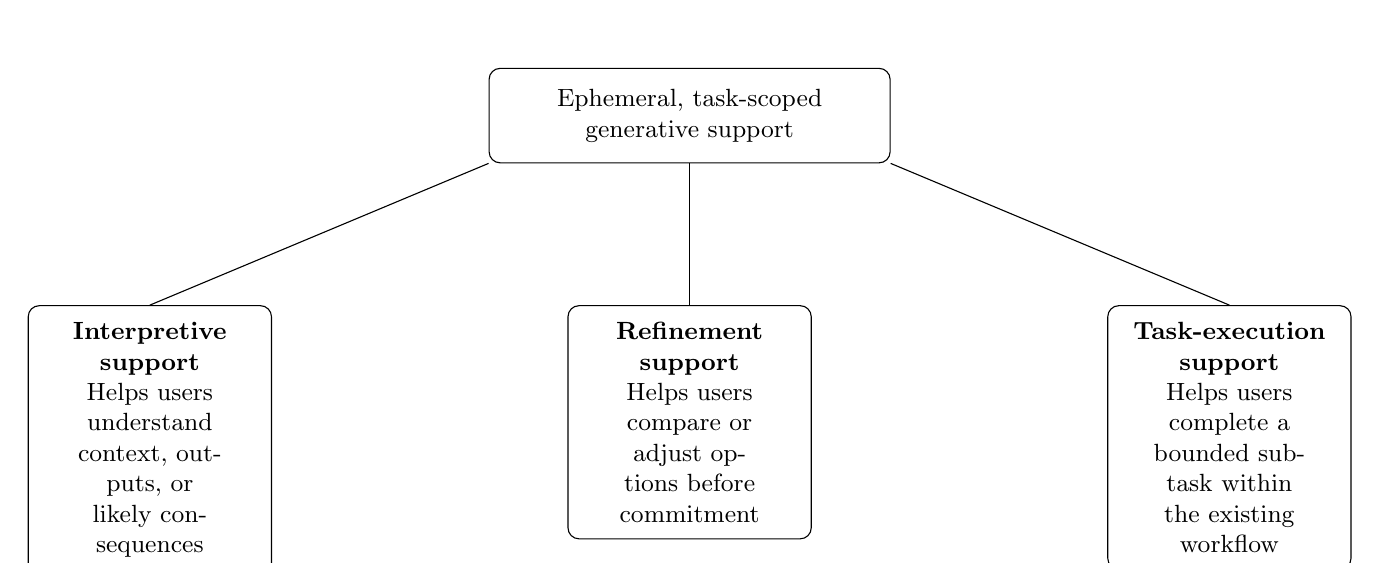
\begin{tikzpicture}[
        font=\small,
        box/.style={
            draw,
            rounded corners,
            align=center,
            text width=0.22\textwidth,
            minimum height=2.2cm,
            inner sep=6pt
        },
        topbox/.style={
            draw,
            rounded corners,
            align=center,
            minimum width=0.42\textwidth,
            minimum height=1.2cm,
            inner sep=6pt
        }
    ]

    \node[topbox] (root) {Ephemeral, task-scoped\\generative support};

    \node[box, below left=1.8cm and 2.75cm of root] (interpretive) {\textbf{Interpretive support}\\Helps users understand\\context, outputs, or\\likely consequences};
    \node[box, below=1.8cm of root] (refinement) {\textbf{Refinement support}\\Helps users compare or\\adjust options before\\commitment};
    \node[box, below right=1.8cm and 2.75cm of root] (execution) {\textbf{Task-execution support}\\Helps users complete a\\bounded subtask within\\the existing workflow};

    \draw[-] (root.south west) -- (interpretive.north);
    \draw[-] (root.south) -- (refinement.north);
    \draw[-] (root.south east) -- (execution.north);

    \end{tikzpicture}
    }
    \caption{Taxonomy of ephemeral, task-scoped generative support roles.}
    \label{fig:taxonomy}
\end{figure}

The second element is a lifecycle describing how an ephemeral component enters and leaves use. Alternative stage patterns can be found in the literature, ranging from the minimal logic of temporary appearance and disappearance to more scaffolded models in which users configure support before committing to an outcome. For this study, the most appropriate synthesis is a four-stage lifecycle of \emph{trigger}, \emph{instantiation}, \emph{interaction}, and \emph{dismissal}. A component is triggered when a clear user goal or contextual need is detected that is not adequately supported by the persistent interface alone. That trigger may be explicit, such as a user request for help, or inferred from local behavioural and contextual signals, but only when the resulting support remains low-risk, relevant, and easy to dismiss. The component is then instantiated as a temporary interface element embedded within the existing application rather than replacing the surrounding interface. During interaction, users inspect, steer, or complete the immediate subtask while remaining oriented within the primary workflow. Finally, the component is dismissed once the task is completed, abandoned, or no longer contextually relevant. This lifecycle was selected because it retains the conceptual clarity of ephemerality while remaining concrete enough to implement as a state-based interaction model in the artifact.

\begin{figure}[htbp]
    \centering
    \resizebox{0.95\textwidth}{!}{%
    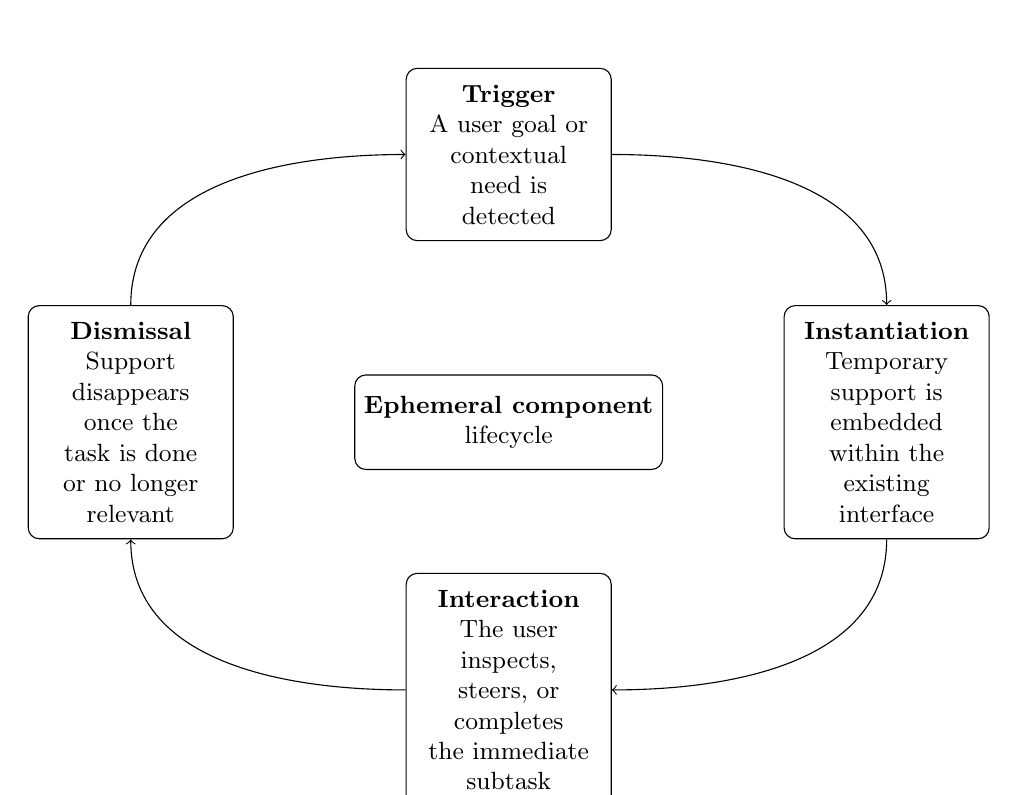
\begin{tikzpicture}[
        font=\small,
        stage/.style={
            draw,
            rounded corners,
            align=center,
            text width=0.18\textwidth,
            minimum height=2.0cm,
            inner sep=6pt
        }
    ]

    \node[draw, rounded corners, align=center, minimum width=3.4cm, minimum height=1.2cm] (core) at (0,0) {\textbf{Ephemeral component}\\lifecycle};

    \node[stage] (trigger) at (0,3.4) {\textbf{Trigger}\\A user goal or\\contextual need is\\detected};
    \node[stage] (instantiation) at (4.8,0) {\textbf{Instantiation}\\Temporary support is\\embedded within the\\existing interface};
    \node[stage] (interaction) at (0,-3.4) {\textbf{Interaction}\\The user inspects,\\steers, or completes\\the immediate subtask};
    \node[stage] (dismissal) at (-4.8,0) {\textbf{Dismissal}\\Support disappears\\once the task is done\\or no longer relevant};

    \draw[->] (trigger.east) to[out=0,in=90] (instantiation.north);
    \draw[->] (instantiation.south) to[out=-90,in=0] (interaction.east);
    \draw[->] (interaction.west) to[out=180,in=-90] (dismissal.south);
    \draw[->] (dismissal.north) to[out=90,in=180] (trigger.west);

    \end{tikzpicture}
    }
    \caption{Lifecycle of an ephemeral, task-scoped generative UI component: trigger, instantiation, interaction, and dismissal.}
    \label{fig:lifecycle}
\end{figure}

The third element is a set of design principles that constrain how ephemeral components should be introduced into an otherwise stable interface. Five principles guide the framework. \emph{Contextual relevance} means support should appear only when it serves a clear task-related purpose in the current situation. \emph{Bounded scope} means support should remain limited to the immediate subtask rather than taking over the larger workflow. \emph{Interface continuity} means the temporary component should preserve the surrounding page structure and the user's sense of place, rather than redirecting the interface toward an unrelated experience. \emph{User control} means users should be able to inspect, refine, confirm, or dismiss the support rather than being forced into a system decision. \emph{Graceful disappearance} means the component should recede cleanly once it is no longer needed. When support is inferred rather than explicitly invoked, these principles impose an additional safety constraint: inferred assistance may suggest or preload options, but it should not perform destructive or strongly consequential actions without explicit user confirmation. Together, these principles translate the theoretical idea of ephemerality into practical design criteria that can be applied consistently during artifact development and later assessed in the evaluation.

\subsection{Artifact Development}
The artifact developed in this project is a website used as a research instrument for evaluating the proposed framework in a controlled but realistic interaction setting. Rather than building a fully autonomous or fully generative application, the website is designed to preserve a recognisable baseline interface while allowing ephemeral, task-scoped components to be introduced at selected moments. This makes it possible to test whether the framework can augment an existing user experience without replacing the primary workflow altogether.

To operationalise the framework, the website will implement two interface conditions: an original condition representing the baseline experience and an ephemeral condition in which temporary, task-scoped components are introduced according to the taxonomy, lifecycle, and design principles defined above. The original condition will present the underlying tasks using a conventional persistent interface, whereas the ephemeral condition will surface temporary interface elements only when a user reaches a context in which additional guidance, refinement, or task support is needed. In this way, the comparison isolates the effect of ephemeral augmentation against the non-ephemeral alternative.

The website presents one scenario that represents a bounded productivity task within the application: a short presentation-refinement exercise foregrounding \emph{refinement support}. Participants receive a small slide deck and must improve its narrative order and clarify the problem slide before finalising it. The lifecycle of trigger, instantiation, interaction, and dismissal is implemented as the common interaction logic for both interface conditions. In the ephemeral condition, temporary support may propose grouping cues, comparisons, or lightweight controls that help the user adjust ordering and wording before commitment. Success is defined as producing a revised outline and problem statement that satisfy predefined task checks.

Although the ephemeral condition is allowed to be visually and structurally expressive, that expressiveness remains bounded by the framework. Temporary support may add task-relevant interface elements, annotate or highlight existing content, expose comparison views, or locally reconfigure a small region of the page. However, it does not replace the full application, arbitrarily reorganise the entire interface, or perform consequential actions without confirmation. In practice, the role category, lifecycle, task goals, and success criteria are fixed in advance, while local details such as wording, defaults, and the exact form of low-risk support may vary in response to immediate context. The ephemeral version is therefore not intended to be wholly different for every participant. Instead, it is constrained adaptation: users encounter the same scenario structures and the same framework rules, but the temporary support may be parameterised slightly differently within those limits. This preserves analytical robustness while still allowing the artifact to reflect the broader motivation of adaptive, goal-relevant ephemeral interfaces.

\subsection{Evaluation Design}

\subsubsection{Experimental Design}
The framework will be evaluated through a comparative within-subjects user study using the website artifact described above. Each participant will complete two trials in total: the same slide-refinement scenario once under the original baseline condition and once under the ephemeral condition, in an order randomised per participant. A within-subjects design is appropriate because it allows each participant to act as their own control, thereby reducing the influence of individual differences in digital literacy, task strategy, or prior familiarity with similar interfaces. Trial order will be randomised within the website so that participants encounter both conditions without a systematic sequence bias.

\subsubsection{Participants}
Participants will be recruited as regular users of web-based applications who can complete common digital tasks in a desktop browser environment. Recruitment will follow a convenience sampling approach appropriate to the scope of the capstone project. Inclusion criteria will focus on participants who are able to use standard web interfaces independently, while any exclusion criteria will be limited to factors that would prevent valid completion of the study tasks. The final sample size will depend on recruitment feasibility, but the study is designed to support repeated-measures comparisons between the two interface conditions.

\subsubsection{Materials and Procedure}
The primary study material is the experimental website, which implements both the original and ephemeral interface conditions. Participants will complete one bounded scenario twice: a presentation-style refinement task in which they adjust slide order and clarifying text. The task structure, goals, and success criteria remain constant for all users so that the study remains comparable across sessions. Within that shared structure, the ephemeral condition may vary in how temporary support is presented so that the assistance can respond to local context while remaining constrained by predefined design rules derived from the framework. In other words, the study does not test unlimited personalisation or unrestricted interface takeover. It tests bounded interface adaptation in which temporary support may add, highlight, compare, or locally rearrange elements while preserving interface continuity and user control.

The procedure will be fully website-based. After opening the study website, participants will read the study information, provide consent, and complete a short background questionnaire about their comfort with websites and familiarity with AI-assisted tools. The website will then present two task trials in a randomised order, representing the same scenario under the original baseline and ephemeral conditions. Before each trial, participants will receive a short task prompt that labels the interface version for fair debriefing. During each trial, the website will automatically log behavioural data. After each trial, participants will complete brief ratings on intrusiveness, perceived control, and helpfulness. After both trials are complete, participants will answer a final comparative questionnaire about overall preference between the two conditions, with an explicit reminder of which version corresponded to assistance for that participant. This fully instrumented procedure keeps the study structure consistent while allowing all behavioural and self-reported data to be collected in the same environment.

\subsubsection{Measures}
The evaluation combines behavioural and self-reported measures in order to capture both task performance and perceived experience. Behavioural measures are derived from interaction logs recorded by the website, while subjective measures are collected through short post-trial and post-study questionnaires. The core claim being tested is not simply that ephemeral interfaces are preferred, but that they can improve task support without introducing additional disruption. To assess that claim, the study will measure efficiency through task completion time, effectiveness through task completion rate, friction through interaction count, and user experience through ratings of intrusiveness, perceived control, helpfulness, and overall preference. In addition, ephemeral-only interaction logs will record whether temporary support was opened, used, refined, dismissed, or ignored, allowing the study to interpret how participants actually engaged with the generated assistance.

\begin{table}[htbp]
    \centering
    \caption{Dependent measures and collection methods.}
    \label{tab:measures}
    \begin{tabular}{@{}llll@{}}
        \toprule
        Measure & Type & Collection & Analysis \\
        \midrule
        Task completion rate & Binary & Event logging & Paired categorical comparison \\
        Task completion time & Continuous & Timestamps & Paired comparison \\
        Interaction count & Discrete & Event logging & Paired comparison \\
        Intrusiveness & Ordinal (1--7) & Post-trial Likert item & Paired comparison \\
        Perceived control & Ordinal (1--7) & Post-trial Likert item & Paired comparison \\
        Helpfulness & Ordinal (1--7) & Post-trial Likert item & Paired comparison \\
        Preference & Nominal & Final forced choice & Comparative choice analysis \\
        \bottomrule
    \end{tabular}
\end{table}

\subsubsection{Data Collection}
Data collection will combine instrumented event logging with questionnaire responses. For each trial, the website will record task start and end times, completion outcomes, interaction counts, and the active interface condition. In the ephemeral condition, additional logs will capture component trigger events, support openings, dismissals, confirmations, and refinement actions. Post-trial survey items will capture perceived intrusiveness, perceived control, and helpfulness, while the final questionnaire will capture overall preference between conditions. To link behavioural and survey data, each session will be associated with a participant identifier that is stored consistently across the website logs and questionnaire responses.

\subsubsection{Analysis Plan}
The primary analysis will compare the original and ephemeral conditions on each dependent measure using repeated-measures statistical tests appropriate to the data type and distribution. Task completion rate will be analysed as a paired categorical outcome, while time, interaction count, and subjective ratings will be analysed using paired comparisons, with non-parametric alternatives considered if distributional assumptions are not met. Preference will be analysed as a comparative choice measure. Ephemeral-only interaction logs will be analysed descriptively to show whether support was typically accepted, refined, or dismissed, which helps interpret whether a null or positive effect reflects the quality of the support itself or low uptake. The analysis will therefore focus on whether the ephemeral condition yields improvements in efficiency, effectiveness, or perceived helpfulness without increasing intrusiveness or reducing perceived control. Because the ephemeral experience may vary within bounded framework rules, the analysis treats that variation as part of the intended adaptive behaviour of the artifact rather than as an uncontrolled change to the task itself.
\pagestyle{fancy}
\section{Implementation}\label{sec:implementation}

The previous section defined the conceptual framework, the artifact's purpose as a research instrument, and the evaluation design that structures the comparative study. This section describes how those ideas were translated into a working system. The goal is not to document every engineering decision, but to make the technical design legible enough that the reader can assess whether the artifact faithfully operationalises the framework and whether the instrumentation is sufficient to support the evaluation.

\subsection{Architecture Overview}

The artifact is built as a full-stack web application using the Next.js App Router with TypeScript. The server layer exposes a set of API routes that handle participant management, trial orchestration, event logging, questionnaire storage, and ephemeral support generation. Persistent data is stored in a PostgreSQL database accessed through Drizzle~ORM, which provides type-safe queries and a migration-based schema workflow. The ephemeral support system relies on Google Gemini, accessed through the Vercel AI~SDK, to produce structured interface specifications from the current task state. The front end uses Tailwind~CSS and a component library based on Radix~UI primitives for consistent, accessible interface elements across both experimental conditions.

These choices reflect the requirements of a research instrument rather than a production application. Next.js was selected because its App Router collocates server-side logic and client rendering in the same project, which simplifies the instrumentation of both request handling and user interaction. TypeScript and Zod provide compile-time and runtime type safety across the generation pipeline, which is critical when validating AI-generated output against a constrained specification. PostgreSQL and Drizzle offer relational integrity and migration tooling appropriate for structured experimental data. The Vercel AI~SDK abstracts provider-specific details while supporting structured output modes, which allows the generation step to request JSON that conforms to a predefined schema rather than parsing free-form text.

\begin{figure}[htbp]
    \centering
    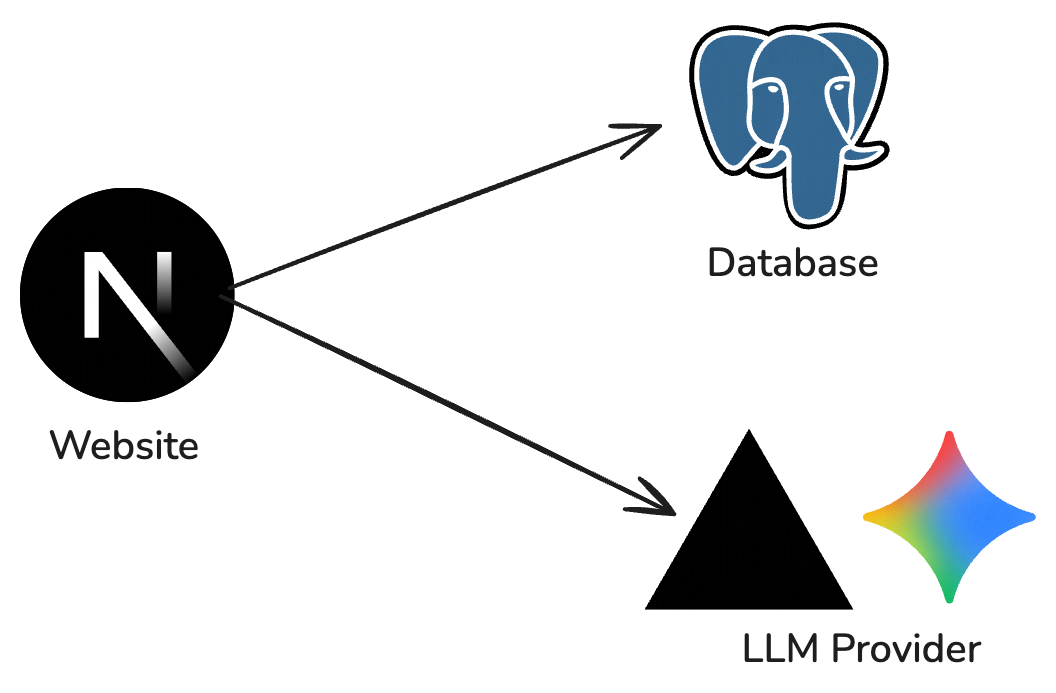
\includegraphics[width=0.95\textwidth]{graphics/architecture.png}
    \caption{High-level system architecture of the experimental artifact.}
    \label{fig:architecture}
\end{figure}

\subsection{Participant Flow and Session Management}

The study procedure described in the methodology is implemented as a linear state machine that determines which page the participant should see at any point during the session. When a participant first opens the website, they are presented with the study information and consent form. Providing consent creates a participant record in the database and sets an HTTP-only session cookie that associates all subsequent requests with that record. No traditional authentication is required because the study collects no directly identifying personal data; the cookie serves only to link a browser session to its corresponding participant row.

After consenting, the participant completes a short background questionnaire covering age range, occupation, familiarity with web applications, and familiarity with AI-assisted tools. Submitting the background questionnaire acknowledges the study instructions and triggers the creation of the first trial row. From this point forward, a server-side state resolution function inspects the participant's record, their trial rows, and their questionnaire responses to determine the current study step. The possible steps form a fixed sequence: \emph{background}, \emph{study} (an active trial), \emph{post-trial questionnaire}, \emph{final questionnaire}, and \emph{complete}. The client-side routing function maps each step to the corresponding page, so that refreshing the browser or navigating away always returns the participant to the correct point in the procedure.

Trial rows are created incrementally rather than all at once. The first trial is created when the participant acknowledges the instructions. Each subsequent trial is created only after the previous trial has been completed and its post-trial questionnaire has been submitted. This ensures that the participant cannot skip ahead or access later trials before finishing earlier ones.

Counterbalancing is implemented at the participant level. When a participant record is created, a boolean flag is randomly set to determine whether the baseline condition corresponds to Version~A or Version~B. The trial plan then assigns conditions to version labels using this flag, so that one participant may encounter the baseline first while another encounters the ephemeral condition first, both under the neutral label ``Version~A.'' The content variant for each condition is further diversified by hashing the participant identifier together with the scenario identifier, ensuring that the specific slide deck a participant sees in the baseline condition differs from the one they see in the ephemeral condition.

\subsection{Data Model}

The database schema consists of five tables designed to capture the behavioural and self-reported data required by the evaluation measures defined in the methodology. Figure~\ref{fig:data-model-erd} shows the entity--relationship structure: each participant may complete several trials; each trial may emit many logged events and many stored ephemeral support generations; questionnaire responses belong to a participant, and may optionally reference a trial (post-trial items) or omit a trial key (final questionnaire). Table~\ref{tab:schema} summarises what each table contributes to the evaluation. The \texttt{trial\_events} table also stores \texttt{participant\_id} for efficient querying, in addition to \texttt{trial\_id}; the diagram omits that redundant edge for clarity.

\begin{figure}[htbp]
    \centering
    \resizebox{0.95\textwidth}{!}{%
    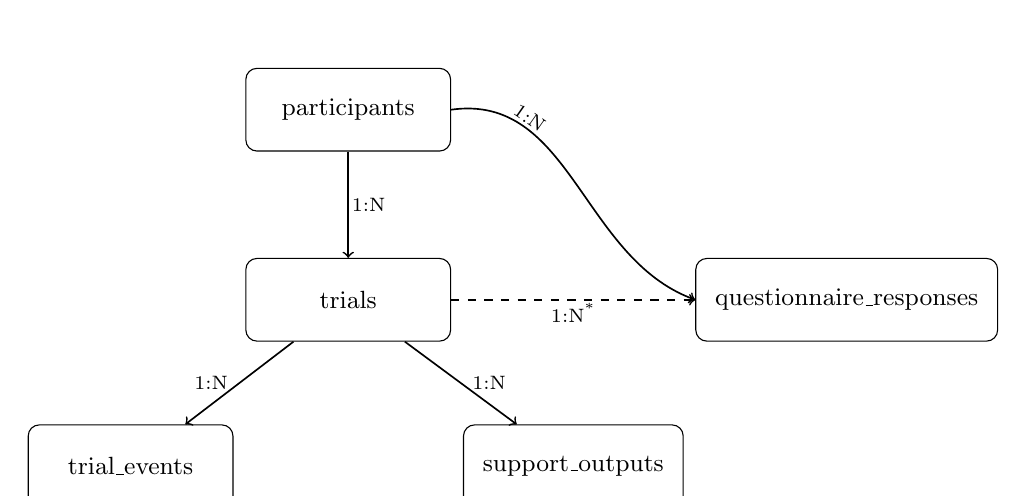
\begin{tikzpicture}[
        font=\small,
        ent/.style={
            draw,
            rounded corners,
            align=center,
            inner sep=7pt,
            minimum width=2.6cm,
            minimum height=1.05cm
        },
        card/.style={font=\scriptsize, inner sep=1pt}
    ]
    \node[ent] (P) {participants};
    \node[ent, below=1.35cm of P] (T) {trials};
    \node[ent, below left=1.05cm and 0.15cm of T] (E) {trial\_events};
    \node[ent, below right=1.05cm and 0.15cm of T] (S) {support\_outputs};
    \node[ent, right=3.1cm of T] (Q) {questionnaire\_responses};

    \draw[->, semithick] (P) -- node[card, right] {1:N} (T);
    \draw[->, semithick] (T) -- node[card, left, xshift=-1mm] {1:N} (E);
    \draw[->, semithick] (T) -- node[card, right, xshift=1mm] {1:N} (S);
    \draw[->, semithick] (P.east) to[out=8, in=160] node[card, above, sloped, near start] {1:N} (Q.west);
    \draw[->, semithick, dashed] (T.east) -- node[card, below, midway] {1:N\textsuperscript{*}} (Q.west);
    \end{tikzpicture}%
    }
    \caption{Entity--relationship diagram of the study database. Directed edges are labelled with cardinalities: one participant to many trials; one trial to many events and many support records; one participant to many questionnaire rows. The dashed edge indicates an optional foreign key: \texttt{trial\_id} is \texttt{NULL} for final-questionnaire rows.}
    \label{fig:data-model-erd}
\end{figure}

\begin{table}[htbp]
    \centering
    \small
    \caption{Summary of each table's role relative to the evaluation measures. Full column definitions follow the Drizzle schema in the artifact.}
    \label{tab:schema}
    \begin{tabular}{@{}p{0.28\textwidth}p{0.62\textwidth}@{}}
        \toprule
        Table & Role in the study \\
        \midrule
        \texttt{participants} & Consent and background questionnaire; counterbalancing flag (\texttt{baseline\_is\_version\_a}); links all rows for a session. \\
        \texttt{trials} & One row per task trial: condition, scenario, timing, correctness, submitted answer, interaction count---supports performance and efficiency measures. \\
        \texttt{trial\_events} & Typed events with JSON payloads---supports interaction counts and ephemeral engagement (e.g.\ support shown, dismissed). \\
        \texttt{questionnaire\_responses} & Post-trial Likert items and final preference; \texttt{trial\_id} set for post-trial rows, null for final rows---supports subjective measures. \\
        \texttt{support\_outputs} & Ephemeral condition only: model input state and output spec per generation---supports analysis of support quality and fallback. \\
        \bottomrule
    \end{tabular}
\end{table}

Foreign key constraints with cascading deletion ensure referential integrity: deleting a participant removes all associated trials, events, questionnaire responses, and support outputs. Indexes on participant identifiers, trial identifiers, and event types support efficient querying during data export and analysis.

\subsection{Task Scenario Implementation}

The study evaluates one scenario, the slide-reordering task described in the methodology, under two experimental conditions. The implementation uses a scenario registry that defines each scenario's metadata, including its taxonomy category, correct answer, allowed ephemeral targets, task prompts, and a function that builds the initial task state. This registry-based design means that adding a new scenario requires only a new registry entry rather than changes to the study flow or state machine.

The slide-reordering scenario presents participants with a short deck of four slides whose order has been intentionally scrambled. The main canvas area displays a read-only preview of the currently selected slide, while the actual task interaction occurs through a horizontal strip of draggable thumbnail cards. Drag-and-drop is implemented using the \texttt{@dnd-kit} library, which provides accessible keyboard and pointer-based reordering with sortable constraints. Participants reorder the strip and submit when they believe the sequence is correct.

Correctness is evaluated by comparing the submitted slide order against a predefined canonical order. Each scenario variant defines its own canonical sequence: variant~A follows a corporate readout structure (title, problem, metrics, ask), while variant~B follows a committee funding structure (meeting frame, policy, proof, ballot items). The variant assignment uses a deterministic hash of the participant identifier and scenario identifier to assign variant~A or variant~B to the baseline condition, with the opposite variant assigned to the ephemeral condition. This ensures that each participant encounters two different slide decks across the two trials, preventing familiarity effects from the task content while keeping the task structure identical.

Both conditions share the same task component, the same interaction mechanics, and the same submission logic. The only difference is whether the ephemeral support layer is active, which is controlled by the condition field on the trial row. This design isolates the effect of ephemeral augmentation from other variables.

\subsection{Ephemeral Support System}

The ephemeral support system is the core technical contribution of the artifact. It translates the framework's concepts of taxonomy, lifecycle, and design principles into a constrained generative pipeline that produces temporary interface overlays without replacing the host application. This subsection describes the three layers of the system: the specification model that defines what can be generated, the pipeline that produces and validates specifications, and the rendering layer that displays them.

\subsubsection{Component Specification Model}

Ephemeral support is represented as a typed tree structure called an \texttt{EphemeralSpec}. Each specification contains a version number, a root node, and metadata indicating whether the overlay is dismissible. Nodes are recursive: each node has a type, a property bag validated against a per-type schema, and optional children. The tree is constrained to a maximum depth of four levels and a maximum of six children per node.

The component catalog defines seventeen component types, organised into five functional categories. Table~\ref{tab:component-catalog} lists the types and their roles. Visual cue components draw attention to specific interface elements without adding content. Anchored annotation components attach textual or rich content near a target element. Relational components connect or compare two or more targets to support reasoning across elements. Layout containers position children within the viewport or relative to a target. Rich content components render sanitised HTML and inline SVG for more expressive explanations such as flow diagrams or annotated illustrations.

\begin{table}[htbp]
    \centering
    \small
    \caption{Ephemeral component catalog (version~3). Each type is validated against a per-component Zod schema that enforces field types, string lengths, and structural constraints.}
    \label{tab:component-catalog}
    \begin{tabular}{@{}p{0.22\textwidth}p{0.26\textwidth}p{0.44\textwidth}@{}}
        \toprule
        Category & Component type & Role \\
        \midrule
        Visual cues & \texttt{HighlightRing} & Amber ring around a target element \\
        & \texttt{PulseRing} & Animated ring with configurable duration \\
        & \texttt{ArrowCue} & Arrow pointing at a target \\
        & \texttt{FocusMask} & Dims everything except the target \\
        \midrule
        Anchored annotations & \texttt{AnchoredTooltip} & Plain-text tooltip near a target \\
        & \texttt{HintStack} & Ordered list of short hints near a target \\
        & \texttt{InspectPanel} & Expandable panel with summary and optional detail lines \\
        & \texttt{ConsequenceNote} & Single italic consequence line near a target \\
        & \texttt{SideNote} & Margin annotation beside a target \\
        \midrule
        Relational & \texttt{ConnectorLine} & Dashed line between two targets \\
        & \texttt{ComparisonStrip} & Short contrast text positioned under two targets \\
        & \texttt{StepRail} & Numbered callouts across two to six targets \\
        \midrule
        Layout containers & \texttt{Stack} & Vertical sequence container \\
        & \texttt{ViewportPanel} & Absolutely positioned panel in viewport percentages \\
        & \texttt{TargetOffsetPanel} & Panel positioned relative to a target with pixel offsets \\
        \midrule
        Rich content & \texttt{FlowHtml} & Sanitised HTML block (only inside \texttt{ViewportPanel}) \\
        & \texttt{AnchoredHtml} & Sanitised HTML anchored near a target \\
        \bottomrule
    \end{tabular}
\end{table}

Each component type is associated with a Zod schema that validates its properties at runtime. These schemas enforce constraints such as maximum string lengths, numeric ranges, and required fields. For example, an \texttt{InspectPanel} requires a target identifier, a title of at most 120~characters, a summary of at most 280~characters, and optionally up to four detail lines of at most 200~characters each. These limits prevent the model from generating excessively long or unbounded output while leaving enough room for contextually relevant content.

The catalog is versioned so that changes to the available component types or their constraints can be tracked across study sessions. The current study uses catalog version~3.

\subsubsection{Generation and Validation Pipeline}\label{sec:pipeline}

When ephemeral support is requested during a trial, the system executes a multi-stage pipeline that generates a specification, validates it against the catalog and scenario constraints, and either accepts it or falls back to a deterministic alternative. Figure~\ref{fig:ephemeral-pipeline-impl} illustrates this pipeline.

The generation step constructs two prompts. The system prompt describes the specification schema, lists all available component types with their property schemas, states the allowed target identifiers for the current scenario, provides taxonomy-specific guidance (such as which components are most appropriate for refinement support), and enumerates the design rules that constrain output structure. The user prompt includes the current task state, including slide order, deck metadata, and review goals, together with an optional participant interaction snapshot that reflects the participant's progress at the moment support was requested. This snapshot allows the model to tailor its output to what the participant has already done rather than generating generic first-visit guidance.

The system sends these prompts to Google Gemini using the Vercel AI~SDK's structured output mode, which constrains the model to produce JSON conforming to a provided Zod schema. The schema used for model output is a simplified subset of the full specification schema, designed to avoid compatibility issues with the provider's structured output implementation while remaining strict enough to prevent most structural errors at generation time.

The model's output then passes through a series of server-side validation stages:

\begin{enumerate}
    \item \textbf{Envelope parsing.} The top-level structure is checked for a valid version number, root node, and metadata.
    \item \textbf{Node tree parsing.} The root and its descendants are recursively validated for correct node shape, child count limits, and maximum depth.
    \item \textbf{Per-component property validation.} Each node's properties are validated against its type-specific Zod schema, enforcing field types, string lengths, and numeric ranges.
    \item \textbf{Target allowlisting.} Every target identifier referenced in the specification is checked against the scenario's predefined list of allowed targets. Any reference to an interface element not declared in the scenario registry causes the specification to be rejected.
    \item \textbf{Structural container rules.} Layout containers are checked to ensure they contain at least one child. This applies to \texttt{Stack}, \texttt{ViewportPanel}, and \texttt{TargetOffsetPanel}.
    \item \textbf{Ancestry constraints.} \texttt{FlowHtml} nodes are permitted only within a \texttt{ViewportPanel} subtree, preventing free-floating rich HTML from appearing anywhere in the interface.
    \item \textbf{HTML sanitisation.} Any HTML content in \texttt{FlowHtml}, \texttt{AnchoredHtml}, or \texttt{SideNote} nodes is passed through a server-side sanitisation step using DOMPurify with a strict allowlist of tags and attributes. This prevents injection of scripts, event handlers, or disallowed elements while permitting semantic HTML and inline SVG for diagrams.
\end{enumerate}

If any stage rejects the output, the system falls back to a deterministic, hardcoded specification for the current scenario. Fallback specifications are defined per scenario and per variant, ensuring that every participant in the ephemeral condition receives some form of support regardless of model behaviour. The fallback specifications use the same component types and target identifiers as model-generated output, so they appear visually consistent with the rest of the ephemeral experience.

Whether the specification was model-generated or a fallback, the full input state, model name, and output are persisted to the \texttt{support\_outputs} table. This logging enables post-study analysis of generation quality, fallback frequency, and the relationship between input context and output content.

To verify this implementation end-to-end outside the aggregate study analysis, the pipeline was also tested locally against the real \texttt{/api/support} route on 2026-04-04. Three consecutive hesitation-triggered requests for the \texttt{slides-outline-refine} scenario completed successfully and were persisted as \texttt{support\_outputs} rows 101--103, all with \texttt{usedFallback = false} and \texttt{modelName = gemini-2.0-flash}. The richest of these records (row 103) produced a \texttt{Stack}-rooted specification containing \texttt{StepRail}, \texttt{InspectPanel}, \texttt{ConnectorLine}, and \texttt{AnchoredTooltip} nodes, demonstrating that a non-trivial multi-component overlay could be generated, validated, saved to PostgreSQL, and rendered without falling back. A condensed excerpt of this local trace is included in Appendix~\ref{app:local-generation-trace}.

\begin{figure}[htbp]
    \centering
    \resizebox{0.98\textwidth}{!}{%
    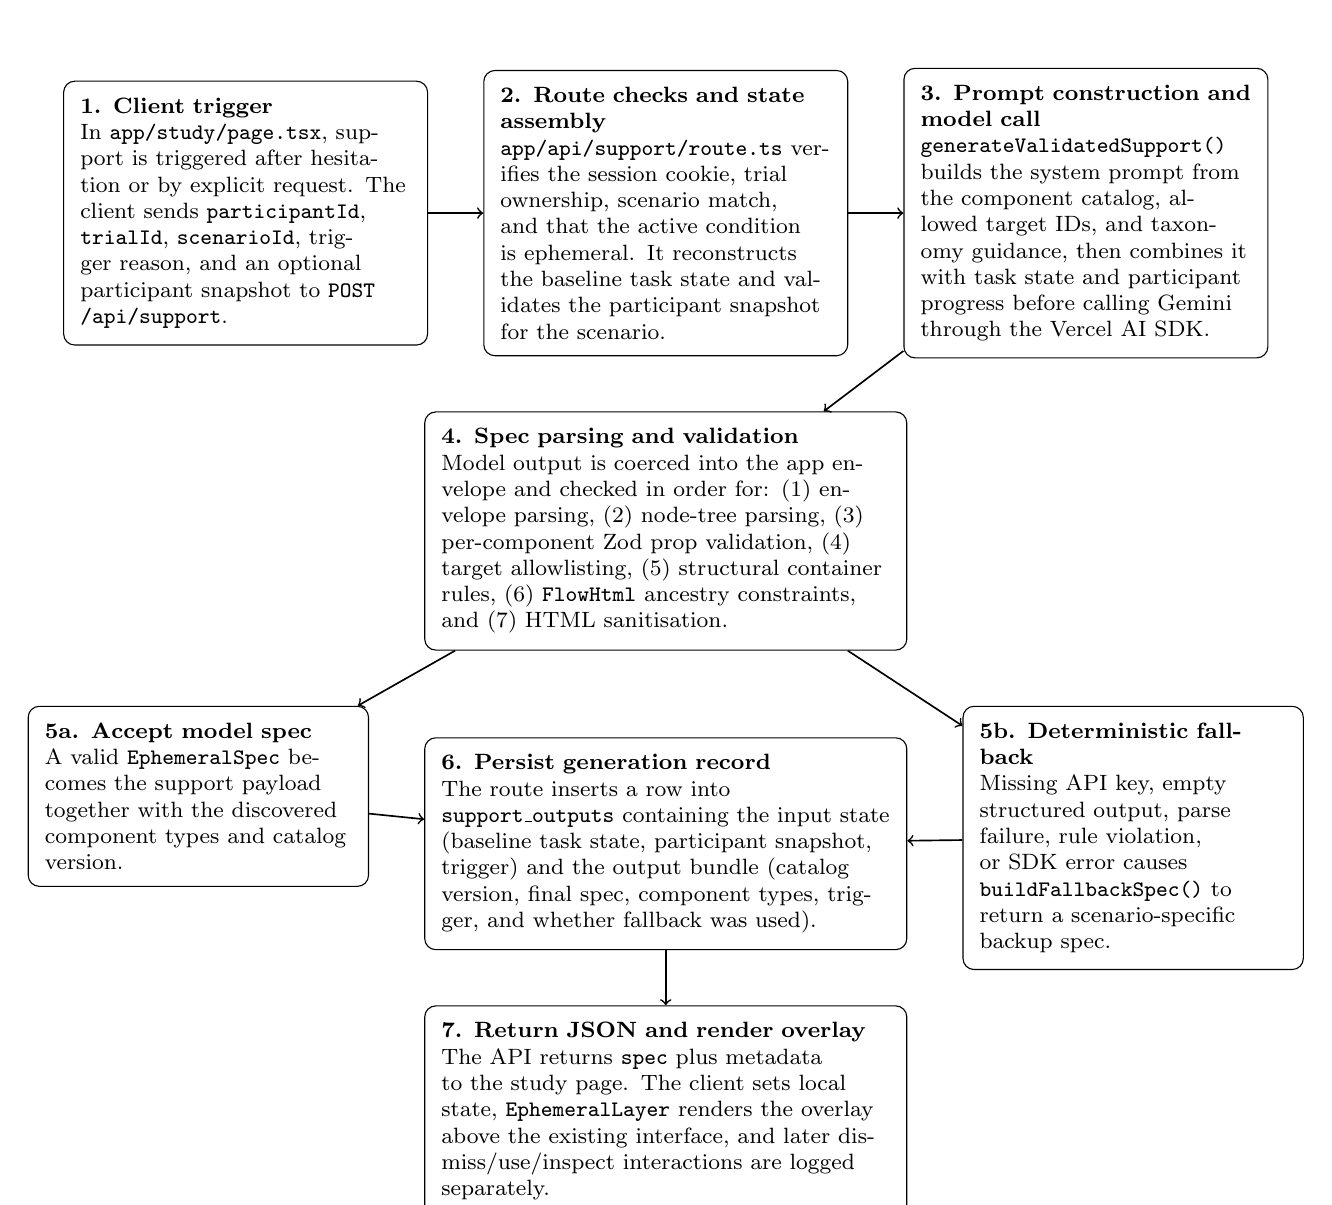
\begin{tikzpicture}[
        font=\footnotesize,
        node distance=7mm and 7mm,
        box/.style={
            draw,
            rounded corners,
            align=left,
            inner sep=6pt,
            text width=4.2cm
        },
        wide/.style={
            draw,
            rounded corners,
            align=left,
            inner sep=6pt,
            text width=5.7cm
        },
        small/.style={
            draw,
            rounded corners,
            align=left,
            inner sep=6pt,
            text width=3.9cm
        }
    ]
    \node[box] (trigger) {\textbf{1. Client trigger}\\
    In \texttt{app/study/page.tsx}, support is triggered after hesitation or by explicit request. The client sends \texttt{participantId}, \texttt{trialId}, \texttt{scenarioId}, trigger reason, and an optional participant snapshot to \texttt{POST /api/support}.};

    \node[box, right=of trigger] (route) {\textbf{2. Route checks and state assembly}\\
    \texttt{app/api/support/route.ts} verifies the session cookie, trial ownership, scenario match, and that the active condition is ephemeral. It reconstructs the baseline task state and validates the participant snapshot for the scenario.};

    \node[box, right=of route] (prompt) {\textbf{3. Prompt construction and model call}\\
    \texttt{generateValidatedSupport()} builds the system prompt from the component catalog, allowed target IDs, and taxonomy guidance, then combines it with task state and participant progress before calling Gemini through the Vercel AI SDK.};

    \node[wide, below=of route] (validate) {\textbf{4. Spec parsing and validation}\\
    Model output is coerced into the app envelope and checked in order for: (1) envelope parsing, (2) node-tree parsing, (3) per-component Zod prop validation, (4) target allowlisting, (5) structural container rules, (6) \texttt{FlowHtml} ancestry constraints, and (7) HTML sanitisation.};

    \node[small, below left=of validate] (accept) {\textbf{5a. Accept model spec}\\
    A valid \texttt{EphemeralSpec} becomes the support payload together with the discovered component types and catalog version.};

    \node[small, below right=of validate] (fallback) {\textbf{5b. Deterministic fallback}\\
    Missing API key, empty structured output, parse failure, rule violation, or SDK error causes \texttt{buildFallbackSpec()} to return a scenario-specific backup spec.};

    \node[wide, below=11mm of validate] (persist) {\textbf{6. Persist generation record}\\
    The route inserts a row into \texttt{support\_outputs} containing the input state (baseline task state, participant snapshot, trigger) and the output bundle (catalog version, final spec, component types, trigger, and whether fallback was used).};

    \node[wide, below=of persist] (render) {\textbf{7. Return JSON and render overlay}\\
    The API returns \texttt{spec} plus metadata to the study page. The client sets local state, \texttt{EphemeralLayer} renders the overlay above the existing interface, and later dismiss/use/inspect interactions are logged separately.};

    \draw[->, semithick] (trigger) -- (route);
    \draw[->, semithick] (route) -- (prompt);
    \draw[->, semithick] (prompt) -- (validate);
    \draw[->, semithick] (validate) -- (accept);
    \draw[->, semithick] (validate) -- (fallback);
    \draw[->, semithick] (accept) -- (persist);
    \draw[->, semithick] (fallback) -- (persist);
    \draw[->, semithick] (persist) -- (render);
    \end{tikzpicture}%
    }
    \caption{Ephemeral support generation and validation pipeline. Model output passes through seven validation stages before rendering; invalid output triggers a deterministic fallback. Both paths are logged for later analysis.}
    \label{fig:ephemeral-pipeline-impl}
\end{figure}

\subsubsection{Rendering Layer}

Accepted specifications are rendered as a temporary overlay above the existing application interface using a React portal. The overlay component receives the validated specification tree and recursively dispatches each node to its corresponding catalog component based on the node's type. This dispatch model means that the renderer does not need to know about the content of any particular specification; it only needs to map types to components and pass through validated properties.

Components that reference target elements, such as \texttt{HighlightRing}, \texttt{AnchoredTooltip}, or \texttt{ConnectorLine}, resolve their targets by looking up DOM elements by identifier. A custom hook observes the target element's bounding rectangle and updates the overlay position when the layout changes, for example when the browser is resized or when other elements shift. A viewport clamping utility ensures that anchored components remain visible even when their target is near the edge of the screen.

The overlay respects the lifecycle stage of dismissal defined in the framework. When the specification's metadata marks the overlay as dismissible, a close control is rendered that allows the participant to remove the support at any time. Dismissal fires a logged event so that the analysis can distinguish between support that was actively used and support that was dismissed without engagement. The overlay does not persist across page navigations or trial boundaries, which enforces the ephemerality principle at the session level.

\subsection{Instrumentation and Logging}

The evaluation design in the methodology specifies several behavioural and self-reported measures. The artifact implements a corresponding instrumentation layer that captures the data needed for each measure.

Client-side interaction events are sent to a logging API endpoint that inserts rows into the \texttt{trial\_events} table. Each event includes a type label and a JSON payload with contextual details. A predefined set of event types is recognised as countable interactions, and the trial's running interaction count is incremented automatically when one of these events is recorded. Table~\ref{tab:event-types} lists the event types and their relationship to the evaluation measures.

\begin{table}[htbp]
    \centering
    \small
    \caption{Logged event types and their relationship to evaluation measures. Events marked with an asterisk (*) increment the trial's interaction count.}
    \label{tab:event-types}
    \begin{tabular}{@{}p{0.33\textwidth}p{0.41\textwidth}p{0.18\textwidth}@{}}
        \toprule
        Event type & When recorded & Evaluation measure \\
        \midrule
        \texttt{trial\_viewed}* & Participant opens a trial & Interaction count \\
        \texttt{slide\_reordered}* & A slide is dragged to a new position & Interaction count \\
        \texttt{answer\_selected}* & An answer is first chosen & Interaction count \\
        \texttt{answer\_changed}* & An answer is revised & Interaction count \\
        \midrule
        \texttt{support\_requested}* & Participant explicitly requests support & Support engagement \\
        \texttt{support\_triggered}* & Support is triggered automatically & Support engagement \\
        \texttt{support\_shown}* & Support overlay becomes visible & Support engagement \\
        \texttt{support\_dismissed}* & Participant closes the overlay & Support engagement \\
        \texttt{support\_used}* & Participant acts on the support & Support engagement \\
        \texttt{support\_ignored}* & Support is present but not interacted with & Support engagement \\
        \texttt{support\_inspect\_expanded}* & Participant expands an \texttt{InspectPanel} detail section & Support engagement \\
        \bottomrule
    \end{tabular}
\end{table}

For the ephemeral condition, additional data is captured beyond interaction events. Each call to the support generation endpoint persists the full input state (task state and participant snapshot), the model name, and the complete output specification to the \texttt{support\_outputs} table. This allows the analysis to examine not only whether support was shown and used, but also what the system produced and why, including whether a fallback was triggered.

Questionnaire responses are stored as individual question--response pairs rather than as monolithic form submissions. Post-trial ratings for intrusiveness, perceived control, and helpfulness are linked to the specific trial they follow, while final comparative questions are linked only to the participant. This structure supports direct joins between behavioural data and subjective ratings at the trial level.

A data export endpoint produces a structured bundle of all study data, protected by a server-side secret. The export includes participant records, trial summaries with performance metrics, event logs, questionnaire responses, and support generation outputs, providing the complete dataset needed for the analysis plan described in the methodology.

\pagestyle{fancy}
\section{Results}
% AUTO-GENERATED by analysis/generate-results-tex.ts — do not edit by hand.
% Regenerate: cd analysis && bun run gen-tex

\providecommand{\GenNTotal}{0}
\providecommand{\GenNValid}{19}
\providecommand{\GenDemoAge}{19 (5); 20 (1); 21 (3); 22 (6); 23 (3); 24 (1)}
\providecommand{\GenDemoWebMdn}{6.0}
\providecommand{\GenDemoWebIqr}{6.0--7.0}
\providecommand{\GenDemoAiMdn}{6.0}
\providecommand{\GenDemoAiIqr}{5.0--7.0}
\providecommand{\GenCounterBaselineFirstN}{11}
\providecommand{\GenCounterBaselineFirstPct}{58}
\providecommand{\GenCounterEphemeralFirstN}{8}
\providecommand{\GenCounterEphemeralFirstPct}{42}
\providecommand{\GenCompNBaseline}{11}
\providecommand{\GenCompNEphemeral}{13}
\providecommand{\GenCompPctBaseline}{57.9}
\providecommand{\GenCompPctEphemeral}{68.4}
\providecommand{\GenCompMcNemarP}{0.500}
\providecommand{\GenTimeBaselineMdn}{35.7}
\providecommand{\GenTimeBaselineIqr}{16.4--73.4}
\providecommand{\GenTimeEphemeralMdn}{56.9}
\providecommand{\GenTimeEphemeralIqr}{23.0--85.1}
\providecommand{\GenTimeWilcoxonResult}{did not yield a statistically significant difference}
\providecommand{\GenTimeW}{80}
\providecommand{\GenTimeP}{0.568}
\providecommand{\GenTimeR}{0.158}
\providecommand{\GenIntBaselineMdn}{3.0}
\providecommand{\GenIntBaselineIqr}{1.0--4.0}
\providecommand{\GenIntEphemeralMdn}{11.0}
\providecommand{\GenIntEphemeralIqr}{5.0--13.0}
\providecommand{\GenIntWilcoxonResult}{yielded a statistically significant difference}
\providecommand{\GenIntW}{0}
\providecommand{\GenIntP}{\textless 0.001}
\providecommand{\GenIntR}{1.000}
\providecommand{\GenLikertHelpfulnessBaselineMdn}{5.0}
\providecommand{\GenLikertHelpfulnessBaselineIqr}{3.0--6.0}
\providecommand{\GenLikertHelpfulnessEphemeralMdn}{6.0}
\providecommand{\GenLikertHelpfulnessEphemeralIqr}{5.0--6.0}
\providecommand{\GenLikertHelpfulnessP}{0.048}
\providecommand{\GenLikertIntrusivenessBaselineMdn}{3.0}
\providecommand{\GenLikertIntrusivenessBaselineIqr}{2.0--5.0}
\providecommand{\GenLikertIntrusivenessEphemeralMdn}{5.0}
\providecommand{\GenLikertIntrusivenessEphemeralIqr}{4.0--6.0}
\providecommand{\GenLikertIntrusivenessP}{0.021}
\providecommand{\GenLikertControlBaselineMdn}{6.0}
\providecommand{\GenLikertControlBaselineIqr}{4.5--7.0}
\providecommand{\GenLikertControlEphemeralMdn}{6.0}
\providecommand{\GenLikertControlEphemeralIqr}{4.5--6.0}
\providecommand{\GenLikertControlP}{0.635}
\providecommand{\GenPrefOverallB}{4}
\providecommand{\GenPrefOverallE}{9}
\providecommand{\GenPrefOverallN}{6}
\providecommand{\GenPrefHelpB}{6}
\providecommand{\GenPrefHelpE}{10}
\providecommand{\GenPrefHelpN}{3}
\providecommand{\GenPrefIntrB}{1}
\providecommand{\GenPrefIntrE}{15}
\providecommand{\GenPrefIntrN}{3}
\providecommand{\GenPrefLifeB}{7}
\providecommand{\GenPrefLifeE}{8}
\providecommand{\GenPrefLifeN}{4}
\providecommand{\GenPrefOverallBinomialP}{0.267}
\providecommand{\GenEngNTriggered}{17}
\providecommand{\GenEngPctTriggered}{89.5}
\providecommand{\GenEngNUsed}{4}
\providecommand{\GenEngNDismissed}{17}
\providecommand{\GenEngNIgnored}{2}
\providecommand{\GenEngNExpanded}{3}
\providecommand{\GenEngTotalGen}{37}
\providecommand{\GenEngFallbackCount}{37}
\providecommand{\GenEngFallbackPct}{100.0}
\providecommand{\GenSumCompPctB}{57.9}
\providecommand{\GenSumCompPctE}{68.4}
\providecommand{\GenSumMcNemarP}{0.500}
\providecommand{\GenSumTimeBMdn}{35.7}
\providecommand{\GenSumTimeEMdn}{56.9}
\providecommand{\GenSumTimeP}{0.568}
\providecommand{\GenSumIntBMdn}{3.0}
\providecommand{\GenSumIntEMdn}{11.0}
\providecommand{\GenSumIntP}{\textless 0.001}
\providecommand{\GenSumHelpBMdn}{5.0}
\providecommand{\GenSumHelpEMdn}{6.0}
\providecommand{\GenSumHelpP}{0.048}
\providecommand{\GenSumIntrBMdn}{3.0}
\providecommand{\GenSumIntrEMdn}{5.0}
\providecommand{\GenSumIntrP}{0.021}
\providecommand{\GenSumCtrlBMdn}{6.0}
\providecommand{\GenSumCtrlEMdn}{6.0}
\providecommand{\GenSumCtrlP}{0.635}
\providecommand{\GenSumPrefOverall}{4 chose baseline; 9 chose ephemeral; 6 no preference}
\providecommand{\GenSumPrefOverallP}{0.267}



% ============================================================================
% HOW TO USE THIS SECTION
% ============================================================================
% 1. From analysis/: `bun install` then `bun run analyse` to export CSVs, print
%    statistics, rebuild figure PDFs in graphics/, and regenerate
%    `sections/generated-result-values.tex` (see analysis/README.md).
%    Or run analysis/queries.sql in psql.
% 2. Numeric values in tables and prose come from \texttt{generated-result-values.tex}
%    (run \texttt{bun run gen-tex} after export, or use \texttt{bun run analyse}).
% 3. After export: `bun run figures` in analysis/ writes PDFs to graphics/.
%    Re-run figures whenever you refresh the CSVs.
% ============================================================================

This section reports the outcomes of the comparative user study. All measures follow the analysis plan described in the methodology: behavioural data was extracted from the experiment database, and self-reported ratings were collected through post-trial and post-study questionnaires administered within the same website. Unless stated otherwise, paired comparisons use the Wilcoxon signed-rank test, medians and interquartile ranges (IQR) are reported for continuous and ordinal measures, and statistical significance is assessed at $\alpha = .05$.

\subsection{Participants and Data Overview}

% SQL — participant overview:
% SELECT
%   count(*) AS total_participants,
%   count(*) FILTER (WHERE consented_at IS NOT NULL) AS consented,
%   count(*) FILTER (WHERE instruction_acknowledged_at IS NOT NULL) AS started
% FROM participants;
%
% SQL — completed participants (both trials done + final questionnaire):
% SELECT p.id, p.age_range, p.occupation,
%        p.web_app_familiarity, p.ai_tool_familiarity,
%        p.baseline_is_version_a
% FROM participants p
% WHERE (SELECT count(*) FROM trials t
%        WHERE t.participant_id = p.id AND t.completed = true) = 2
%   AND (SELECT count(DISTINCT question_key) FROM questionnaire_responses qr
%        WHERE qr.participant_id = p.id AND qr.trial_id IS NULL
%          AND qr.question_key IN ('final_preference','final_helpfulness',
%                                  'final_intrusiveness','final_real_life')) = 4;
%
% SQL — background demographics summary:
% WITH valid AS ( <the query above> )
% SELECT
%   age_range,
%   count(*) AS n,
%   round(avg(web_app_familiarity), 1) AS mean_web,
%   round(avg(ai_tool_familiarity), 1) AS mean_ai
% FROM valid
% GROUP BY age_range ORDER BY age_range;

A total of \GenNTotal{} participants accessed the study website. Of these, \GenNValid{} completed both task trials and the final questionnaire and are included in the analysis. The remaining participants were excluded because they did not finish both conditions or did not complete the post-study questions. Table~\ref{tab:demographics} summarises the background characteristics of the included sample.

\begin{table}[htbp]
    \centering
    \caption{Participant background characteristics ($n = \GenNValid$).}
    \label{tab:demographics}
    \begin{tabular}{@{}lc@{}}
        \toprule
        Characteristic & Summary \\
        \midrule
        Age range & \GenDemoAge{} \\
        Web application familiarity (1--7) & Mdn = \GenDemoWebMdn{}, IQR = \GenDemoWebIqr{} \\
        AI tool familiarity (1--7) & Mdn = \GenDemoAiMdn{}, IQR = \GenDemoAiIqr{} \\
        Condition order: baseline first & \GenCounterBaselineFirstN{} (\GenCounterBaselineFirstPct{}\%) \\
        Condition order: ephemeral first & \GenCounterEphemeralFirstN{} (\GenCounterEphemeralFirstPct{}\%) \\
        \bottomrule
    \end{tabular}
\end{table}

\subsection{Task Completion Rate}

% SQL — completion rate per condition:
% SELECT t.condition,
%        count(*) AS n,
%        count(*) FILTER (WHERE t.completed AND t.correct) AS completed_correct,
%        round(100.0 * count(*) FILTER (WHERE t.completed AND t.correct) / count(*), 1) AS pct
% FROM trials t
% JOIN ( <valid participants subquery> ) v ON v.id = t.participant_id
% GROUP BY t.condition;
%
% SQL — paired completion data for McNemar's test:
% SELECT
%   b.participant_id,
%   b.completed AND b.correct AS baseline_correct,
%   e.completed AND e.correct AS ephemeral_correct
% FROM trials b
% JOIN trials e ON e.participant_id = b.participant_id
%              AND e.condition = 'ephemeral'
% JOIN ( <valid participants subquery> ) v ON v.id = b.participant_id
% WHERE b.condition = 'baseline';

Task completion was defined as submitting the slide deck in the correct canonical order. In the baseline condition, \GenCompNBaseline{} of \GenNValid{} participants (\GenCompPctBaseline{}\%) completed the task correctly. In the ephemeral condition, \GenCompNEphemeral{} of \GenNValid{} (\GenCompPctEphemeral{}\%) completed correctly. McNemar's exact test comparing discordant pairs yielded $p = \GenCompMcNemarP{}$.

\thesistodo{If completion was near-universal in both conditions, note that the task may have been straightforward enough for ceiling effects to limit how informative this measure is.}

\subsection{Task Completion Time}

% SQL — completion time per condition:
% SELECT t.condition,
%        count(*) AS n,
%        round(avg(t.duration_ms / 1000.0), 1) AS mean_sec,
%        percentile_cont(0.5) WITHIN GROUP (ORDER BY t.duration_ms / 1000.0) AS median_sec,
%        percentile_cont(0.25) WITHIN GROUP (ORDER BY t.duration_ms / 1000.0) AS q1_sec,
%        percentile_cont(0.75) WITHIN GROUP (ORDER BY t.duration_ms / 1000.0) AS q3_sec
% FROM trials t
% JOIN ( <valid participants subquery> ) v ON v.id = t.participant_id
% WHERE t.completed = true
% GROUP BY t.condition;
%
% SQL — paired time data for Wilcoxon (export as CSV for R/Python):
% SELECT
%   b.participant_id,
%   b.duration_ms / 1000.0 AS baseline_sec,
%   e.duration_ms / 1000.0 AS ephemeral_sec
% FROM trials b
% JOIN trials e ON e.participant_id = b.participant_id
%              AND e.condition = 'ephemeral'
% JOIN ( <valid participants subquery> ) v ON v.id = b.participant_id
% WHERE b.condition = 'baseline'
%   AND b.completed = true AND e.completed = true;

Completion time was measured from the moment the participant started the trial to the moment they submitted their answer. Participants who completed the task in the baseline condition had a median time of \GenTimeBaselineMdn{}~seconds (IQR: \GenTimeBaselineIqr{}), compared to \GenTimeEphemeralMdn{}~seconds (IQR: \GenTimeEphemeralIqr{}) in the ephemeral condition. A Wilcoxon signed-rank test \GenTimeWilcoxonResult{} ($W = \GenTimeW$, $p = \GenTimeP$, $r = \GenTimeR$).

\begin{figure}[htbp]
    \centering
    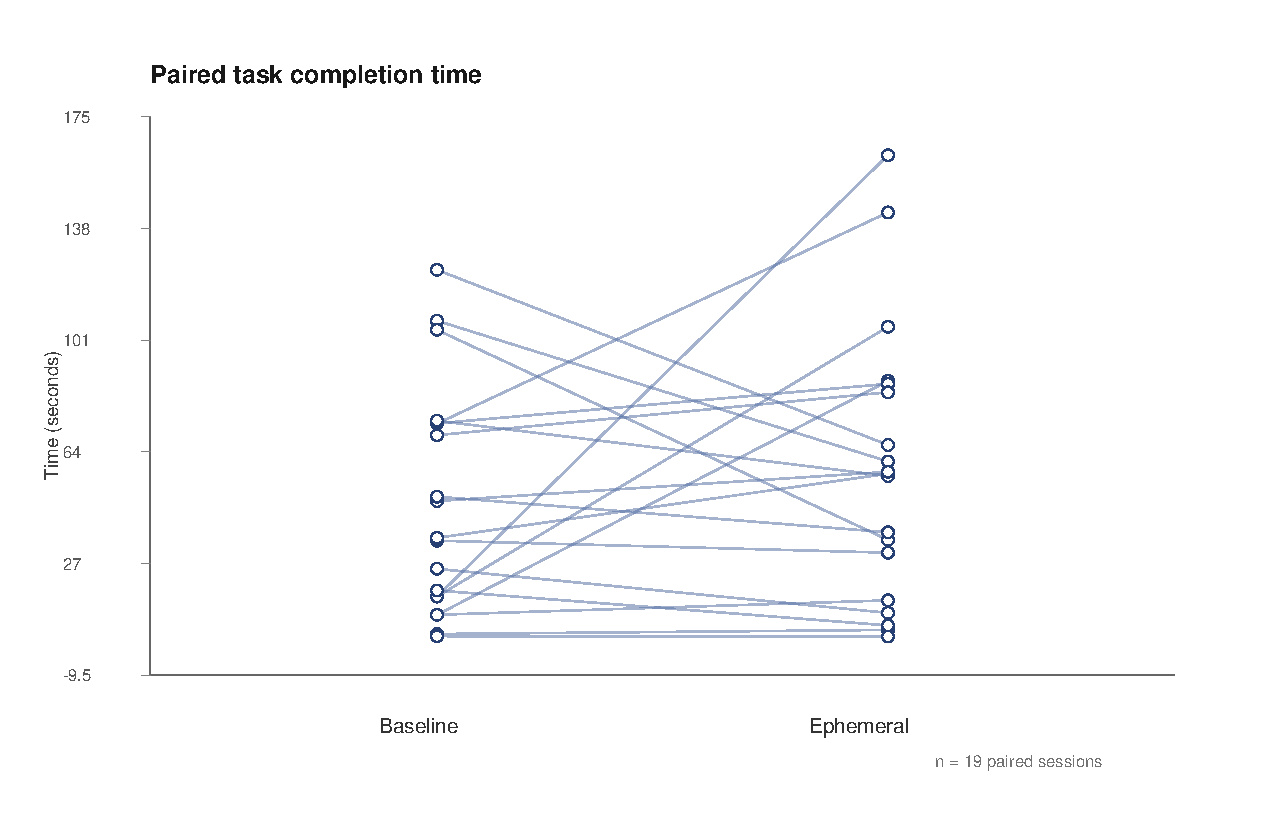
\includegraphics[width=0.65\textwidth]{graphics/results-completion-time.pdf}
    \caption{Paired comparison of task completion time (seconds) between the baseline and ephemeral conditions. Each line connects the same participant across conditions.}
    \label{fig:completion-time}
\end{figure}

\subsection{Interaction Count}

% SQL — interaction count per condition:
% SELECT t.condition,
%        count(*) AS n,
%        round(avg(t.interaction_count), 1) AS mean_interactions,
%        percentile_cont(0.5) WITHIN GROUP (ORDER BY t.interaction_count) AS median_interactions,
%        percentile_cont(0.25) WITHIN GROUP (ORDER BY t.interaction_count) AS q1,
%        percentile_cont(0.75) WITHIN GROUP (ORDER BY t.interaction_count) AS q3
% FROM trials t
% JOIN ( <valid participants subquery> ) v ON v.id = t.participant_id
% WHERE t.completed = true
% GROUP BY t.condition;
%
% SQL — paired interaction data for Wilcoxon (export as CSV):
% SELECT
%   b.participant_id,
%   b.interaction_count AS baseline_interactions,
%   e.interaction_count AS ephemeral_interactions
% FROM trials b
% JOIN trials e ON e.participant_id = b.participant_id
%              AND e.condition = 'ephemeral'
% JOIN ( <valid participants subquery> ) v ON v.id = b.participant_id
% WHERE b.condition = 'baseline'
%   AND b.completed = true AND e.completed = true;

The total number of logged interactions per trial was used as a proxy for task effort. The median interaction count in the baseline condition was \GenIntBaselineMdn{} (IQR: \GenIntBaselineIqr{}), compared to \GenIntEphemeralMdn{} (IQR: \GenIntEphemeralIqr{}) in the ephemeral condition. A Wilcoxon signed-rank test \GenIntWilcoxonResult{} ($W = \GenIntW$, $p = \GenIntP$, $r = \GenIntR$).

\thesistodo{Clarify that the ephemeral condition includes support-related interactions such as support shown and support dismissed. If the interaction count is higher, explain whether this reflects greater task effort or simply the extra steps introduced by the support layer.}

\begin{figure}[htbp]
    \centering
    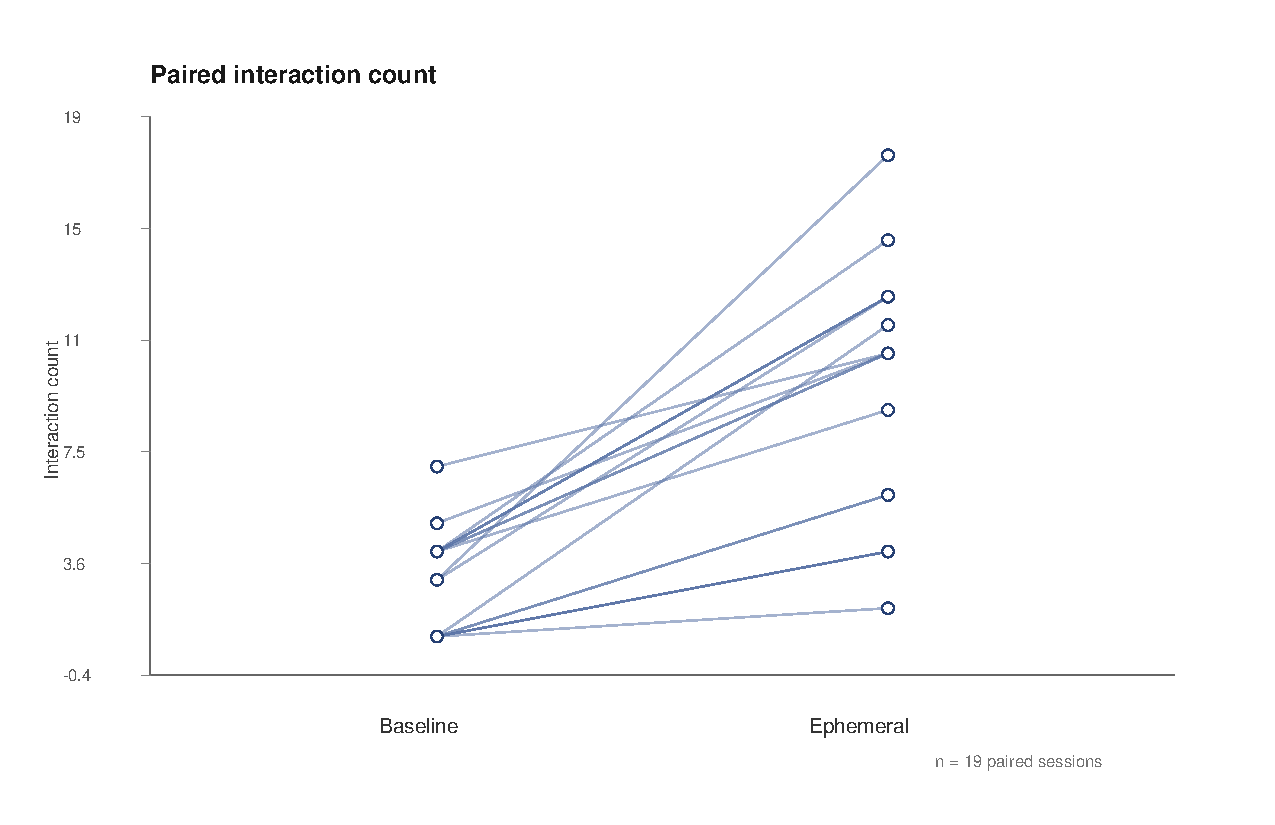
\includegraphics[width=0.65\textwidth]{graphics/results-interaction-count.pdf}
    \caption{Paired comparison of interaction count between the baseline and ephemeral conditions.}
    \label{fig:interaction-count}
\end{figure}

\subsection{Subjective Ratings}

% SQL — post-trial Likert ratings per condition:
% SELECT t.condition, qr.question_key,
%        count(*) AS n,
%        percentile_cont(0.5) WITHIN GROUP (ORDER BY qr.response_value::int) AS median_rating,
%        percentile_cont(0.25) WITHIN GROUP (ORDER BY qr.response_value::int) AS q1,
%        percentile_cont(0.75) WITHIN GROUP (ORDER BY qr.response_value::int) AS q3
% FROM questionnaire_responses qr
% JOIN trials t ON t.id = qr.trial_id
% JOIN ( <valid participants subquery> ) v ON v.id = qr.participant_id
% WHERE qr.question_key IN ('helpfulness', 'intrusiveness', 'control')
% GROUP BY t.condition, qr.question_key
% ORDER BY qr.question_key, t.condition;
%
% SQL — paired Likert data for Wilcoxon (export as CSV):
% SELECT
%   b_qr.participant_id,
%   b_qr.question_key,
%   b_qr.response_value::int AS baseline_rating,
%   e_qr.response_value::int AS ephemeral_rating
% FROM questionnaire_responses b_qr
% JOIN trials b_t ON b_t.id = b_qr.trial_id AND b_t.condition = 'baseline'
% JOIN trials e_t ON e_t.participant_id = b_t.participant_id
%                AND e_t.condition = 'ephemeral'
% JOIN questionnaire_responses e_qr ON e_qr.trial_id = e_t.id
%                                  AND e_qr.question_key = b_qr.question_key
% JOIN ( <valid participants subquery> ) v ON v.id = b_qr.participant_id
% WHERE b_qr.question_key IN ('helpfulness', 'intrusiveness', 'control');

After each trial, participants rated the interface on three dimensions using a seven-point Likert scale. Table~\ref{tab:likert} summarises the results.

\begin{table}[htbp]
    \centering
    \caption{Post-trial subjective ratings (7-point Likert scale, 1 = low, 7 = high).}
    \label{tab:likert}
    \begin{tabular}{@{}lccccc@{}}
        \toprule
        Measure & \multicolumn{2}{c}{Baseline} & \multicolumn{2}{c}{Ephemeral} & Wilcoxon \\
        \cmidrule(lr){2-3} \cmidrule(lr){4-5}
        & Mdn & IQR & Mdn & IQR & $p$ \\
        \midrule
        Helpfulness & \GenLikertHelpfulnessBaselineMdn{} & \GenLikertHelpfulnessBaselineIqr{} & \GenLikertHelpfulnessEphemeralMdn{} & \GenLikertHelpfulnessEphemeralIqr{} & \GenLikertHelpfulnessP{} \\
        Intrusiveness & \GenLikertIntrusivenessBaselineMdn{} & \GenLikertIntrusivenessBaselineIqr{} & \GenLikertIntrusivenessEphemeralMdn{} & \GenLikertIntrusivenessEphemeralIqr{} & \GenLikertIntrusivenessP{} \\
        Perceived control & \GenLikertControlBaselineMdn{} & \GenLikertControlBaselineIqr{} & \GenLikertControlEphemeralMdn{} & \GenLikertControlEphemeralIqr{} & \GenLikertControlP{} \\
        \bottomrule
    \end{tabular}
\end{table}

\thesistodo{Add one short paragraph per measure interpreting direction and significance. Cover whether the ephemeral condition was rated as more helpful, whether it felt more intrusive, and whether perceived control remained stable or changed.}

\begin{figure}[htbp]
    \centering
    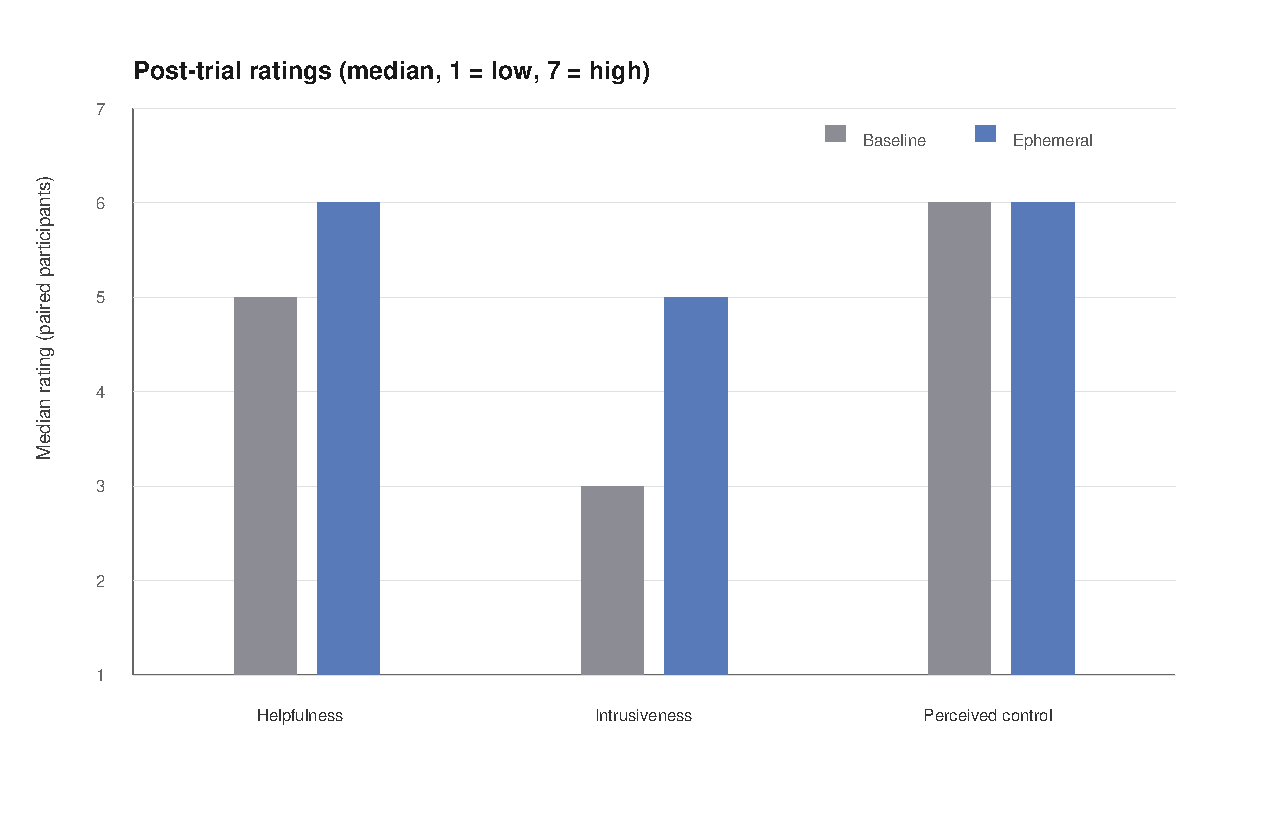
\includegraphics[width=0.75\textwidth]{graphics/results-likert-ratings.pdf}
    \caption{Median post-trial ratings by measure and condition (1 = low, 7 = high). Bars show the median rating across paired participants for each measure.}
    \label{fig:likert}
\end{figure}

\subsection{Overall Preference}

% SQL — final preference (raw A/B/same responses):
% SELECT qr.question_key, qr.response_value, count(*) AS n
% FROM questionnaire_responses qr
% JOIN ( <valid participants subquery> ) v ON v.id = qr.participant_id
% WHERE qr.trial_id IS NULL
%   AND qr.question_key IN ('final_preference', 'final_helpfulness',
%                           'final_intrusiveness', 'final_real_life')
% GROUP BY qr.question_key, qr.response_value
% ORDER BY qr.question_key, qr.response_value;
%
% SQL — final preference mapped to actual condition:
% SELECT
%   qr.question_key,
%   CASE
%     WHEN qr.response_value = 'same' THEN 'no_preference'
%     WHEN (qr.response_value = 'A' AND p.baseline_is_version_a)
%       OR (qr.response_value = 'B' AND NOT p.baseline_is_version_a)
%       THEN 'baseline'
%     ELSE 'ephemeral'
%   END AS actual_preference,
%   count(*) AS n
% FROM questionnaire_responses qr
% JOIN participants p ON p.id = qr.participant_id
% JOIN ( <valid participants subquery> ) v ON v.id = qr.participant_id
% WHERE qr.trial_id IS NULL
%   AND qr.question_key IN ('final_preference', 'final_helpfulness',
%                           'final_intrusiveness', 'final_real_life')
% GROUP BY qr.question_key, actual_preference
% ORDER BY qr.question_key, actual_preference;

After completing both trials, participants answered four forced-choice comparison questions. Responses were stored as Version~A or Version~B and mapped back to the actual experimental condition using each participant's counterbalancing assignment. Table~\ref{tab:preference} summarises the results.

\begin{table}[htbp]
    \centering
    \caption{Final comparative preference questions ($n = \GenNValid$).}
    \label{tab:preference}
    \begin{tabular}{@{}lccc@{}}
        \toprule
        Question & Baseline & Ephemeral & No preference \\
        \midrule
        Overall preference & \GenPrefOverallB{} & \GenPrefOverallE{} & \GenPrefOverallN{} \\
        More helpful & \GenPrefHelpB{} & \GenPrefHelpE{} & \GenPrefHelpN{} \\
        More intrusive & \GenPrefIntrB{} & \GenPrefIntrE{} & \GenPrefIntrN{} \\
        Real-life preference & \GenPrefLifeB{} & \GenPrefLifeE{} & \GenPrefLifeN{} \\
        \bottomrule
    \end{tabular}
\end{table}

\thesistodo{Run a binomial test for the overall preference question excluding no-preference responses, then report whether participants meaningfully favoured one condition.}

\subsection{Ephemeral Support Engagement}

% SQL — ephemeral-only support engagement summary:
% SELECT
%   count(DISTINCT te.trial_id) FILTER (WHERE te.event_type = 'support_triggered') AS trials_triggered,
%   count(DISTINCT te.trial_id) FILTER (WHERE te.event_type = 'support_requested') AS trials_requested,
%   count(DISTINCT te.trial_id) FILTER (WHERE te.event_type = 'support_shown') AS trials_shown,
%   count(DISTINCT te.trial_id) FILTER (WHERE te.event_type = 'support_used') AS trials_used,
%   count(DISTINCT te.trial_id) FILTER (WHERE te.event_type = 'support_dismissed') AS trials_dismissed,
%   count(DISTINCT te.trial_id) FILTER (WHERE te.event_type = 'support_ignored') AS trials_ignored,
%   count(DISTINCT te.trial_id) FILTER (WHERE te.event_type = 'support_inspect_expanded') AS trials_expanded
% FROM trial_events te
% JOIN trials t ON t.id = te.trial_id AND t.condition = 'ephemeral'
% JOIN ( <valid participants subquery> ) v ON v.id = te.participant_id;
%
% SQL — per-participant support event counts:
% SELECT
%   te.participant_id,
%   te.event_type,
%   count(*) AS event_count
% FROM trial_events te
% JOIN trials t ON t.id = te.trial_id AND t.condition = 'ephemeral'
% JOIN ( <valid participants subquery> ) v ON v.id = te.participant_id
% WHERE te.event_type IN ('support_triggered', 'support_requested',
%                         'support_shown', 'support_used',
%                         'support_dismissed', 'support_ignored',
%                         'support_inspect_expanded')
% GROUP BY te.participant_id, te.event_type
% ORDER BY te.participant_id, te.event_type;
%
% SQL — fallback rate:
% SELECT
%   count(*) AS total_generations,
%   count(*) FILTER (WHERE (output->>'usedFallback')::boolean = true) AS fallback_count,
%   round(100.0 * count(*) FILTER (WHERE (output->>'usedFallback')::boolean = true)
%         / count(*), 1) AS fallback_pct
% FROM support_outputs so
% JOIN trials t ON t.id = so.trial_id
% JOIN ( <valid participants subquery> ) v ON v.id = t.participant_id;

To interpret the behavioural and subjective results in context, this subsection reports how participants actually interacted with the ephemeral support layer. These measures apply only to the ephemeral condition.

Of the \GenNValid{} participants who completed the ephemeral trial, support was triggered or explicitly requested in \GenEngNTriggered{} cases (\GenEngPctTriggered{}\%). Once shown, support was actively used (applied or confirmed) in \GenEngNUsed{} cases, dismissed without use in \GenEngNDismissed{} cases, and ignored entirely in \GenEngNIgnored{} cases. \GenEngNExpanded{} participants expanded the support for further detail. The support generation pipeline produced \GenEngTotalGen{} specifications in total, of which \GenEngFallbackCount{} (\GenEngFallbackPct{}\%) fell back to the deterministic fallback because the generated output failed validation.

\thesistodo{Interpret the engagement pattern. If most participants used the support, say the main results are directly interpretable. If many dismissed or ignored it, note that the measured effects may either understate the potential of ephemeral assistance or indicate that the support was not perceived as useful.}

\subsection{Summary of Findings}

\thesistodo{Write a short factual summary of the findings in 4 to 6 sentences. Cover completion rate, completion time, interaction count, subjective ratings, preference, and engagement, and use it as a bridge into the discussion.}

Table~\ref{tab:results-summary} provides an overview of all primary outcome measures.

\begin{table}[htbp]
    \centering
    \caption{Summary of primary outcome measures across conditions.}
    \label{tab:results-summary}
    \begin{tabular}{@{}llll@{}}
        \toprule
        Measure & Baseline & Ephemeral & $p$ \\
        \midrule
        Completion rate & \GenSumCompPctB{}\% & \GenSumCompPctE{}\% & \GenSumMcNemarP{} \\
        Completion time (Mdn, s) & \GenSumTimeBMdn{} & \GenSumTimeEMdn{} & \GenSumTimeP{} \\
        Interaction count (Mdn) & \GenSumIntBMdn{} & \GenSumIntEMdn{} & \GenSumIntP{} \\
        Helpfulness (Mdn) & \GenSumHelpBMdn{} & \GenSumHelpEMdn{} & \GenSumHelpP{} \\
        Intrusiveness (Mdn) & \GenSumIntrBMdn{} & \GenSumIntrEMdn{} & \GenSumIntrP{} \\
        Perceived control (Mdn) & \GenSumCtrlBMdn{} & \GenSumCtrlEMdn{} & \GenSumCtrlP{} \\
        Overall preference & \multicolumn{2}{c}{\GenSumPrefOverall{}} & \GenSumPrefOverallP{} \\
        \bottomrule
    \end{tabular}
\end{table}

\pagestyle{fancy} 
\section{Discussion}

This is your discussion text

- Talk about the data u got and what can be inferred
- Compare with other sources and what they got and how they differ
\pagestyle{fancy} 
\section{Future Work}\label{sec:future-work}

The present evaluation is intentionally narrow: one scenario, one operationalisation of the framework, and a remote, self-paced procedure. The directions below follow from that scope and from what the artifact already suggests about where ephemeral, task-scoped support may be most informative next.

\subsection{Broader scenarios and user populations}

The study used a single presentation-refinement workflow. Ephemeral support is unlikely to matter equally in every domain. Prior work like with BISCUIT \parencite{Cheng2024Biscuit} suggest that ephemeral interface scaffolds work well with computational notebooks for data science exploration where they can steer intermediate output. Thus, it provides a useful contrast to this thesis where it focused on specific technical workflow, whereas this projects focuses if ephemeral support can add value in conventional interfaces for a larger user demographic. The current results show that less focus should be made on broad domains and more on the workflow properties of interruption tolerance, consequence of error, and whether the assisted action is a bounded local refinement rather than a high-stakes commitment. The most interesting scenarios to test next would be technical refinement tasks through several iterations. For example, when a designer wants to tweak the layout or hierarchy of their designs or a data scientist adjusting the parameters of a machine learning model they both require real time feedback from their actions. The same reasoning indicates significant limitations regarding the appropriateness of ephemeral support. Within heavily regulated areas like finance, law, or healthcare ephemeral generative UI may not be an ideal use case as those scenarios. This is as they require stricter predictability, traceability, and accountability than low risk situations like adding tasks to a todo list, even if it's proven useful for refinement tasks. This possibility also aligns with the claim that adaptive support could be the most valuable when traditional interfaces struggle to accommodate varying user needs across different contexts \parencite{Bieniek2024GenerativeAI,Tambi2020GenerativeBanking}. The next step is to evaluate the framework across several workflows that differ in interruption tolerance, consequence of error, task significance, technical complexity, familiarity with the application, and degree of regulatory constraint. It would clarify situations when ephemeral support is genuinely helpful for end users or if it gives irrelevant guidance for a clear user workflow.

\subsection{Deeper evaluation methods}


Increasing the number of completions would make the statistics more reliable, but it wouldn't explain why participants acted the way they did or how they understood the support. Another direction would be to do in depth evaluation in focus groups where a researcher can observe the misunderstanding of triggers and emotional reactions of the participants that questionnaires can only partially capture. Using both controlled experiments and focus groups could link specific design choices to real friction and also to how intrusive or controllable the support felt.

\subsection{Richer ephemeral component catalogues}

The evaluation artifact deliberately used a constrained set of ephemeral UI components so that conditions remained comparable and the study remained feasible within the capstone timeline. The underlying framework could support a wider catalogue: more varied layouts, stronger personalisation of content and tone based on the user's profile, role, or prior behaviour, and more expressive temporary interaction patterns than were deployed here. Exploring that wider design space would also connect more directly to the broader literature, which frames generative interfaces in terms of adaptive, context-sensitive interaction structures while also warning that flexibility can come at the cost of predictability and user control \parencite{Bieniek2024GenerativeAI}. At the same time, the foundational logic of ephemerality suggests that temporary interface elements should appear only when relevant and should recede without leaving persistent clutter \parencite{Doring2013EphemeralUI}. Expanding the catalogue therefore raises its own research questions about how to preserve predictability and user agency when surface behaviour varies more widely, and how to evaluate more personalised variants without confounding condition effects with implementation novelty. Future work could treat catalogue design as a first-class object of study: progressive disclosure of complexity, user-tunable boundaries for ephemerality, and systematic comparison of a small number of high-diversity implementations against a stable baseline.

\pagestyle{fancy} 
\section{Conclusion}

This thesis asked how ephemeral, task-scoped generative UI components can be designed to improve existing applications without disrupting the user experience. To address that question, it developed a conceptual framework for ephemeral support, implemented the framework in an experimental web artifact, and evaluated the artifact against a persistent baseline in a within-subjects user study. The evaluation provides a qualified answer to that question: ephemeral support can be introduced in a bounded way that preserves users' sense of control, but the implementation tested here did not produce clear performance gains without also introducing additional intrusiveness.

Across the study measures, the ephemeral condition showed a slightly higher task completion rate, although that difference was not statistically significant, and a significantly higher perceived helpfulness rating. Completion time likewise did not improve. By contrast, interaction count increased substantially and perceived intrusiveness increased significantly, while perceived control remained stable and overall preference did not clearly favour either condition. These findings suggest that the main contribution of the ephemeral layer in this prototype was not faster task execution, but a clearer sense of perceived support that came with a noticeable interaction cost.

The thesis's individual contribution lies not only in evaluating ephemeral support as an idea, but in operationalising it through a constrained component-specification model, a validation pipeline for generated interface specifications, a bounded ephemeral overlay approach that preserves host-interface continuity, and an interactive survey artifact that makes empirical evaluation possible.

The broader implication is that ephemeral, task-scoped generative UI remains a promising design direction, but its value depends on more than simply making support temporary. For such support to improve existing applications in practice, it must appear at the right moment, be immediately legible, and offer enough value that users choose to engage with it rather than dismiss it. The present findings support a narrower conclusion than claiming a best-fit domain such as productivity work in general or technical design work specifically. The safer conclusion is that ephemeral support is most credible for bounded, low-consequence subtasks within stable interfaces, particularly where lightweight contextual guidance may help and the cost of interruption remains manageable. The framework proposed in this thesis helps define those boundaries, while the study shows both their promise and their current limits. Technical iterative-refinement settings, such as design exploration or parameter tuning with immediate feedback, are plausible next contexts for evaluation, but they remain future directions rather than validated conclusions from the present study. Future work should therefore test richer scenarios, broader user populations, and more refined support behaviours in order to determine when ephemeral generative assistance becomes not only possible within stable interfaces, but meaningfully beneficial.

\begin{appendices}

\section{Appendix}

This appendix documents the key analysis steps used to transform the study database into the statistics, figures, and thesis-ready result values reported in Section~4. Because the examiner cannot assume access to the full repository, the appendix includes selected code excerpts that demonstrate the core logic of participant selection, statistical testing, figure generation, and LaTeX value generation. The excerpts are representative rather than exhaustive: they are intended to show how the analysis was implemented, not to reproduce every utility function in full.

\subsection{Analysis Pipeline Overview}

The analysis workflow was implemented as a small Bun-based pipeline. Rather than copying values manually into the thesis, the pipeline exported study data from PostgreSQL, computed the required descriptive and inferential statistics, generated the figure PDFs used in the results chapter, and wrote the LaTeX macro file that supplied numeric values to the manuscript. This structure reduced transcription risk and kept the reported values tied to executable analysis code.

The pipeline can be summarised in four stages:

\begin{enumerate}
    \item export the required study data to intermediate CSV files,
    \item compute the paired statistical tests used in the results chapter,
    \item generate the PDF figures included in the results chapter, and
    \item regenerate the LaTeX macros that populate reported values throughout Section~4.
\end{enumerate}

This means that the values appearing in the results chapter were derived from the exported data rather than entered by hand. If the underlying database contents changed, rerunning the pipeline updated both the figures and the numeric placeholders used in the LaTeX source.

\subsection{Representative Analysis Listings}

The following listings were selected because they show the most thesis-relevant parts of the implementation: the rule used to determine the analysed sample, the paired non-parametric statistical test used for several outcomes, the generation of the main numeric figures, and the production of thesis-ready LaTeX commands.

\subsubsection{Participant Inclusion Logic}

Listing~\ref{lst:valid-participants} shows the reusable SQL filter used throughout the analysis. A participant was included only if they completed both task trials and answered all four final comparison questions. This ensured that all reported measures were computed from a consistent completer sample.

\begin{listing}[p]
\caption{SQL logic used to define the valid participant sample.}
\label{lst:valid-participants}
\begin{minted}[fontsize=\small,breaklines]{sql}
WITH valid_participants AS (
  SELECT p.id, p.age_range, p.occupation,
         p.web_app_familiarity, p.ai_tool_familiarity,
         p.baseline_is_version_a
  FROM participants p
  WHERE (SELECT count(*) FROM trials t
         WHERE t.participant_id = p.id AND t.completed = true) = 2
    AND (SELECT count(DISTINCT question_key)
         FROM questionnaire_responses qr
         WHERE qr.participant_id = p.id
           AND qr.trial_id IS NULL
           AND qr.question_key IN (
             'final_preference',
             'final_helpfulness',
             'final_intrusiveness',
             'final_real_life'
           )) = 4
)
SELECT count(*) AS valid_completed
FROM valid_participants;
\end{minted}
\end{listing}

\subsubsection{Paired Statistical Testing}

Listing~\ref{lst:wilcoxon} shows the central implementation of the Wilcoxon signed-rank test used for paired completion time, interaction count, and post-trial Likert outcomes. The function removes zero differences, ranks the remaining paired differences by magnitude, computes the smaller rank sum $W$, and then uses an exact p-value for small samples or a normal approximation for larger ones. This matched the within-subjects design and the small paired sample available in the study.

\begin{listing}[htbp]
\caption{Core Wilcoxon signed-rank implementation used for paired outcomes.}
\label{lst:wilcoxon}
\begin{minted}[fontsize=\small,breaklines]{ts}
function wilcoxonSignedRank(
  baseline: number[],
  ephemeral: number[],
): { W: number; p: number; r: number; n: number } {
  const diffs: number[] = [];
  for (let i = 0; i < baseline.length; i++) {
    const d = ephemeral[i]! - baseline[i]!;
    if (d !== 0) diffs.push(d);
  }

  const n = diffs.length;
  if (n === 0) return { W: 0, p: 1, r: 0, n: 0 };

  const absDiffs = diffs.map((d) => ({ abs: Math.abs(d), sign: Math.sign(d) }));
  absDiffs.sort((a, b) => a.abs - b.abs);

  const ranks: number[] = [];
  let i = 0;
  while (i < absDiffs.length) {
    let j = i;
    while (j < absDiffs.length && absDiffs[j]!.abs === absDiffs[i]!.abs) j++;
    const avgRank = (i + 1 + j) / 2;
    for (let k = i; k < j; k++) ranks.push(avgRank);
    i = j;
  }

  let wPlus = 0;
  let wMinus = 0;
  for (let k = 0; k < n; k++) {
    if (absDiffs[k]!.sign > 0) wPlus += ranks[k]!;
    else wMinus += ranks[k]!;
  }

  const W = Math.min(wPlus, wMinus);
  const maxW = (n * (n + 1)) / 2;
  const p = n <= 25 ? wilcoxonExactP(W, n) : wilcoxonApproxP(W, n);
  const r = 1 - (2 * W) / maxW;

  return { W, p: Math.min(p, 1), r: Math.abs(r), n };
}
\end{minted}
\end{listing}

\subsubsection{Figure Generation}

Listing~\ref{lst:paired-plot} shows the core drawing loop used to produce the paired numeric plots for completion time and interaction count. Each participant contributes one baseline value and one ephemeral value, and the script draws a line connecting the two observations so that the within-participant change is visible directly in the figure.

\begin{listing}[htbp]
\caption{Core paired-plot drawing logic used for numeric result figures.}
\label{lst:paired-plot}
\begin{minted}[fontsize=\small,breaklines]{ts}
const baselineVals = rows.map((r) => Number(r[opts.baselineKey]));
const ephemeralVals = rows.map((r) => Number(r[opts.ephemeralKey]));

for (let i = 0; i < rows.length; i++) {
  const b = baselineVals[i]!;
  const e = ephemeralVals[i]!;
  if (Number.isNaN(b) || Number.isNaN(e)) continue;
  const y1 = yToPdf(b, minY, maxY, chartBottom, chartTop);
  const y2 = yToPdf(e, minY, maxY, chartBottom, chartTop);
  page.drawLine({
    start: { x: xLeft, y: y1 },
    end: { x: xRight, y: y2 },
    thickness: 0.8,
    color: lineColor,
    opacity: 0.55,
  });
}

for (let i = 0; i < rows.length; i++) {
  const b = baselineVals[i]!;
  const e = ephemeralVals[i]!;
  if (Number.isNaN(b) || Number.isNaN(e)) continue;
  const y1 = yToPdf(b, minY, maxY, chartBottom, chartTop);
  const y2 = yToPdf(e, minY, maxY, chartBottom, chartTop);
  page.drawCircle({ x: xLeft, y: y1, size: 2.8, borderColor: pointColor });
  page.drawCircle({ x: xRight, y: y2, size: 2.8, borderColor: pointColor });
}
\end{minted}
\end{listing}

\subsubsection{Thesis-Ready Value Generation}

Listing~\ref{lst:latex-macros} shows how the final numerical outputs were converted into LaTeX commands. Instead of entering p-values, medians, and percentages manually into the thesis text, the script generated commands such as \verb|\GenTimeP| and \verb|\GenCompPctBaseline|. The results chapter then imported these commands directly, ensuring that the prose, tables, and summary values all used the same generated source.

\begin{listing}[htbp]
\caption{Generation of LaTeX commands used throughout the results chapter.}
\label{lst:latex-macros}
\begin{minted}[fontsize=\small,breaklines]{ts}
const lines: string[] = [
  "% AUTO-GENERATED by analysis/generate-results-tex.ts -- do not edit by hand.",
  "% Regenerate: bun run gen-tex",
  "",
];

cmd(lines, "GenNTotal", String(s.overview.totalAccessed));
cmd(lines, "GenNValid", String(v));
cmd(lines, "GenCompPctBaseline", s.completion.pctBaseline.toFixed(1));
cmd(lines, "GenCompPctEphemeral", s.completion.pctEphemeral.toFixed(1));
cmd(lines, "GenCompMcNemarP", fmtP(s.completion.mcnemarP));

const tw = s.time.wilcoxon;
cmd(lines, "GenTimeBaselineMdn", safeFixed(s.time.baselineMdn, 1));
cmd(lines, "GenTimeEphemeralMdn", safeFixed(s.time.ephemeralMdn, 1));
cmd(lines, "GenTimeP", fmtP(tw?.p ?? null));

writeFileSync(OUT_TEX, lines.join("\n") + "\n", "utf-8");
\end{minted}
\end{listing}

\subsection{Local Generation Trace}\label{app:local-generation-trace}

In addition to the aggregate study dataset analysed in Section~4, I captured a local end-to-end validation trace from the implemented support pipeline itself. This trace was taken from the real \texttt{/api/support} route rather than the development-only playground endpoint, so it exercised the same request handling, prompt construction, validation stages, PostgreSQL persistence, and client-facing response path used during the study. The selected example below is the locally persisted record with \texttt{support\_output\_id = 103}, captured on 2026-04-04 during a hesitation-triggered \texttt{slides-outline-refine} trial.

\captionof{listing}{Condensed excerpt of a locally captured support-generation record.}
\label{lst:local-support-trace}
\inputminted[fontsize=\tiny,breaklines,breakanywhere]{json}{evidence/local-support-validation-2026-04-04.json}

\subsection{Participant Flow Screenshots}

Figures~\ref{fig:appendix-flow-1}--\ref{fig:appendix-flow-5} provide a chronological walkthrough of the participant-facing flow captured from the implemented artifact. These appendix figures complement the main-text interface screenshots by showing the sequence of states the participant moved through across the baseline trial, the ephemeral trial, and the final comparative questionnaire. One intervening transition capture that contained no visible interface content was omitted.

\begin{figure}[htbp]
    \centering
    \begin{subfigure}[t]{0.49\textwidth}
        \centering
        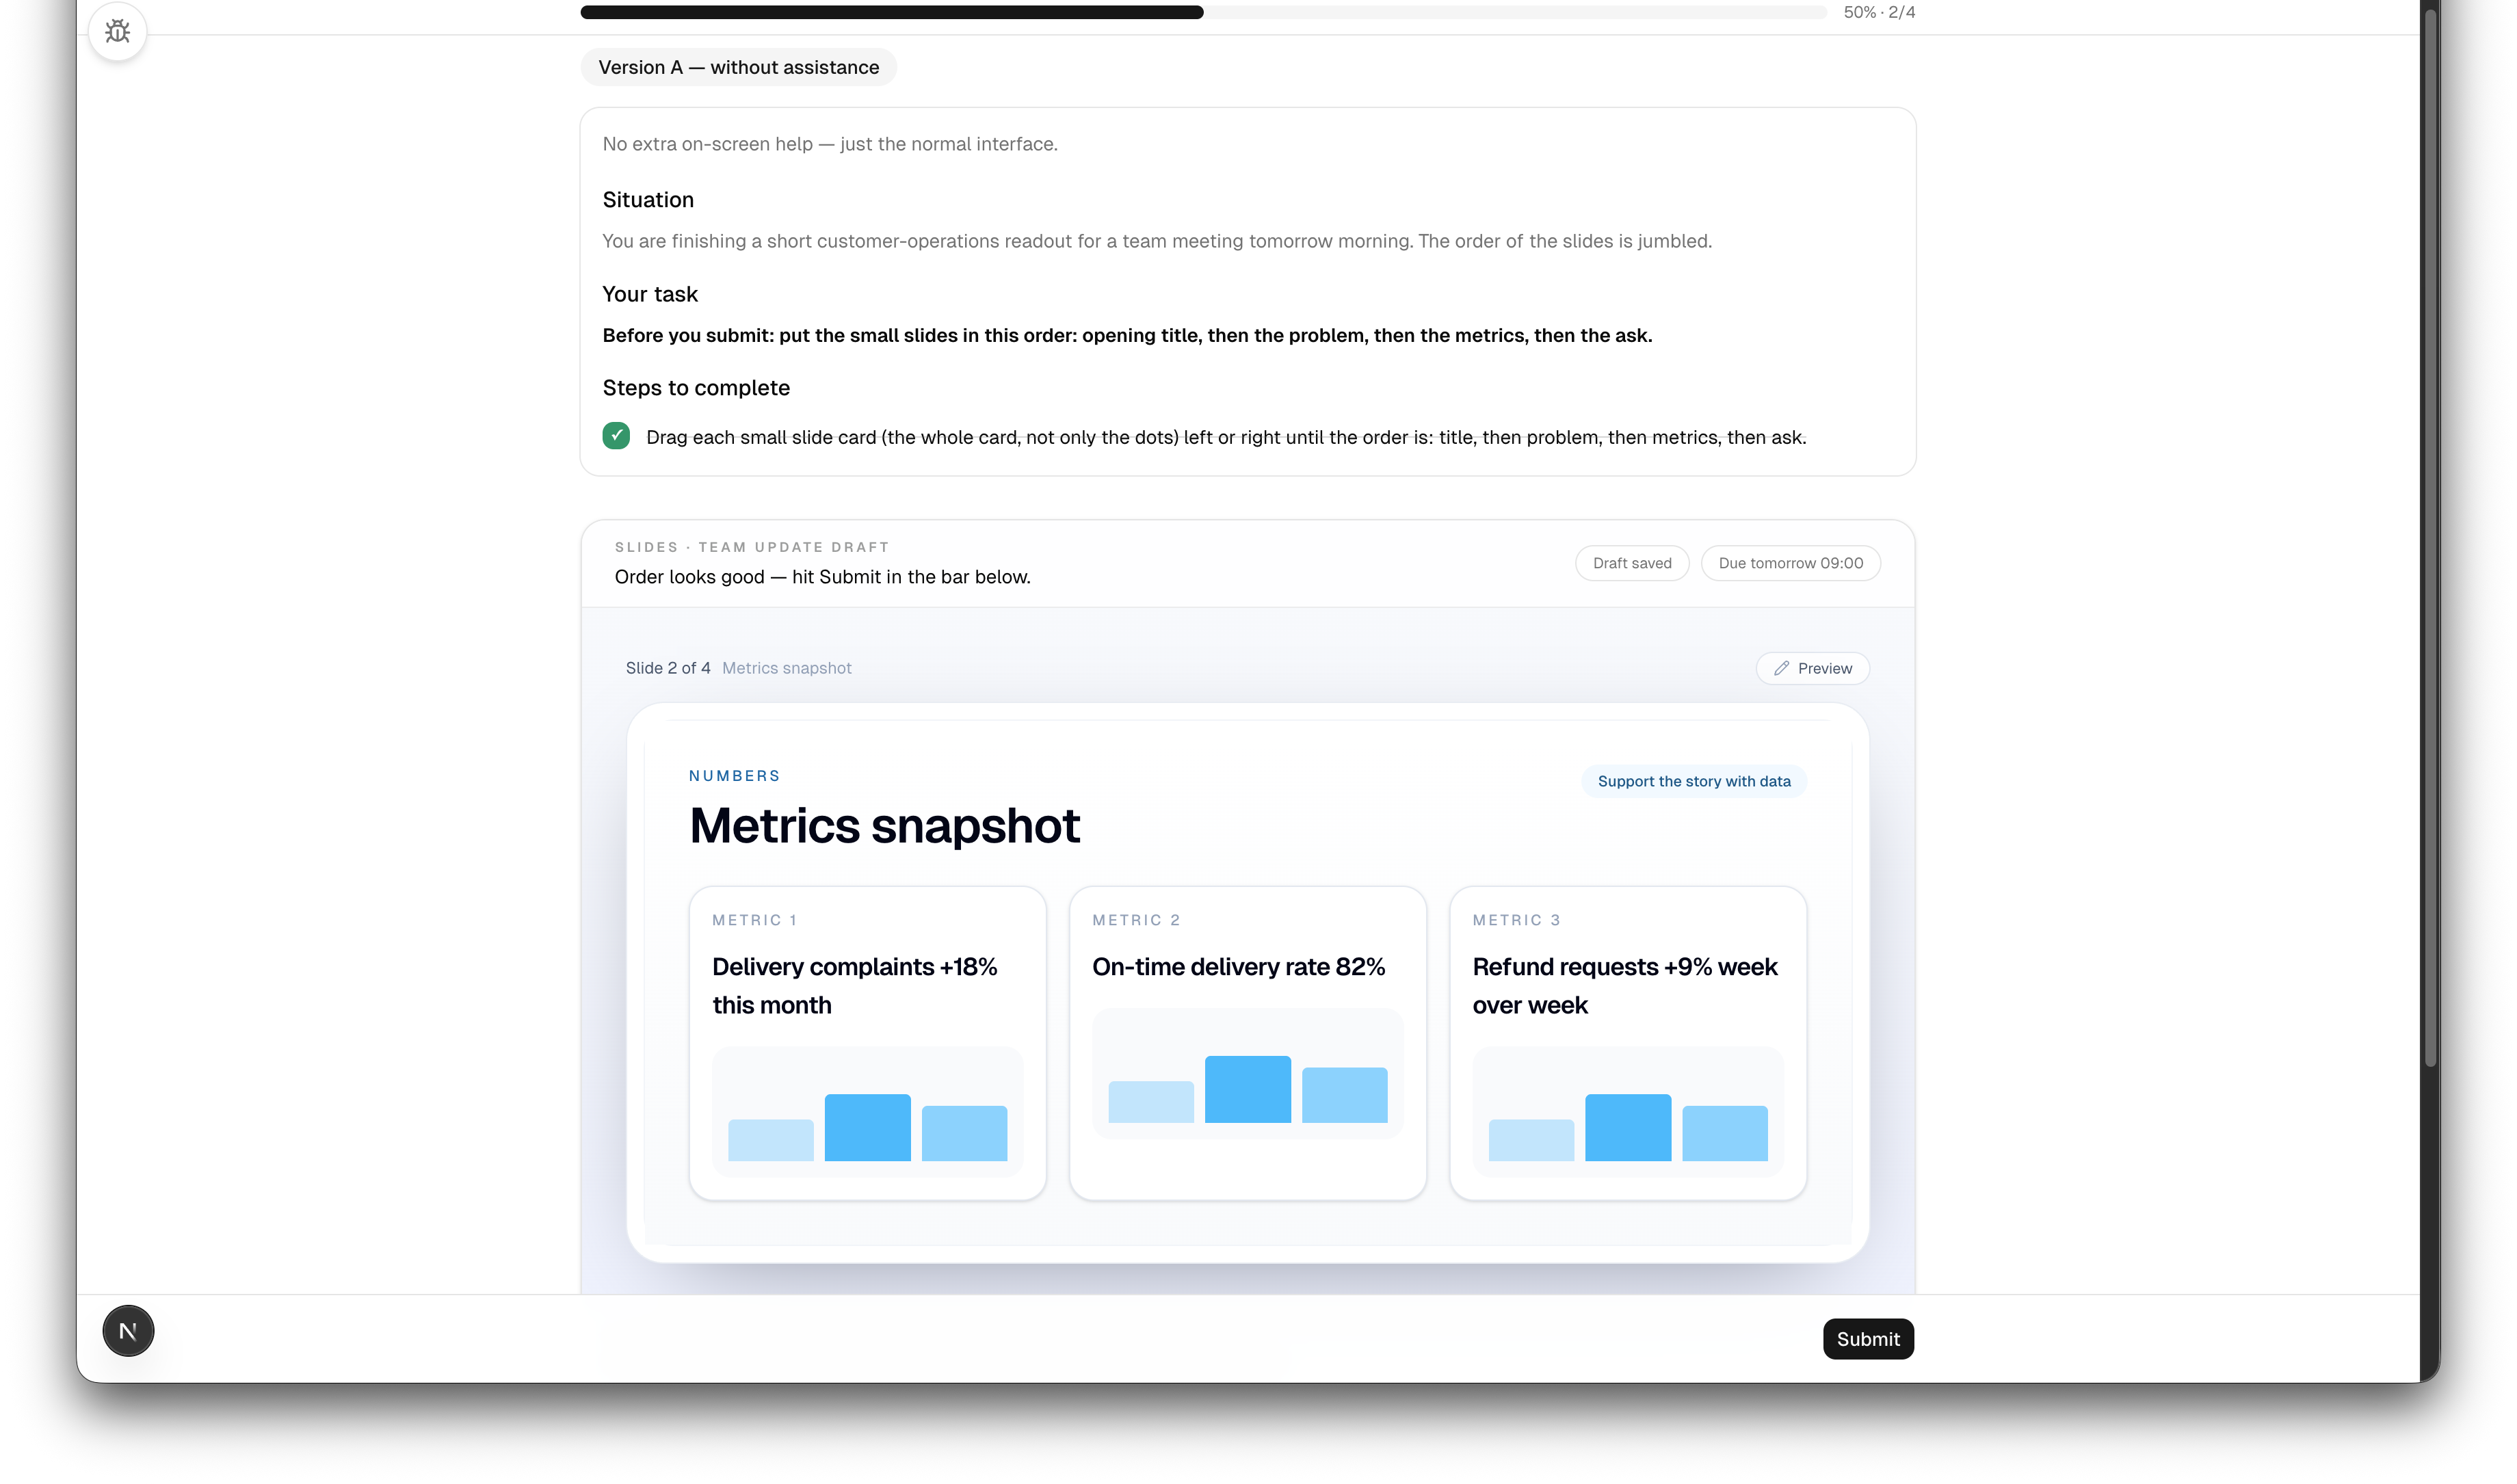
\includegraphics[width=\textwidth]{graphics/example-flow-1.png}
        \caption{Baseline trial with the plain interface visible and no temporary support.}
    \end{subfigure}
    \hfill
    \begin{subfigure}[t]{0.49\textwidth}
        \centering
        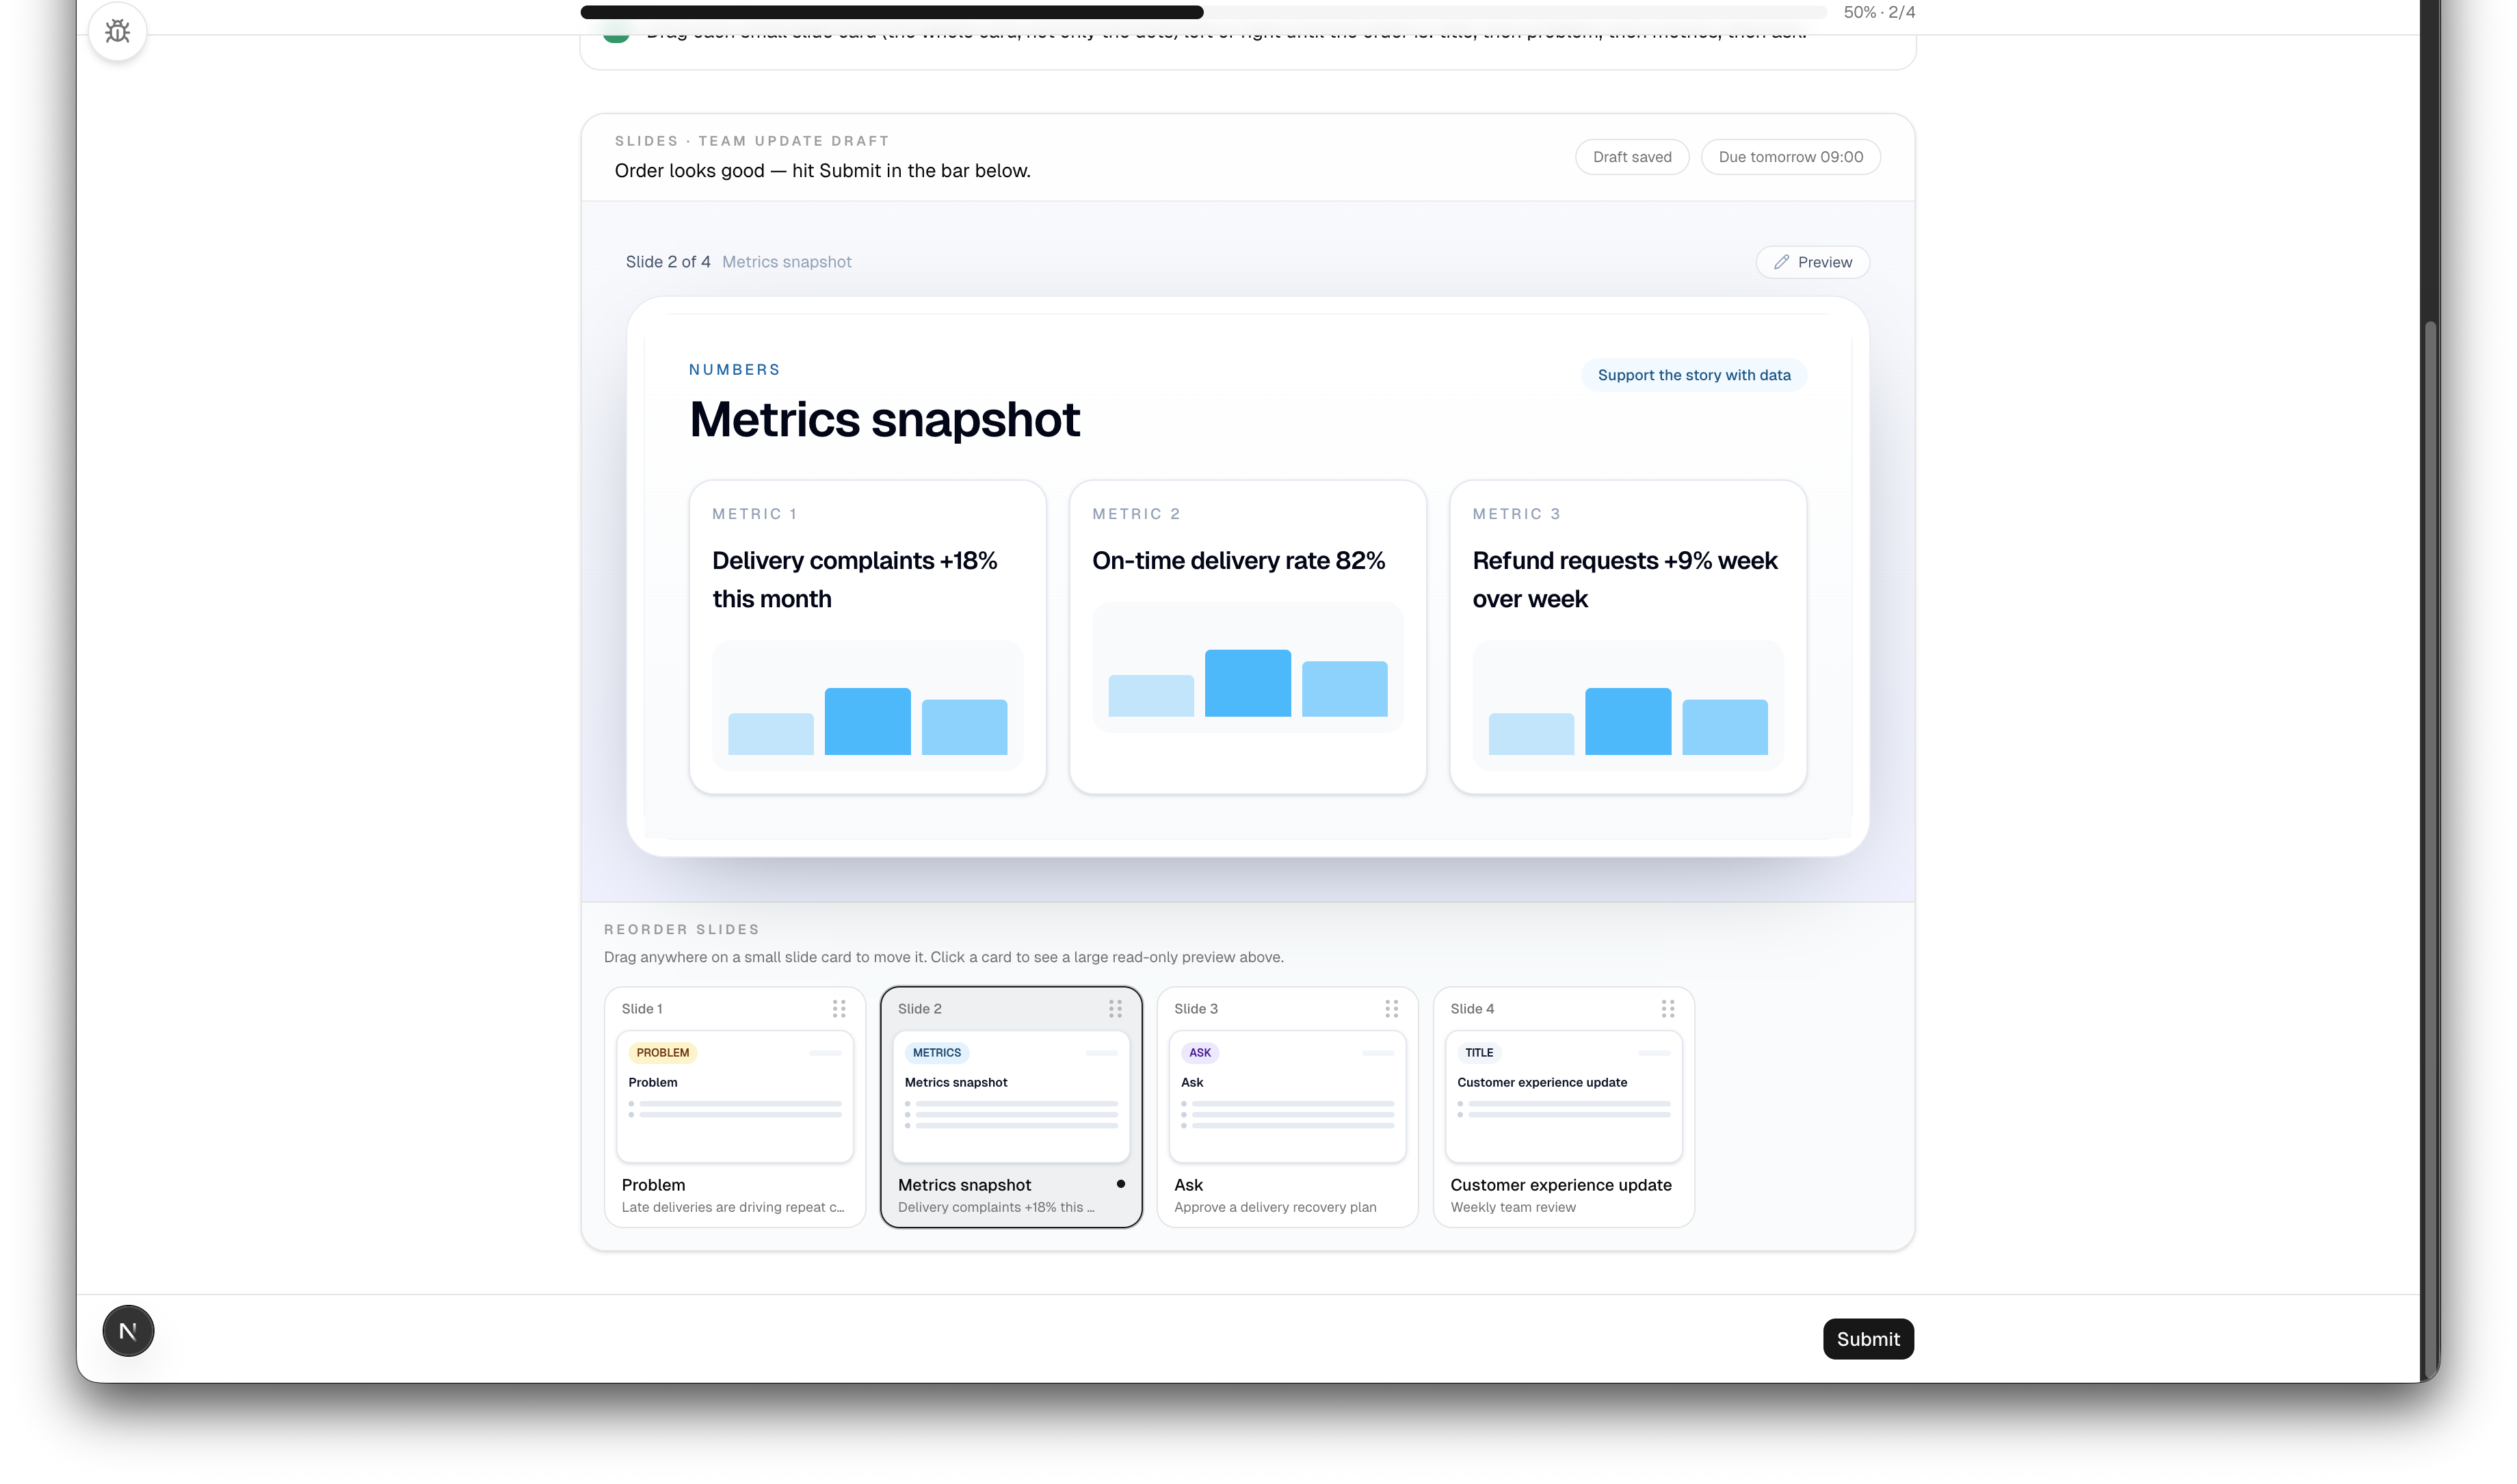
\includegraphics[width=\textwidth]{graphics/example-flow-2.png}
        \caption{Baseline task interaction while the participant reorders the slide strip.}
    \end{subfigure}
    \caption{Participant-flow walkthrough, part~1: baseline-condition task screens.}
    \label{fig:appendix-flow-1}
\end{figure}

\begin{figure}[htbp]
    \centering
    \begin{subfigure}[t]{0.49\textwidth}
        \centering
        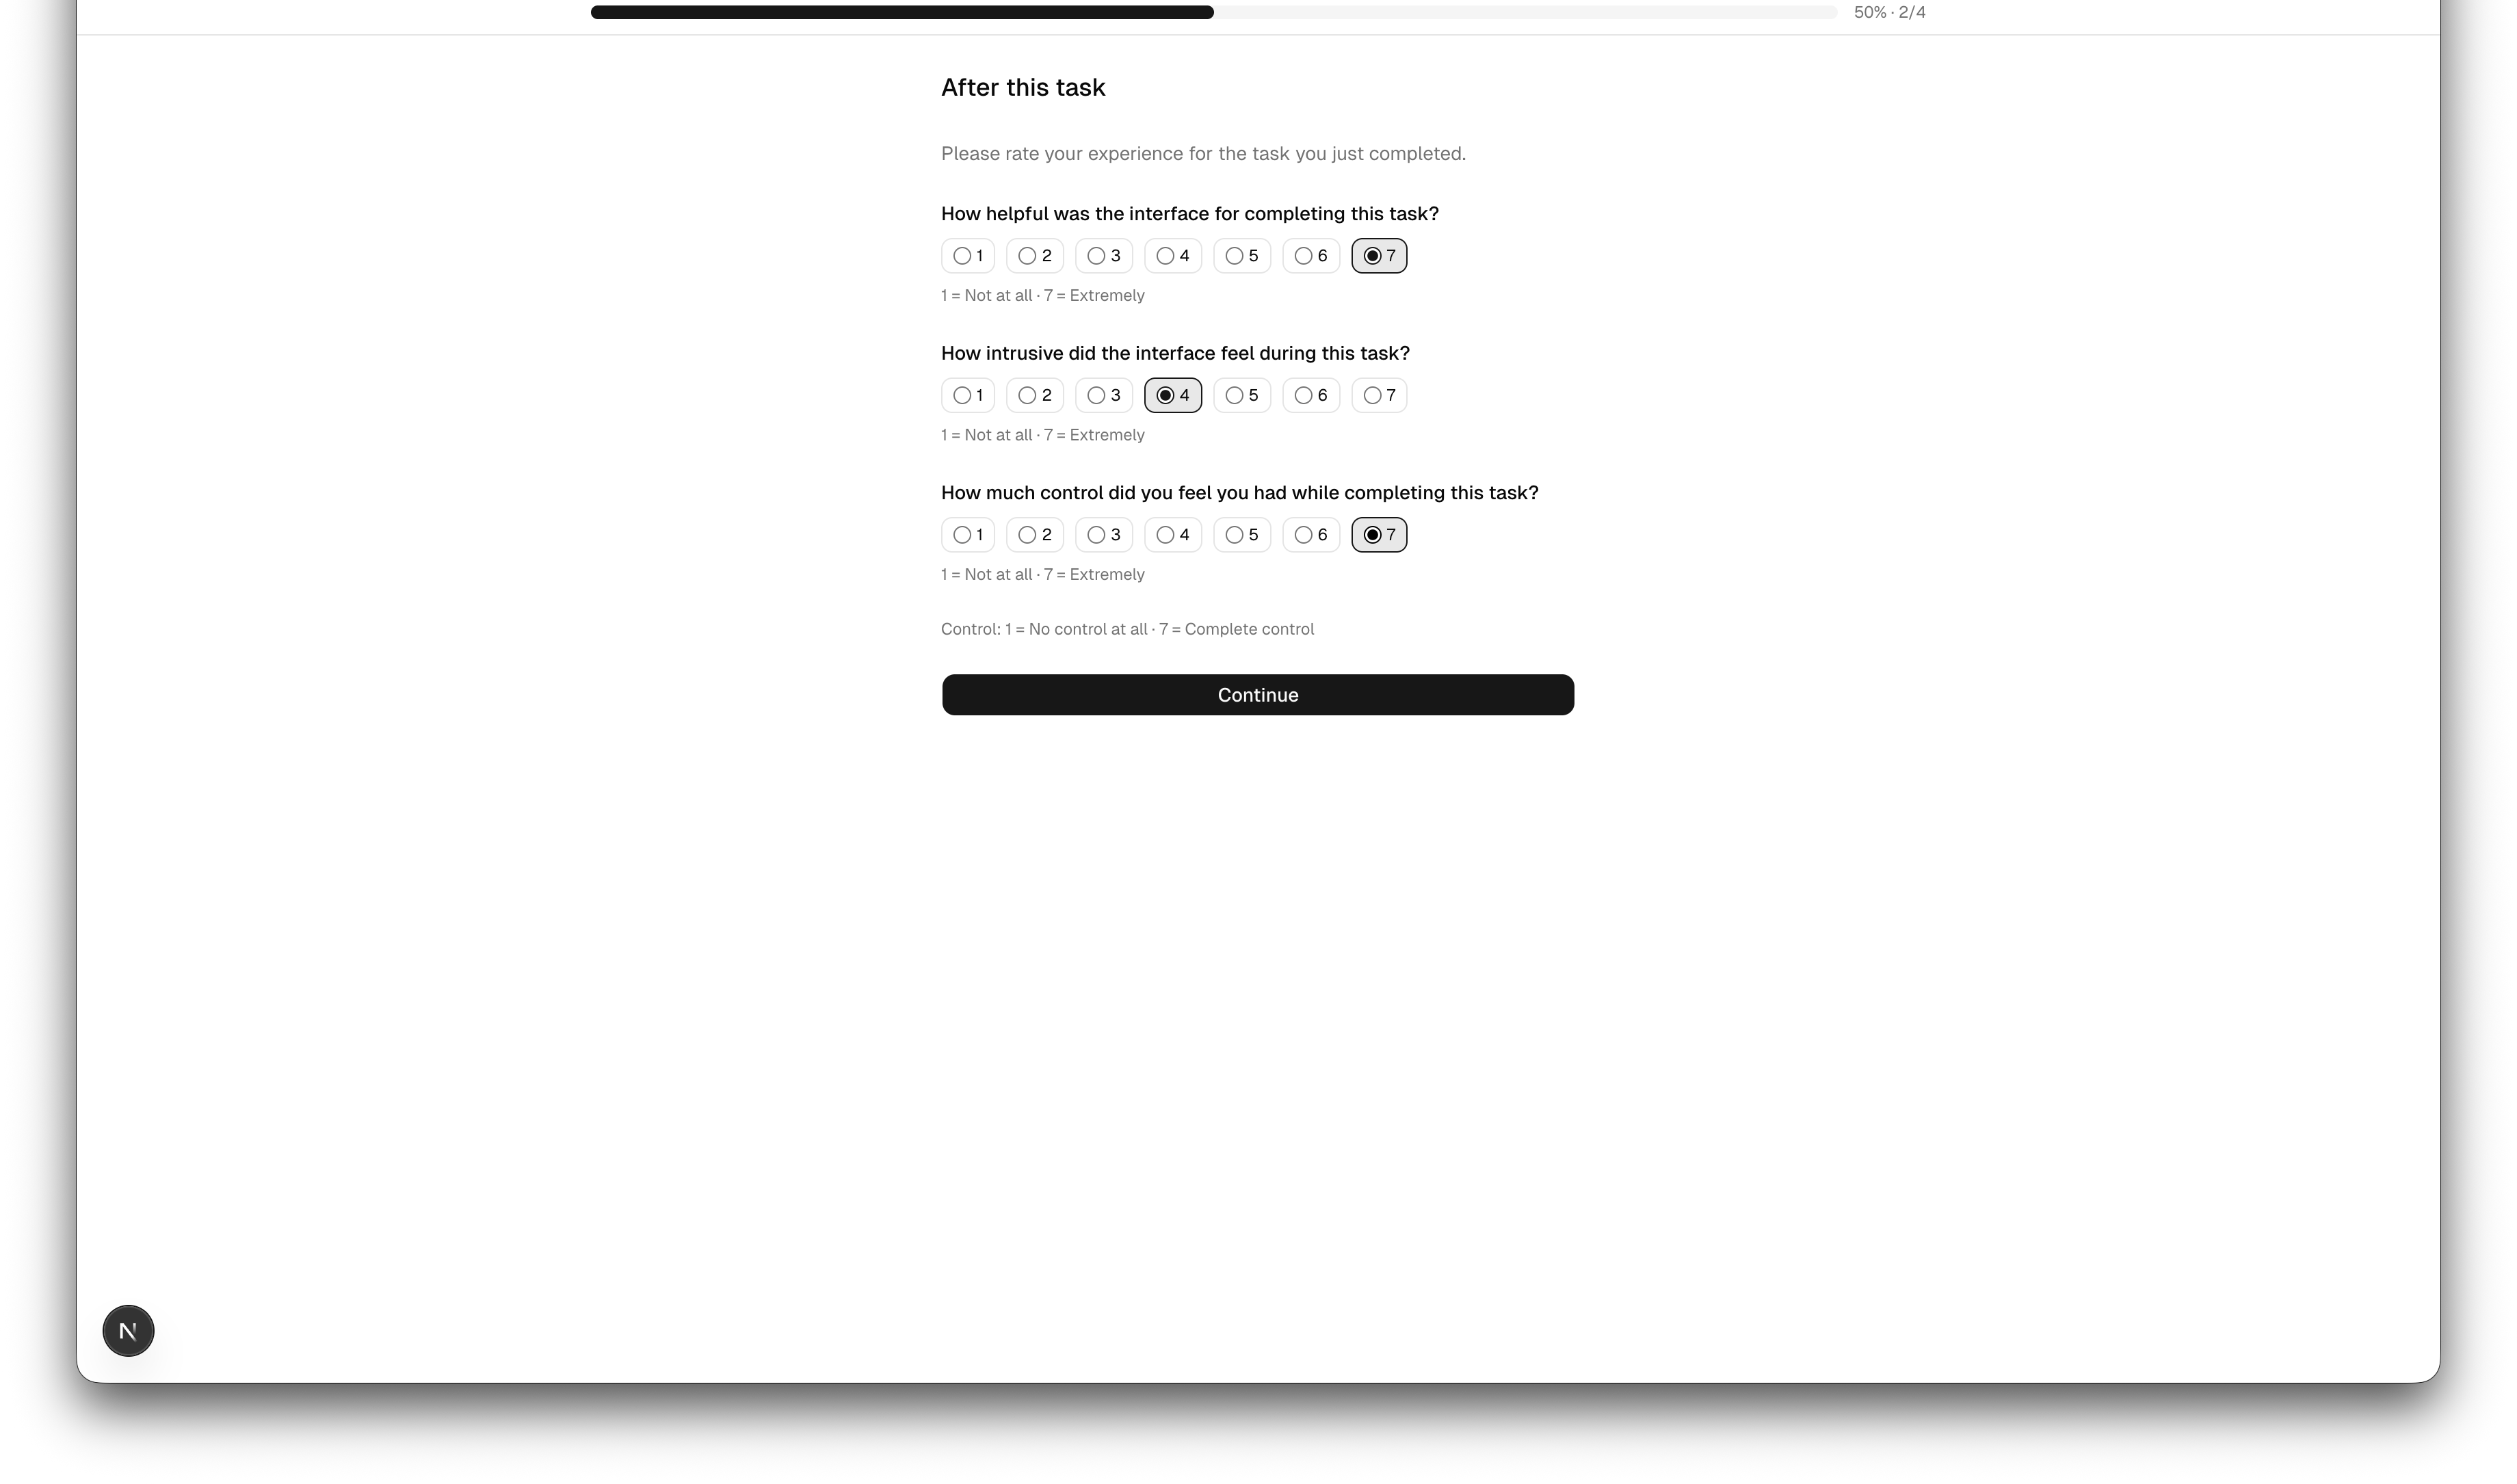
\includegraphics[width=\textwidth]{graphics/example-flow-3.png}
        \caption{Baseline post-trial questionnaire immediately after task completion.}
    \end{subfigure}
    \hfill
    \begin{subfigure}[t]{0.49\textwidth}
        \centering
        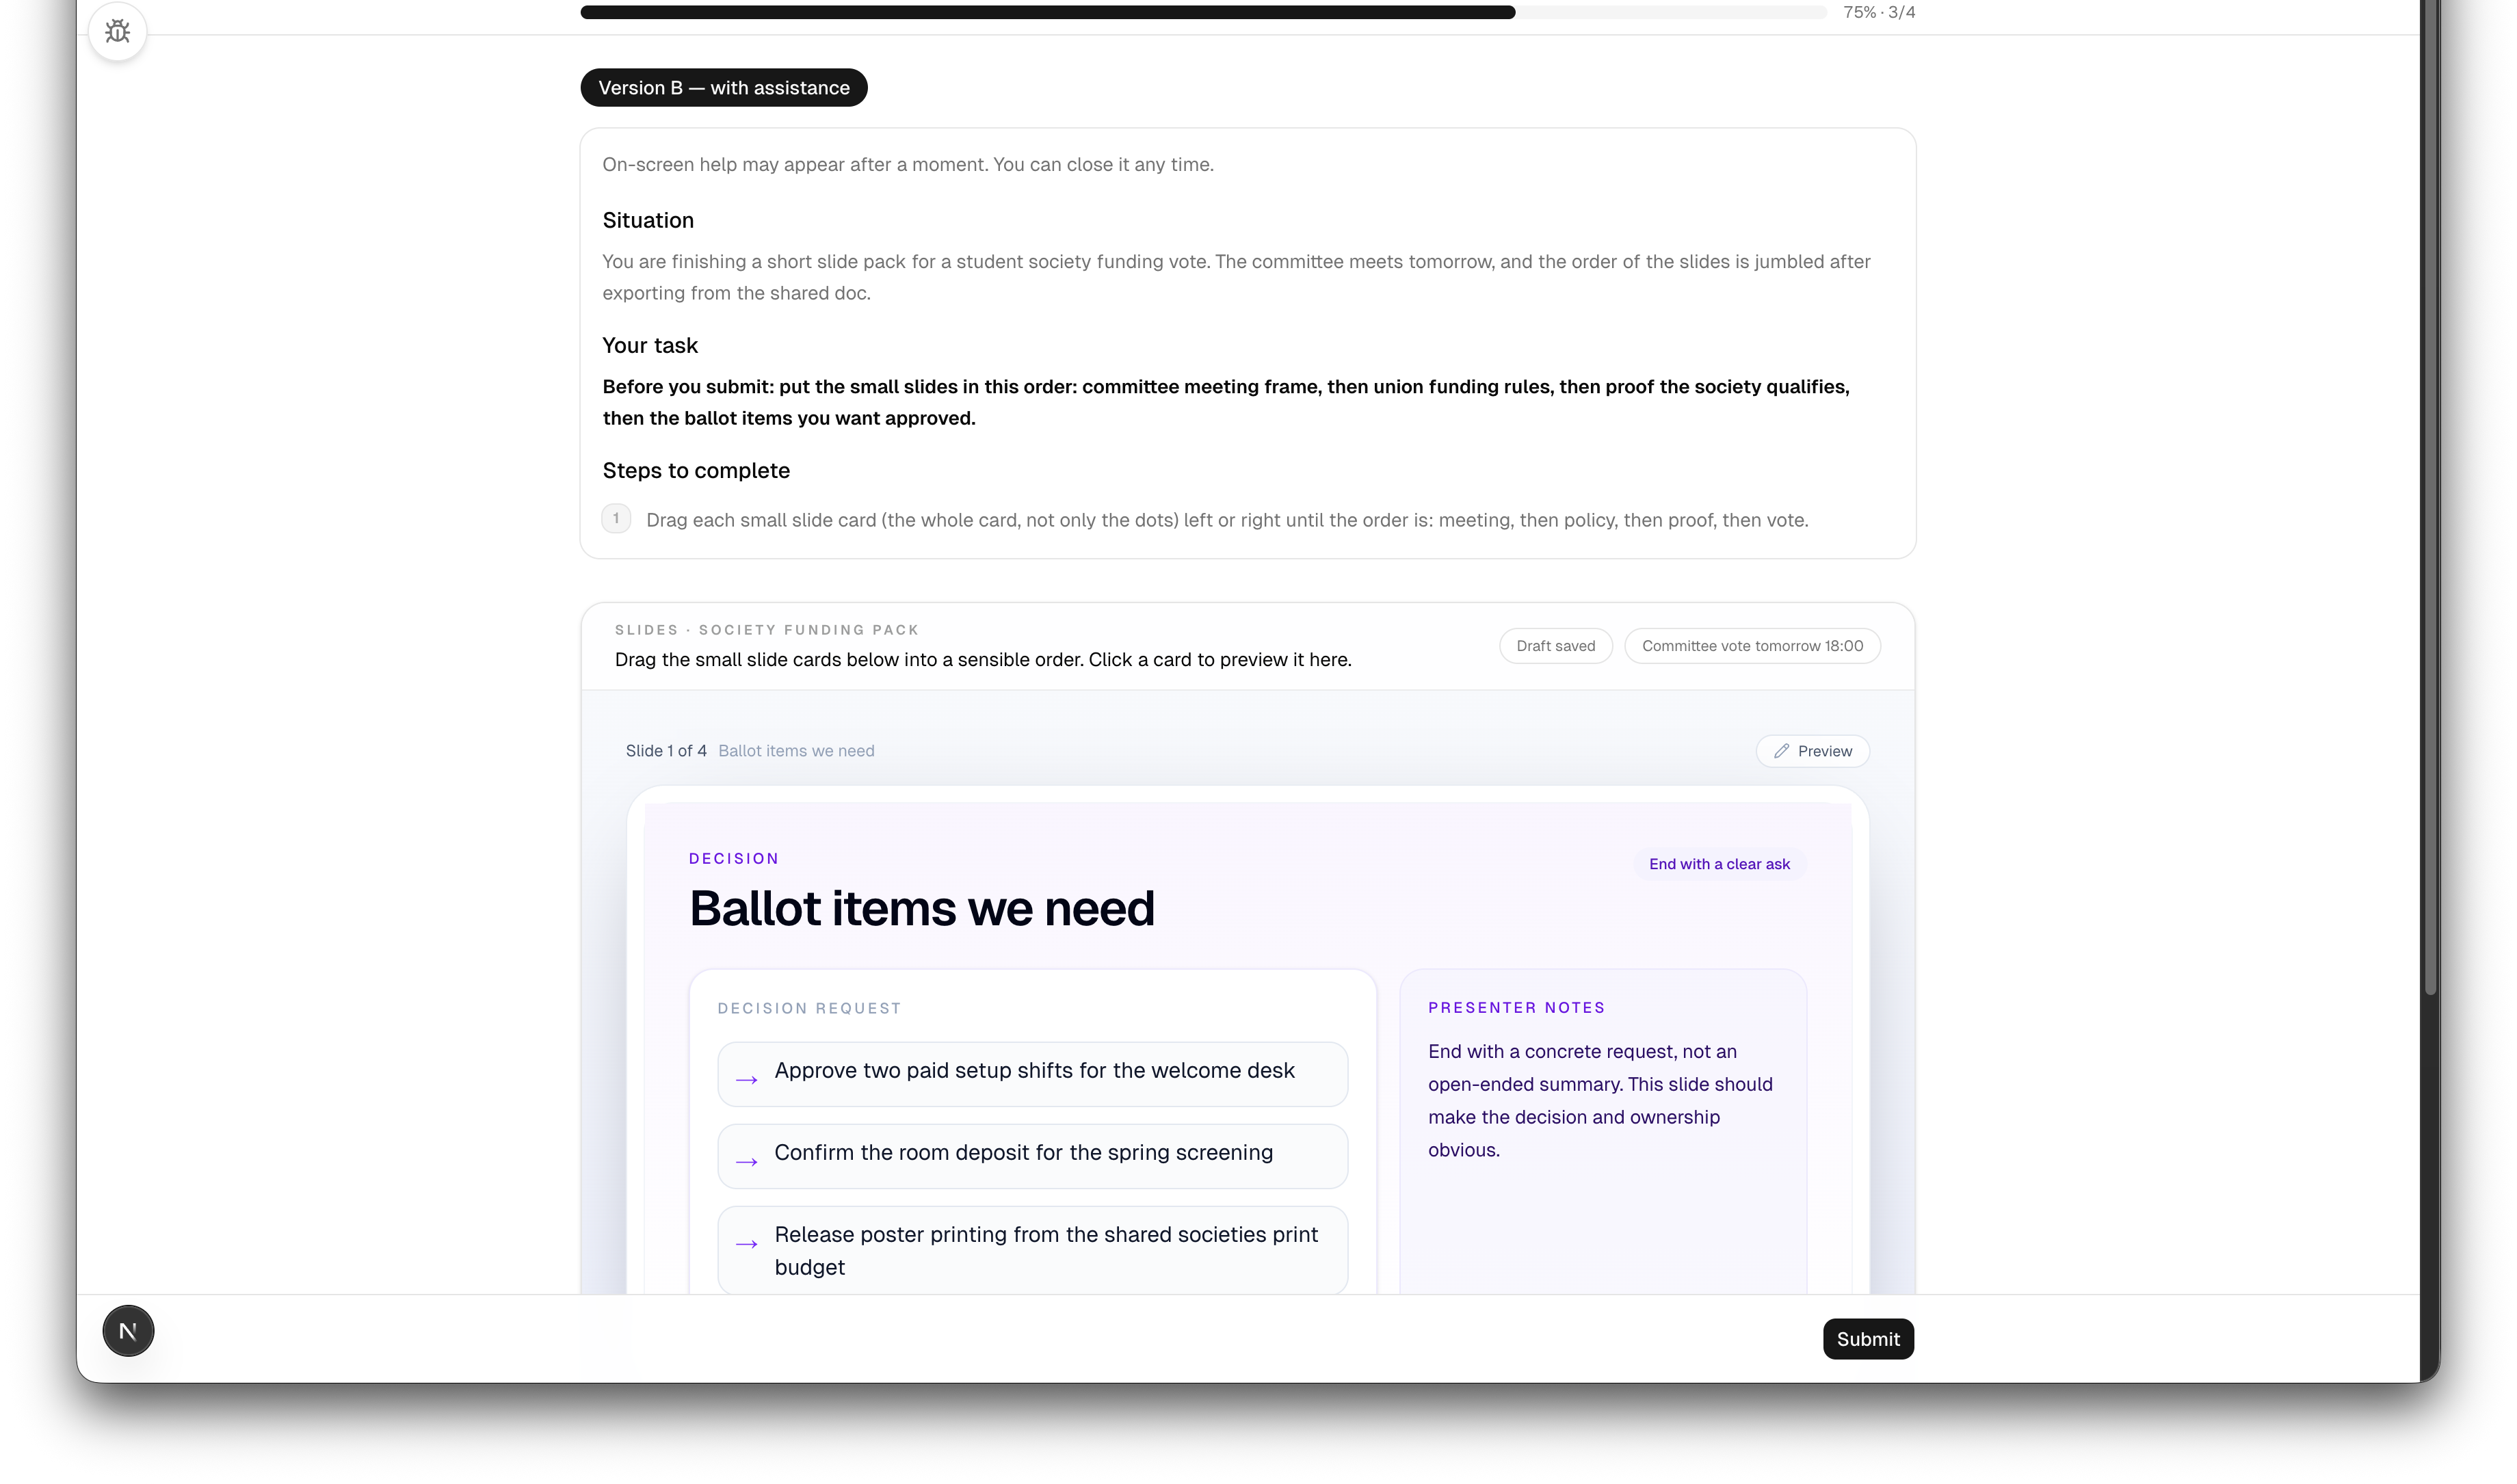
\includegraphics[width=\textwidth]{graphics/example-flow-4.png}
        \caption{Start of the ephemeral-condition trial, which warns that temporary help may appear.}
    \end{subfigure}
    \caption{Participant-flow walkthrough, part~2: transition from the baseline trial to the ephemeral trial.}
    \label{fig:appendix-flow-2}
\end{figure}

\begin{figure}[htbp]
    \centering
    \begin{subfigure}[t]{0.49\textwidth}
        \centering
        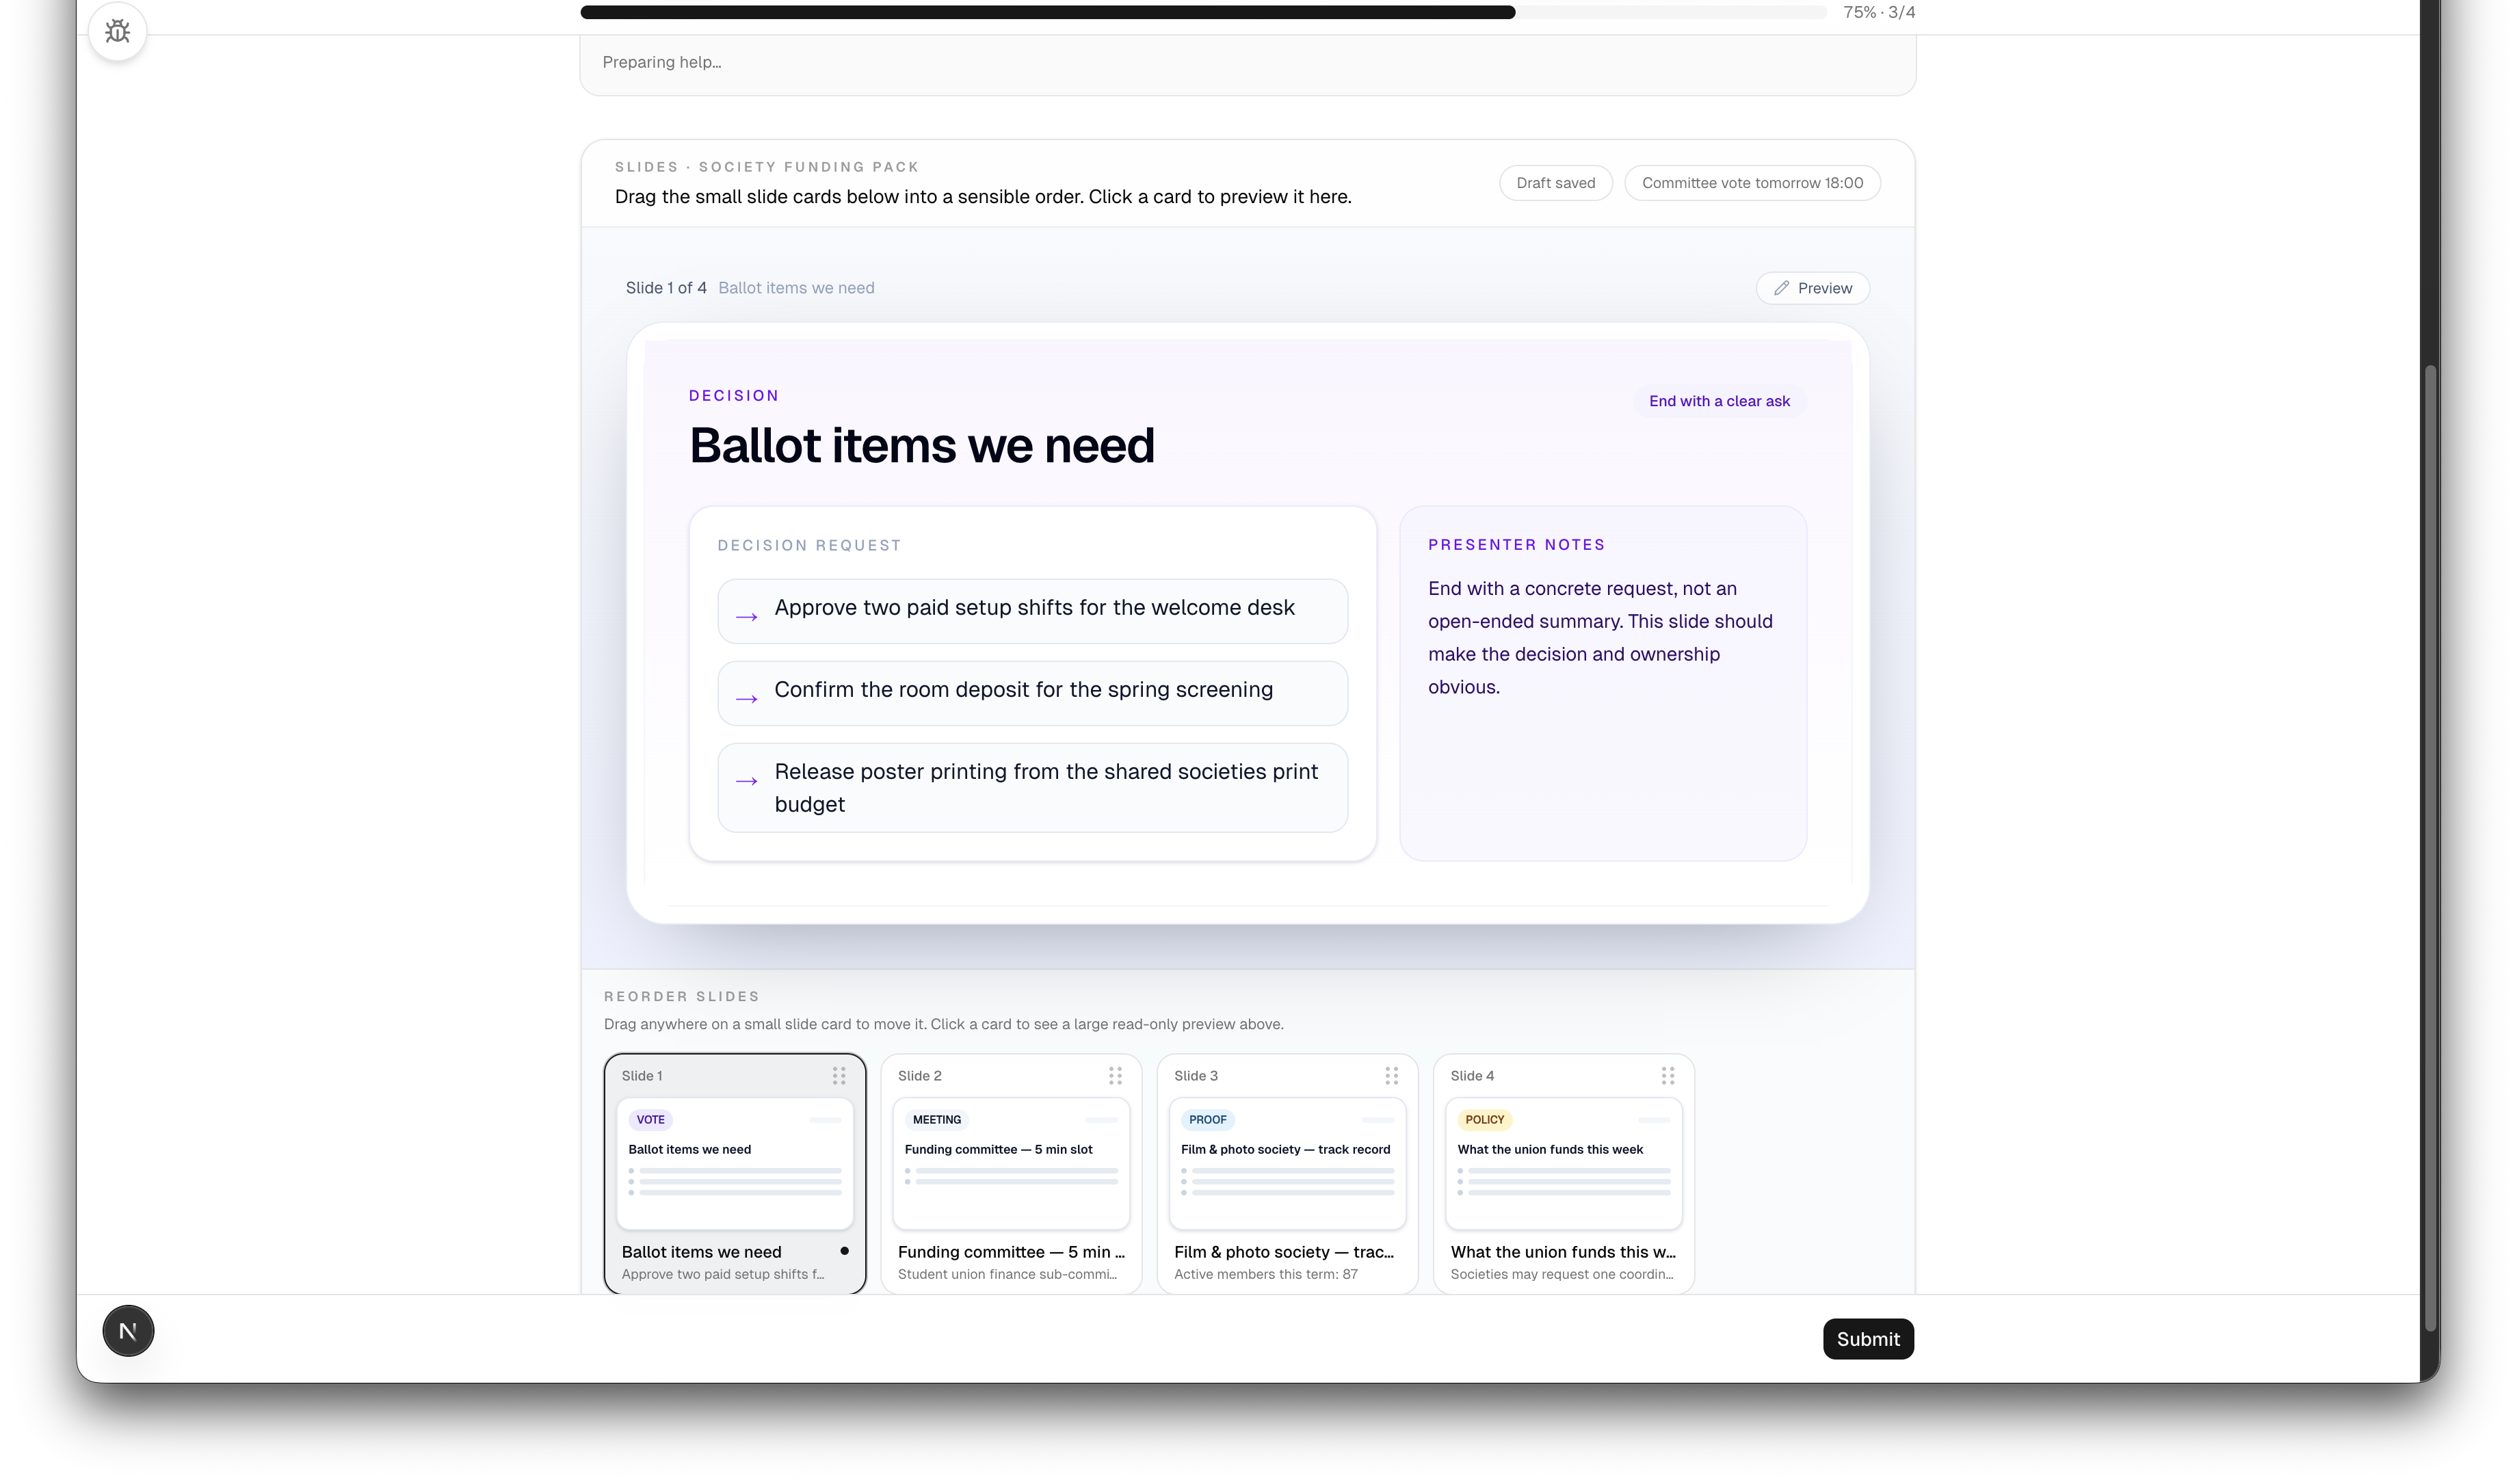
\includegraphics[width=\textwidth]{graphics/example-flow-5.png}
        \caption{Ephemeral-condition task before the support overlay expands.}
    \end{subfigure}
    \hfill
    \begin{subfigure}[t]{0.49\textwidth}
        \centering
        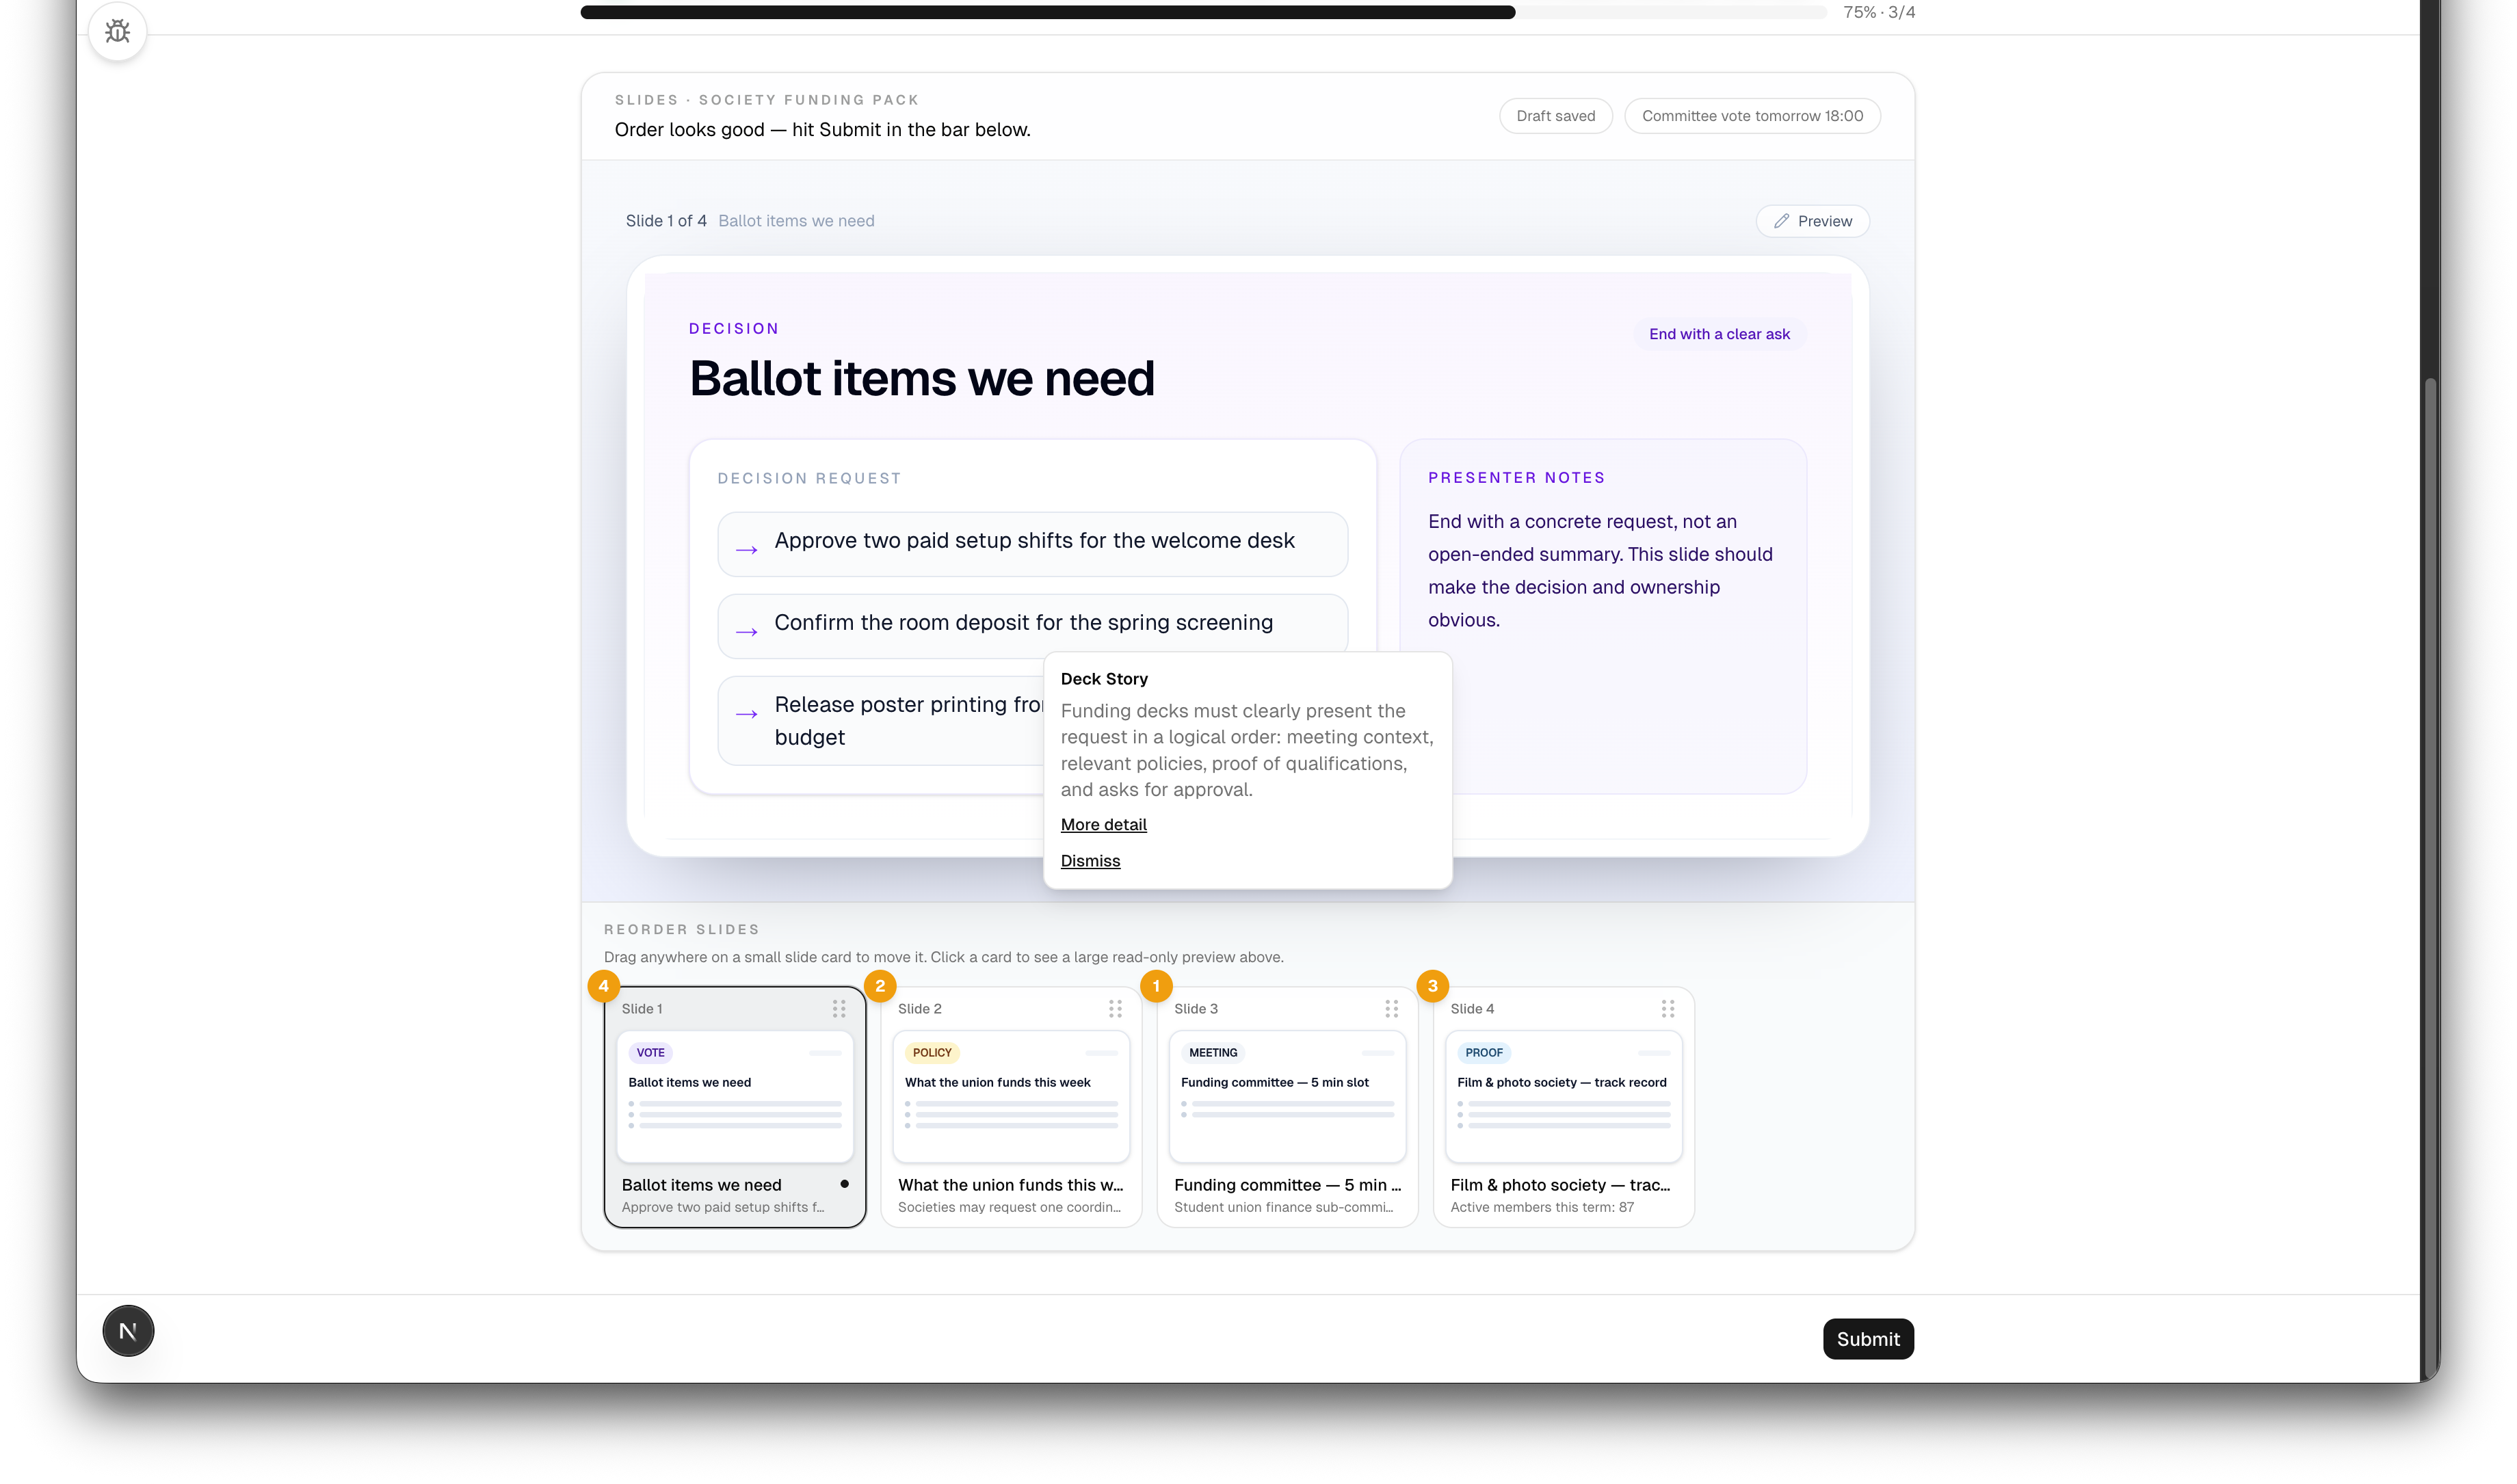
\includegraphics[width=\textwidth]{graphics/example-flow-6.png}
        \caption{Generated support visible as an anchored explanation and ordered markers over the slide strip.}
    \end{subfigure}
    \caption{Participant-flow walkthrough, part~3: ephemeral assistance becoming visible during the task.}
    \label{fig:appendix-flow-3}
\end{figure}

\begin{figure}[htbp]
    \centering
    \begin{subfigure}[t]{0.49\textwidth}
        \centering
        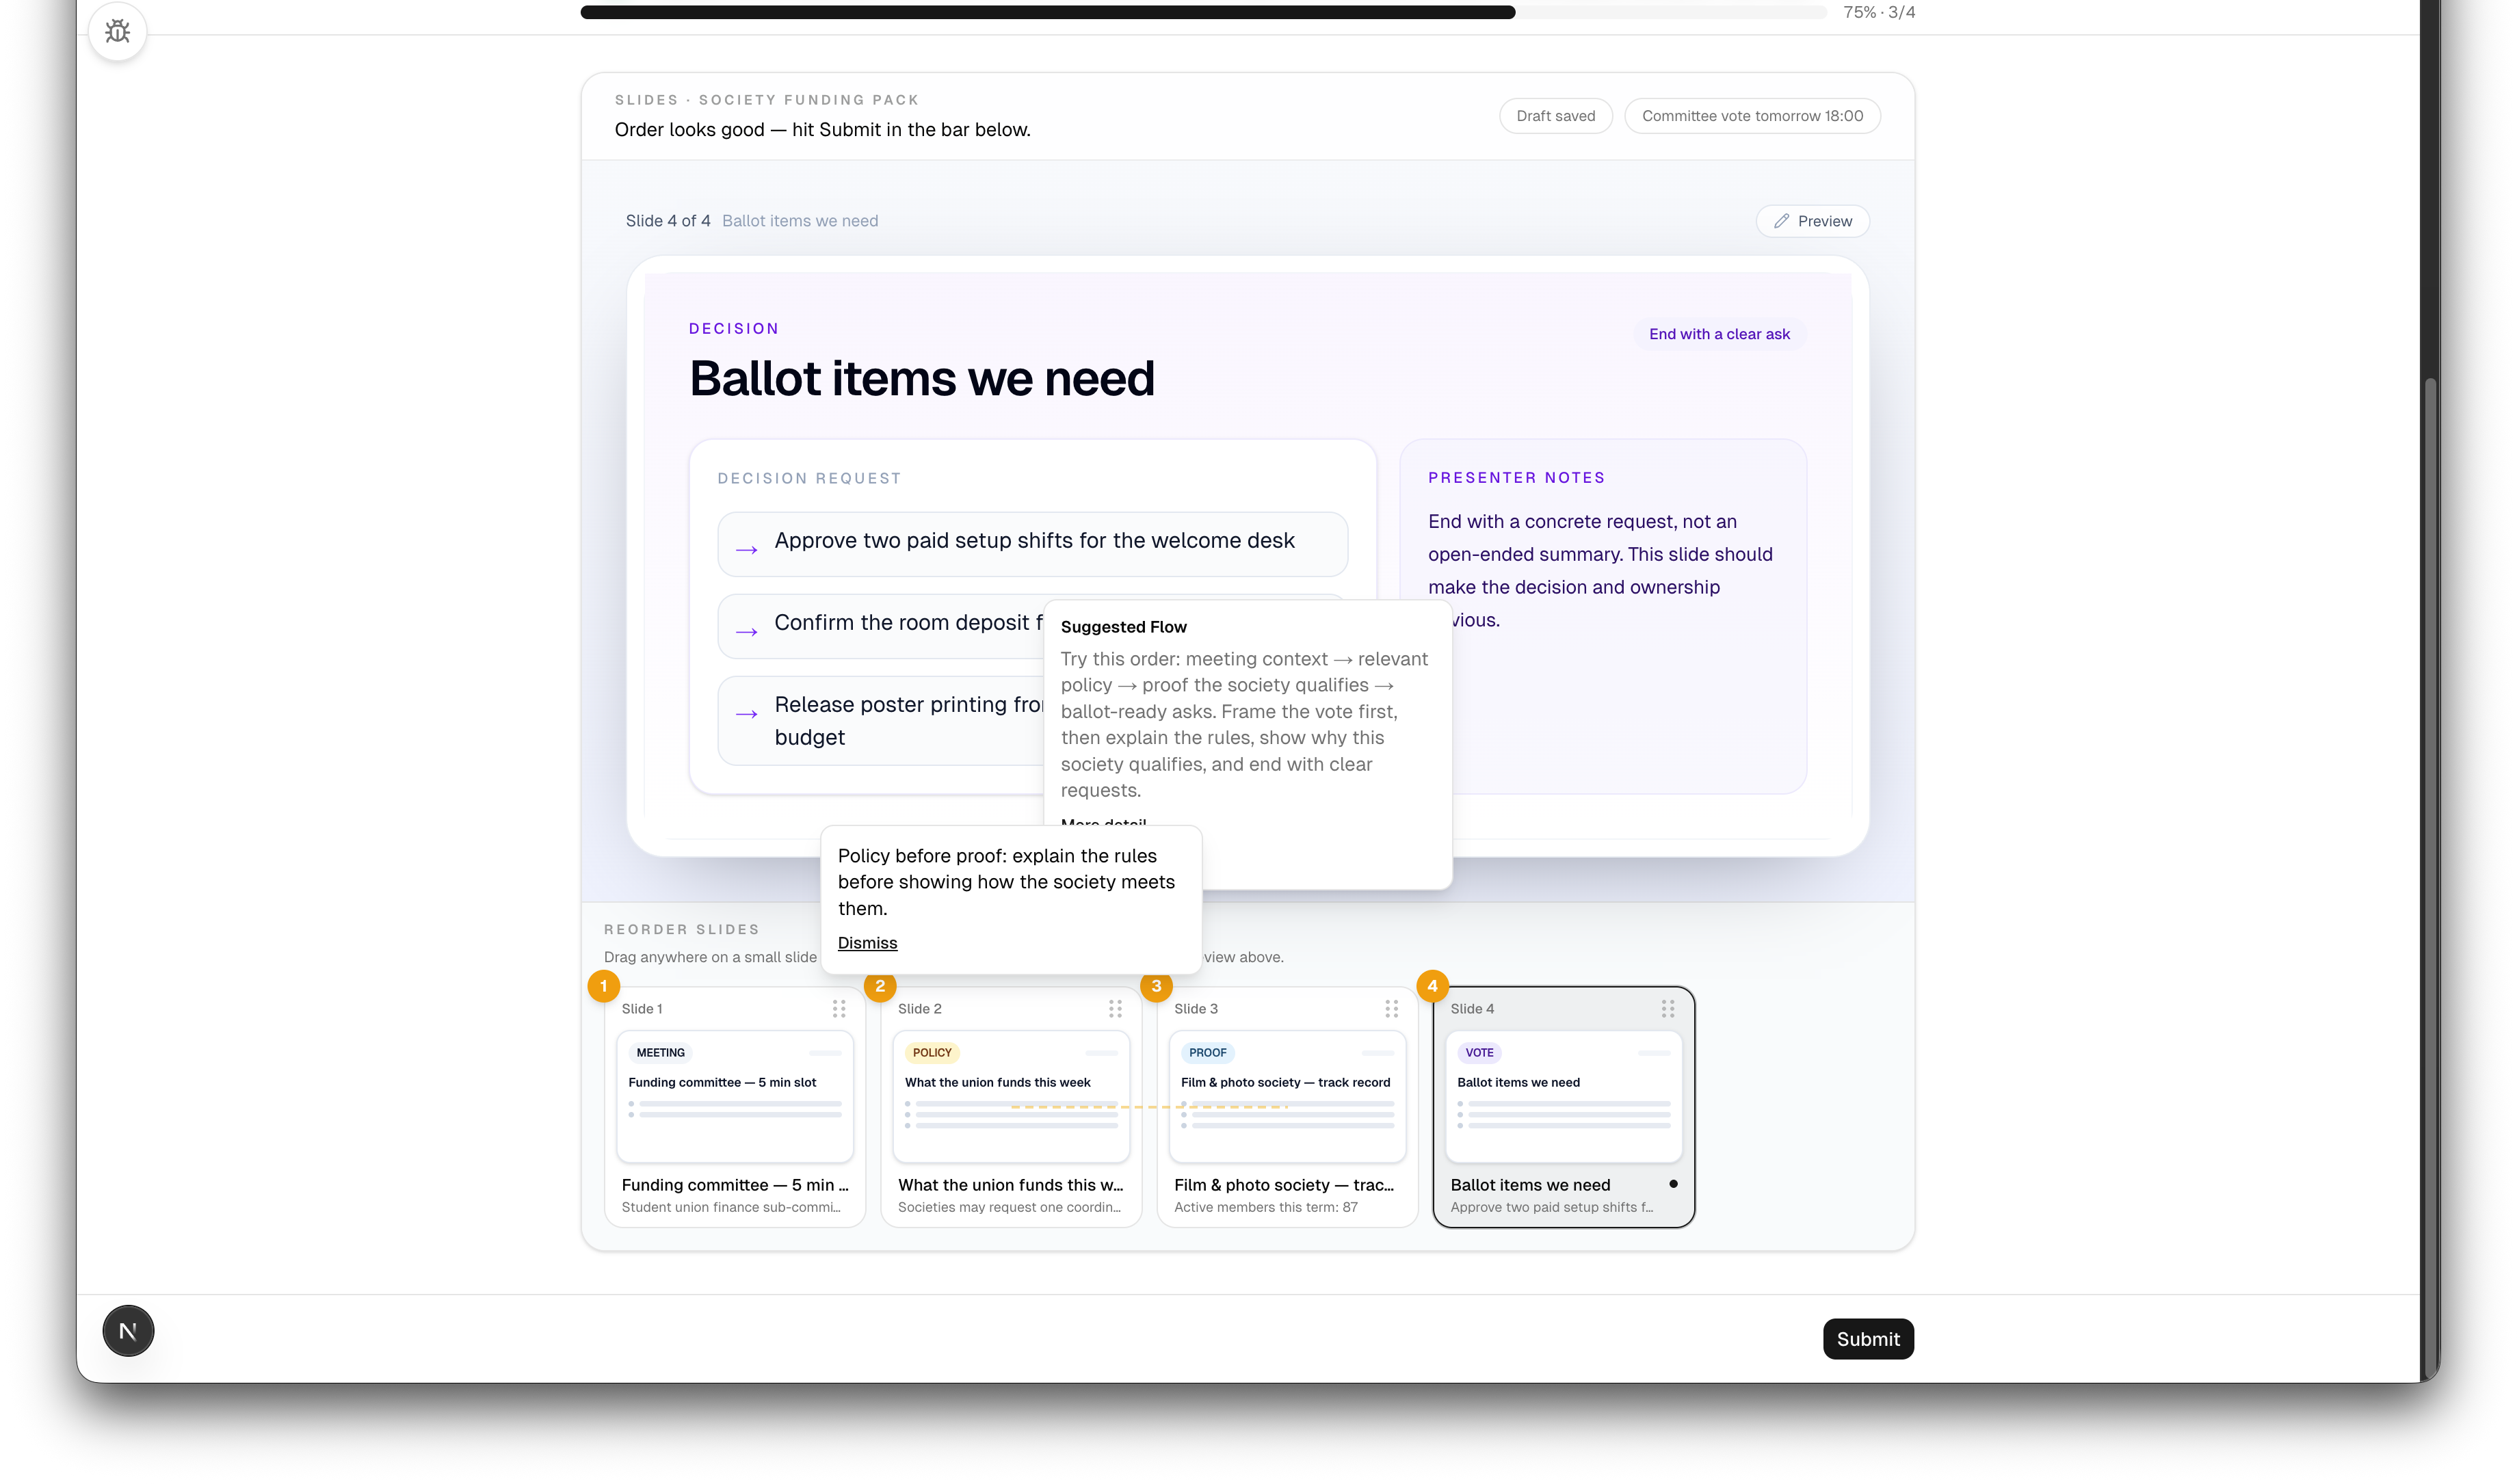
\includegraphics[width=\textwidth]{graphics/example-flow-7.png}
        \caption{Ephemeral overlay aligned to the current slide and reorder strip.}
    \end{subfigure}
    \hfill
    \begin{subfigure}[t]{0.49\textwidth}
        \centering
        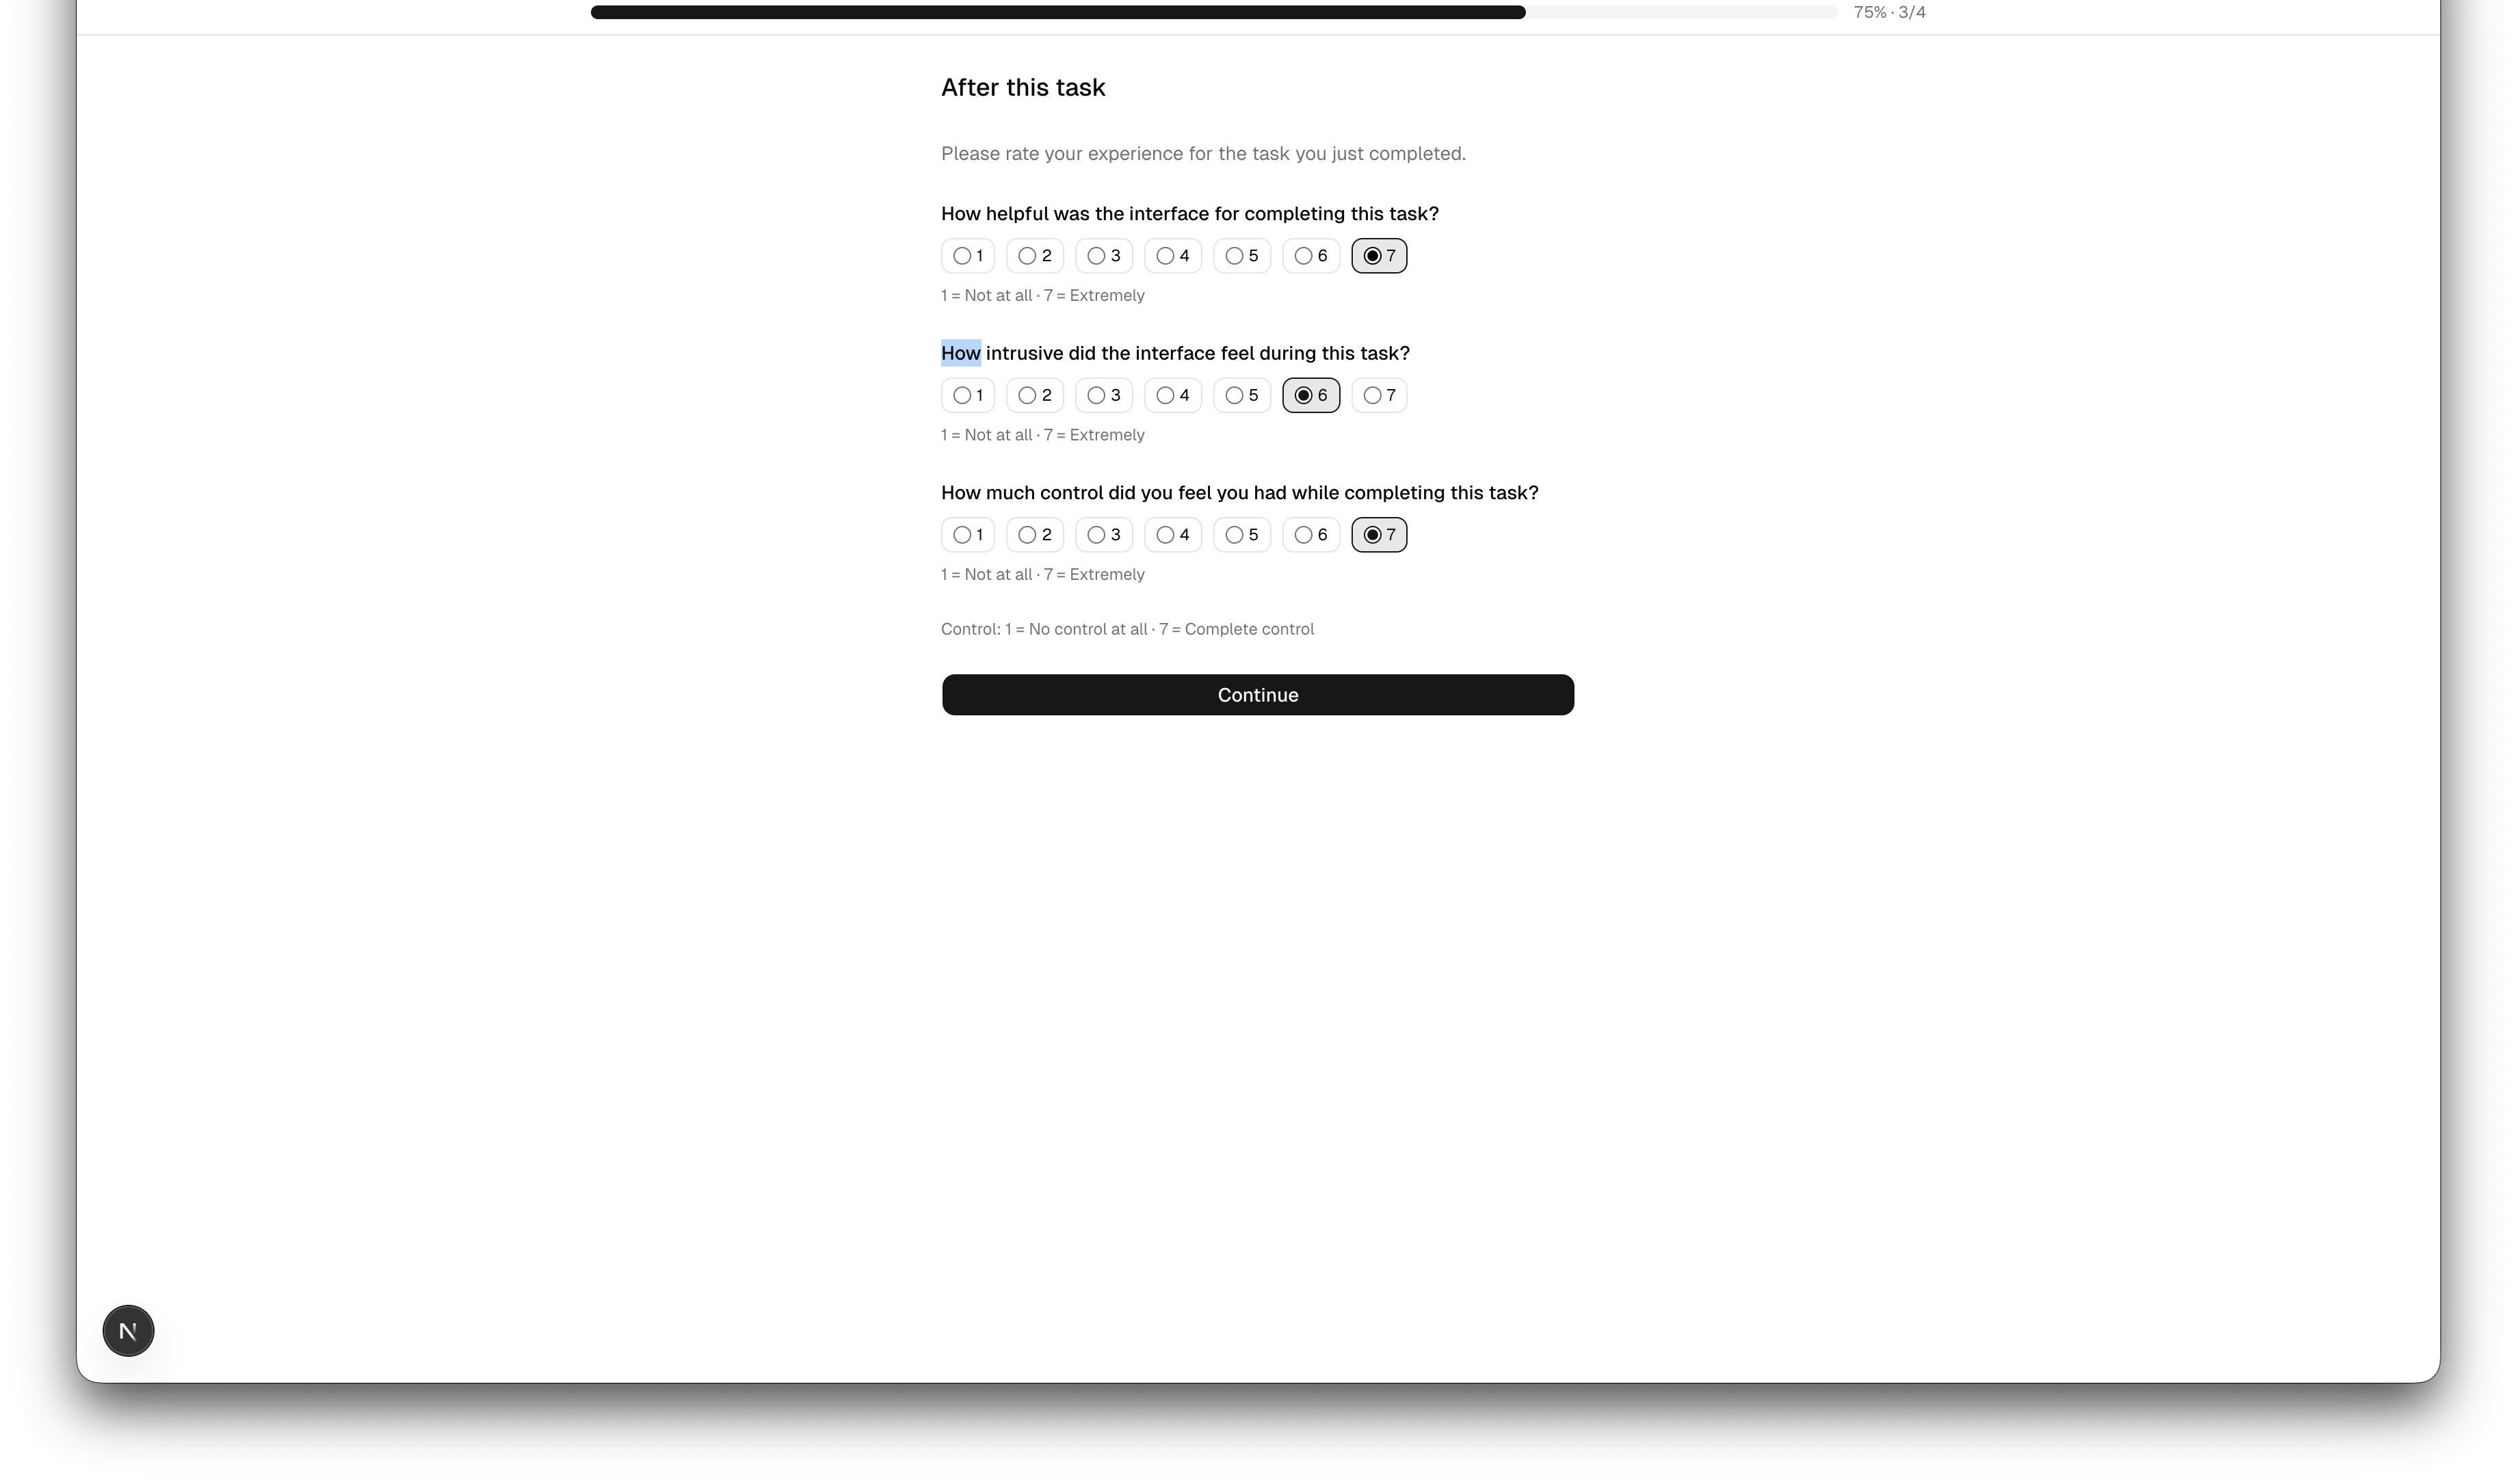
\includegraphics[width=\textwidth]{graphics/example-flow-8.png}
        \caption{Expanded support details combining an inspect panel, tooltip, and ordering cues.}
    \end{subfigure}
    \caption{Participant-flow walkthrough, part~4: richer support states within the ephemeral trial.}
    \label{fig:appendix-flow-4}
\end{figure}

\begin{figure}[htbp]
    \centering
    \begin{subfigure}[t]{0.49\textwidth}
        \centering
        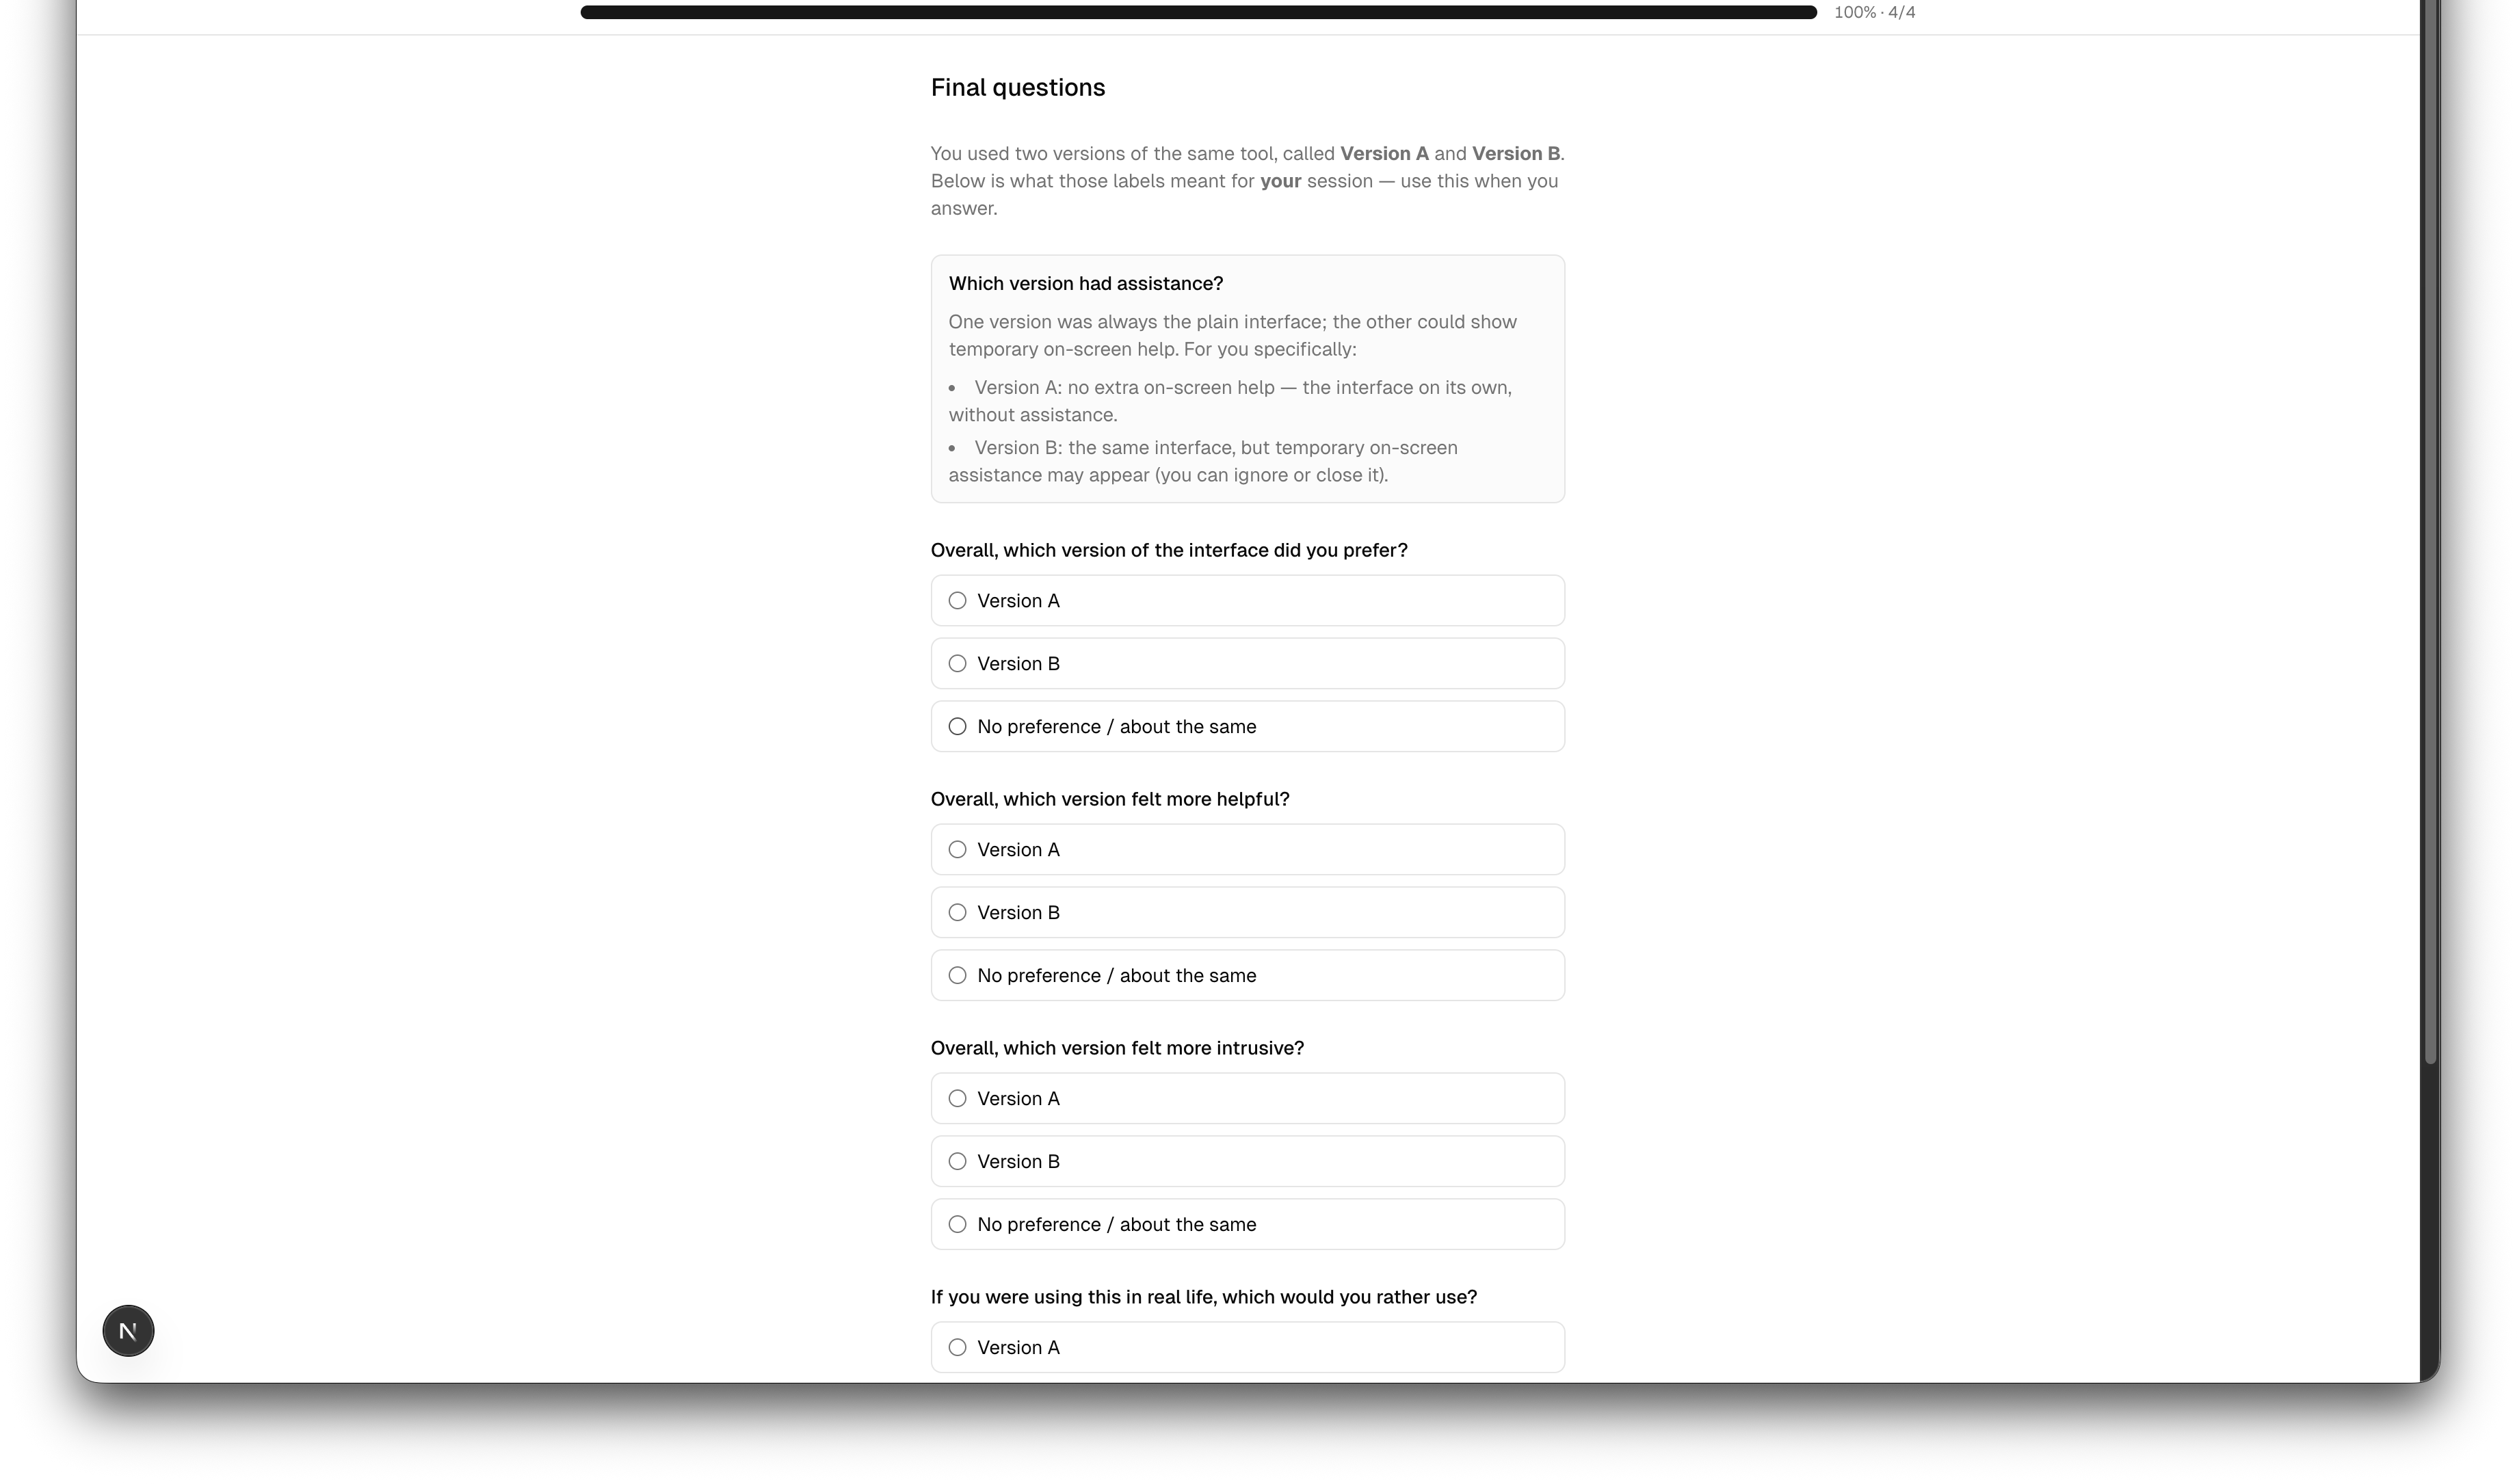
\includegraphics[width=\textwidth]{graphics/example-flow-9.png}
        \caption{Beginning of the final comparative questionnaire after both trials are complete.}
    \end{subfigure}
    \hfill
    \begin{subfigure}[t]{0.49\textwidth}
        \centering
        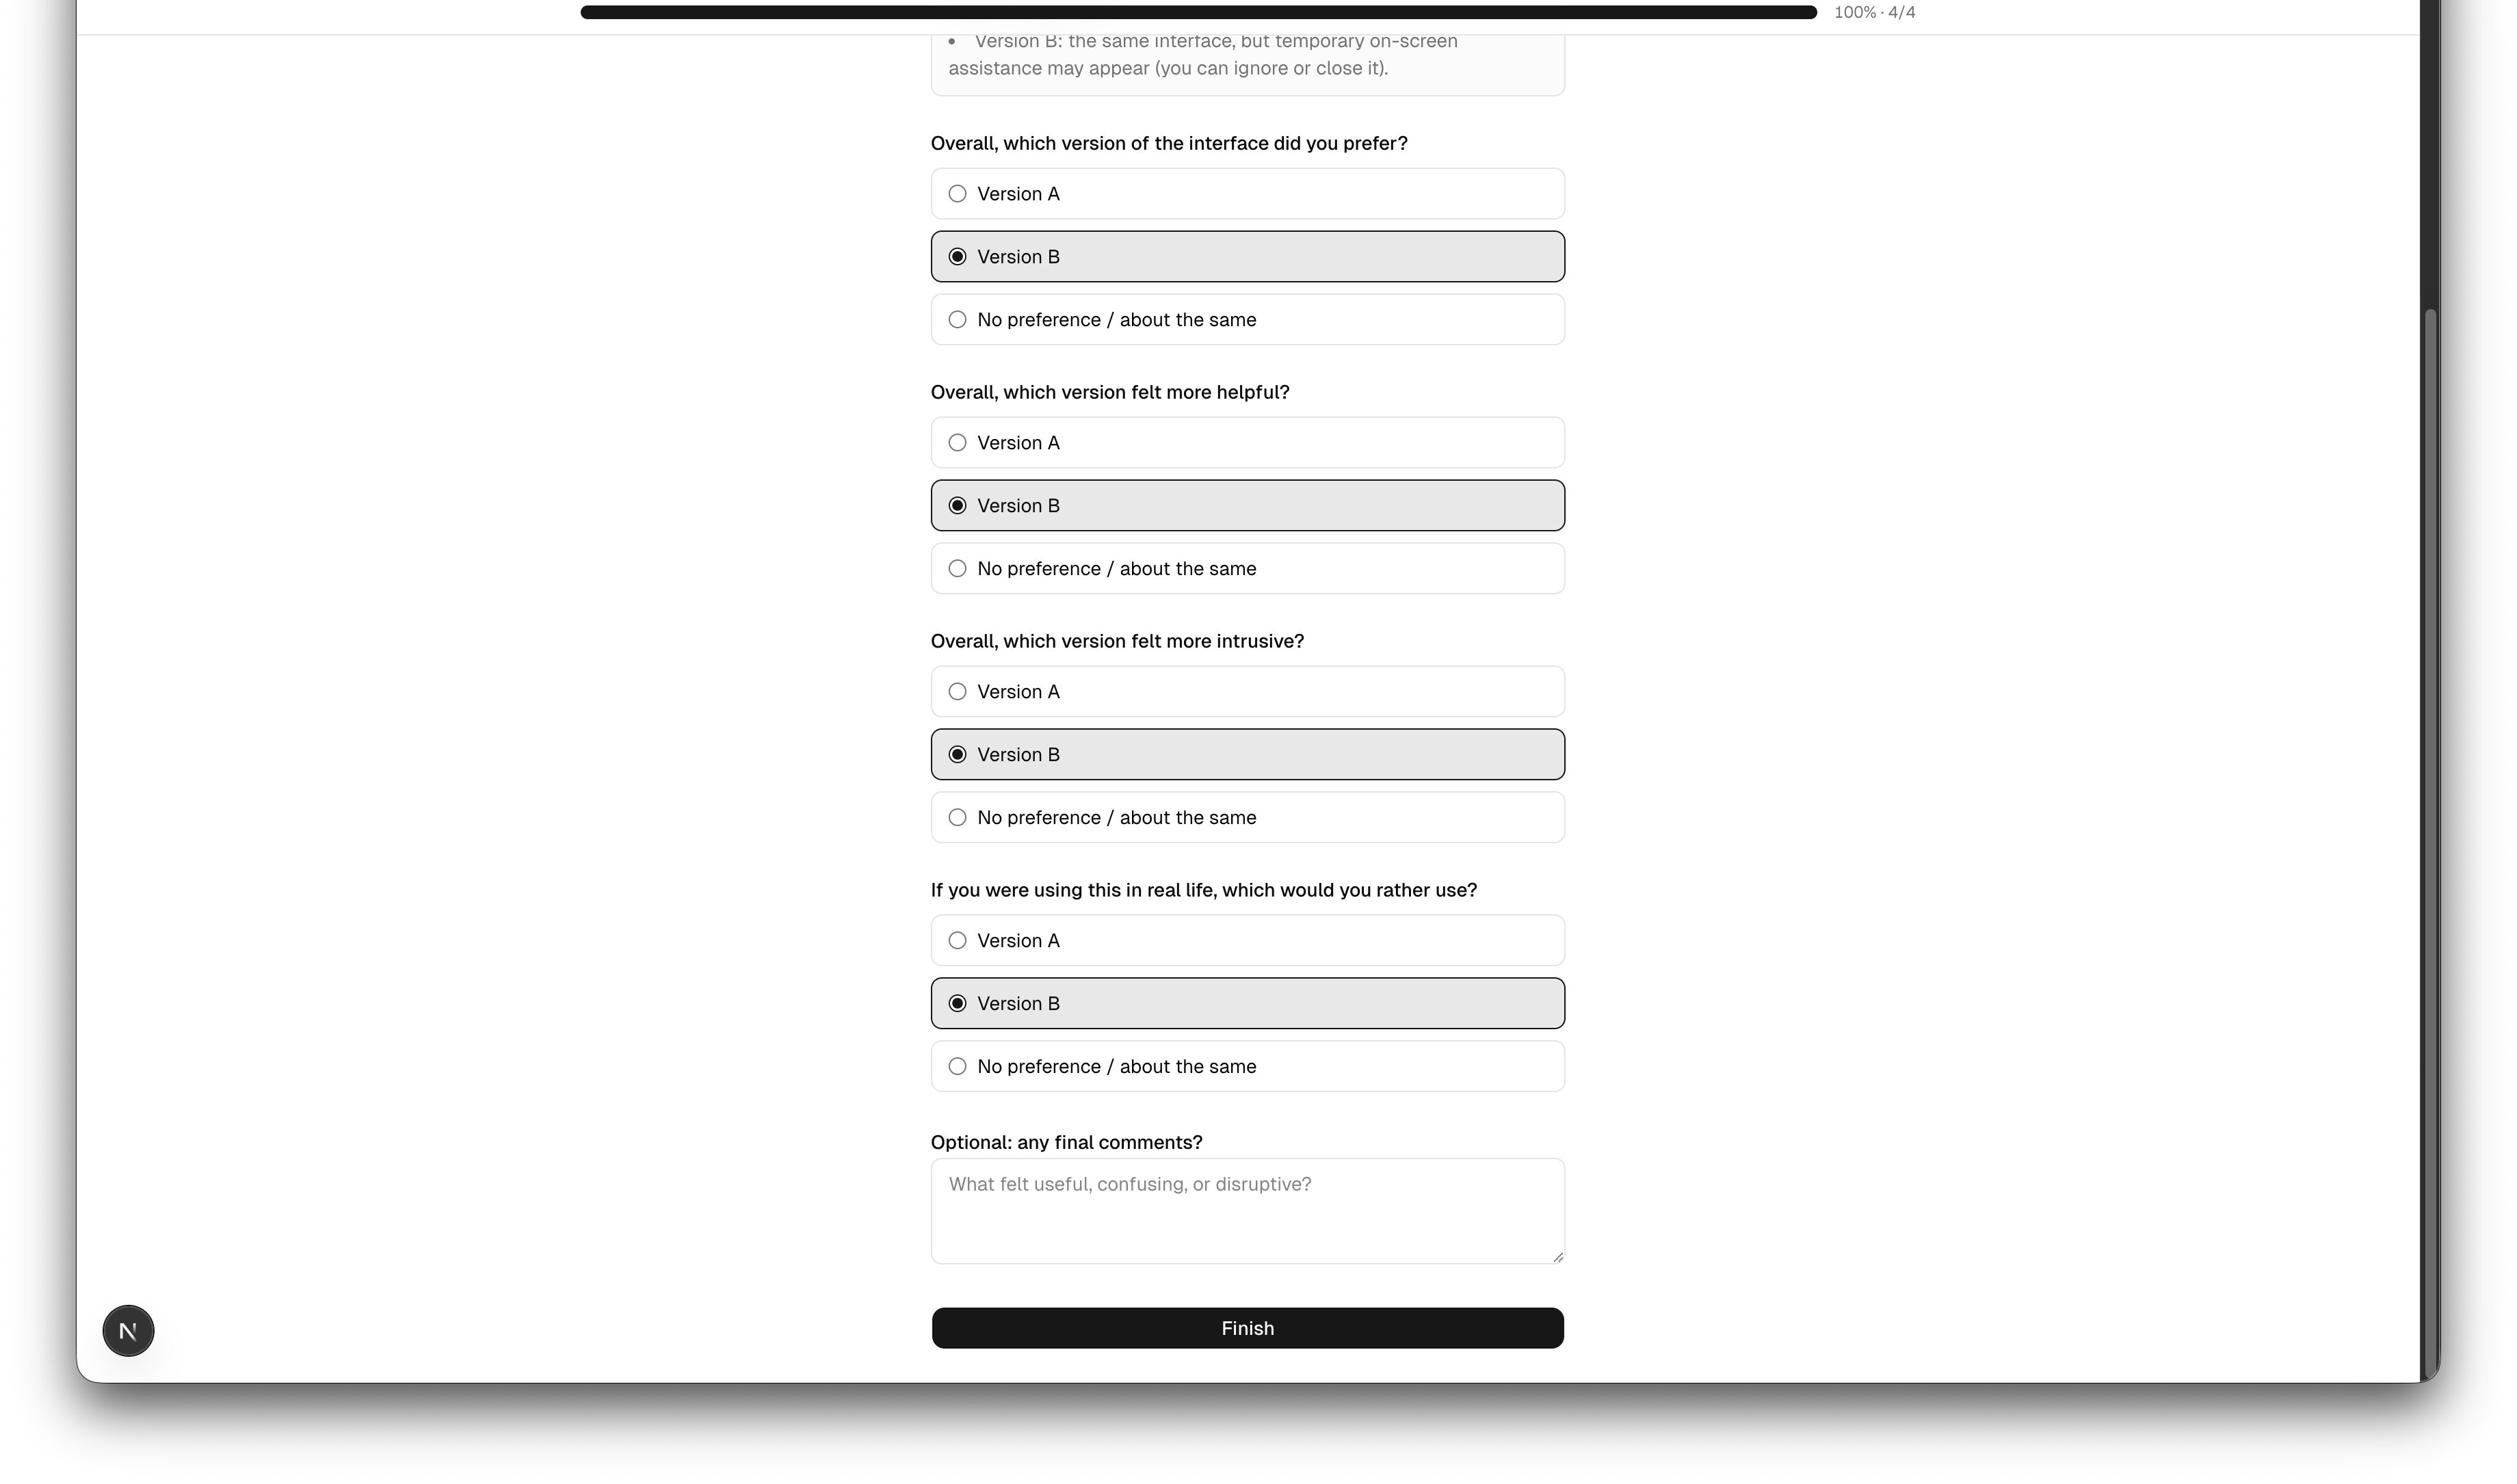
\includegraphics[width=\textwidth]{graphics/example-flow-11.png}
        \caption{Completed final questionnaire with comparative judgments recorded.}
    \end{subfigure}
    \caption{Participant-flow walkthrough, part~5: final comparison questions at the end of the session.}
    \label{fig:appendix-flow-5}
\end{figure}

\subsection{Interpretive Note}

These listings are sufficient to show the main route from raw study records to reported results: first the valid sample was defined consistently, then paired statistical tests were run, then publication-quality figures were generated, and finally the resulting numerical outputs were written into LaTeX commands consumed by the manuscript itself. This is the core evidence needed to demonstrate that the quantitative results chapter was generated through a reproducible analysis workflow rather than through manual transcription.

\end{appendices}


\printbibliography

\end{document}
